% Options for packages loaded elsewhere
\PassOptionsToPackage{unicode}{hyperref}
\PassOptionsToPackage{hyphens}{url}
\PassOptionsToPackage{dvipsnames,svgnames,x11names}{xcolor}
%
\documentclass[
]{krantz}
\usepackage{amsmath,amssymb}
\usepackage{iftex}
\ifPDFTeX
  \usepackage[T1]{fontenc}
  \usepackage[utf8]{inputenc}
  \usepackage{textcomp} % provide euro and other symbols
\else % if luatex or xetex
  \usepackage{unicode-math} % this also loads fontspec
  \defaultfontfeatures{Scale=MatchLowercase}
  \defaultfontfeatures[\rmfamily]{Ligatures=TeX,Scale=1}
\fi
\usepackage{lmodern}
\ifPDFTeX\else
  % xetex/luatex font selection
\fi
% Use upquote if available, for straight quotes in verbatim environments
\IfFileExists{upquote.sty}{\usepackage{upquote}}{}
\IfFileExists{microtype.sty}{% use microtype if available
  \usepackage[]{microtype}
  \UseMicrotypeSet[protrusion]{basicmath} % disable protrusion for tt fonts
}{}
\makeatletter
\@ifundefined{KOMAClassName}{% if non-KOMA class
  \IfFileExists{parskip.sty}{%
    \usepackage{parskip}
  }{% else
    \setlength{\parindent}{0pt}
    \setlength{\parskip}{6pt plus 2pt minus 1pt}}
}{% if KOMA class
  \KOMAoptions{parskip=half}}
\makeatother
\usepackage{xcolor}
\usepackage{longtable,booktabs,array}
\usepackage{calc} % for calculating minipage widths
% Correct order of tables after \paragraph or \subparagraph
\usepackage{etoolbox}
\makeatletter
\patchcmd\longtable{\par}{\if@noskipsec\mbox{}\fi\par}{}{}
\makeatother
% Allow footnotes in longtable head/foot
\IfFileExists{footnotehyper.sty}{\usepackage{footnotehyper}}{\usepackage{footnote}}
\makesavenoteenv{longtable}
\usepackage{graphicx}
\makeatletter
\def\maxwidth{\ifdim\Gin@nat@width>\linewidth\linewidth\else\Gin@nat@width\fi}
\def\maxheight{\ifdim\Gin@nat@height>\textheight\textheight\else\Gin@nat@height\fi}
\makeatother
% Scale images if necessary, so that they will not overflow the page
% margins by default, and it is still possible to overwrite the defaults
% using explicit options in \includegraphics[width, height, ...]{}
\setkeys{Gin}{width=\maxwidth,height=\maxheight,keepaspectratio}
% Set default figure placement to htbp
\makeatletter
\def\fps@figure{htbp}
\makeatother
\setlength{\emergencystretch}{3em} % prevent overfull lines
\providecommand{\tightlist}{%
  \setlength{\itemsep}{0pt}\setlength{\parskip}{0pt}}
\setcounter{secnumdepth}{5}
\usepackage{booktabs}
\usepackage{longtable}
\usepackage{hyperref}
\usepackage[bf,singlelinecheck=off]{caption}
\usepackage{geometry}
\geometry{margin=1in}

\usepackage{framed,color}
\definecolor{shadecolor}{RGB}{248,248,248}

\renewcommand{\textfraction}{0.05}
\renewcommand{\topfraction}{0.8}
\renewcommand{\bottomfraction}{0.8}
\renewcommand{\floatpagefraction}{0.75}

\renewenvironment{quote}{\begin{VF}}{\end{VF}}
\let\oldhref\href
\renewcommand{\href}[2]{#2\footnote{\url{#1}}}

\makeatletter
\newenvironment{kframe}{%
\medskip{}
\setlength{\fboxsep}{.8em}
 \def\at@end@of@kframe{}%
 \ifinner\ifhmode%
  \def\at@end@of@kframe{\end{minipage}}%
  \begin{minipage}{\columnwidth}%
 \fi\fi%
 \def\FrameCommand##1{\hskip\@totalleftmargin \hskip-\fboxsep
 \colorbox{shadecolor}{##1}\hskip-\fboxsep
     % There is no \\@totalrightmargin, so:
     \hskip-\linewidth \hskip-\@totalleftmargin \hskip\columnwidth}%
 \MakeFramed {\advance\hsize-\width
   \@totalleftmargin\z@ \linewidth\hsize
   \@setminipage}}%
 {\par\unskip\endMakeFramed%
 \at@end@of@kframe}
\makeatother

\usepackage{makeidx}
\makeindex

\urlstyle{tt}

\usepackage{amsthm}
\makeatletter
\def\thm@space@setup{%
  \thm@preskip=8pt plus 2pt minus 4pt
  \thm@postskip=\thm@preskip
}
\makeatother

\frontmatter
\usepackage{booktabs}
\usepackage{longtable}
\usepackage{array}
\usepackage{multirow}
\usepackage{wrapfig}
\usepackage{float}
\usepackage{colortbl}
\usepackage{pdflscape}
\usepackage{tabu}
\usepackage{threeparttable}
\usepackage{threeparttablex}
\usepackage[normalem]{ulem}
\usepackage{makecell}
\usepackage{xcolor}
\ifLuaTeX
  \usepackage{selnolig}  % disable illegal ligatures
\fi
\usepackage[]{natbib}
\bibliographystyle{apalike}
\usepackage{bookmark}
\IfFileExists{xurl.sty}{\usepackage{xurl}}{} % add URL line breaks if available
\urlstyle{same}
\hypersetup{
  pdftitle={Climate And Statistics},
  pdfauthor={Helmut Küchenhoff, Henri Funk},
  colorlinks=true,
  linkcolor={Maroon},
  filecolor={Maroon},
  citecolor={Blue},
  urlcolor={Blue},
  pdfcreator={LaTeX via pandoc}}

\title{Climate And Statistics}
\author{Helmut Küchenhoff, Henri Funk}
\date{2024-07-18}

\begin{document}
\maketitle

% you may need to leave a few empty pages before the dedication page

%\cleardoublepage\newpage\thispagestyle{empty}\null
%\cleardoublepage\newpage\thispagestyle{empty}\null
%\cleardoublepage\newpage
\thispagestyle{empty}

\begin{center}
\end{center}

\setlength{\abovedisplayskip}{-5pt}
\setlength{\abovedisplayshortskip}{-5pt}

{
\hypersetup{linkcolor=}
\setcounter{tocdepth}{0}
\tableofcontents
}
\chapter*{Preface}\label{preface}


\emph{Author: Henri Funk}

\begin{center}\includegraphics[width=0.75\linewidth]{cover} \end{center}

As the world faces the reality of climate change, natural hazards and extreme weather events have become a major concern, with devastating consequences for nature and humans. The quantification and definition of climate change, extreme events and its implications for life and health on our planet is one of the major concerns in climate science.

This book explains current statistical methods in climate science and their application.
The methods include compound events, low flow events and return periods, natural variability, teleconnections and causal discovery.
All of those methods are used to quantify and anticipate the changing climate.

This book is the outcome of the seminar ``Climate and Statistics'' which took place in summer 2024 at the Department of Statistics, LMU Munich.

\begin{figure}
\centering
\includegraphics{by-nc-sa.png}
\caption{Creative Commons License}
\end{figure}

This book is licensed under the \href{http://creativecommons.org/licenses/by-nc-sa/4.0/}{Creative Commons Attribution-NonCommercial-ShareAlike 4.0 International License}.

\mainmatter

\chapter*{Foreword}\label{foreword}


\emph{Author: Christoph Molnar}

This book is the result of an experiment in university teaching.
Each semester, students of the Statistics Master can choose from a selection of seminar topics.
Usually, every student in the seminar chooses a scientific paper, gives a talk about the paper and summarizes it in the form of a seminar paper.
The supervisors help the students, they listen to the talks, read the seminar papers, grade the work and then \ldots{} hide the seminar papers away in (digital) drawers.
This seemed wasteful to us, given the huge amount of effort the students usually invest in seminars.
An idea was born:
Why not create a book with a website as the outcome of the seminar?
Something that will last at least a few years after the end of the semester.
In the summer term 2019, some Statistics Master students signed up for our seminar entitled ``Limitations of Interpretable Machine Learning''.
When they came to the kick-off meeting, they had no idea that they would write a book by the end of the semester.

We were bound by the examination rules for conducting the seminar, but otherwise we could deviate from the traditional format.
We deviated in several ways:

\begin{enumerate}
\def\labelenumi{\arabic{enumi}.}
\tightlist
\item
  Each student project is part of a book, and not an isolated seminar paper.
\item
  We gave challenges to the students, instead of papers. The challenge was to investigate a specific limitation of interpretable machine learning methods.
\item
  We designed the work to live beyond the seminar.
\item
  We emphasized collaboration. Students wrote some chapters in teams and reviewed each others texts.
\end{enumerate}

\section*{Technical Setup}\label{technical-setup}


The book chapters are written in the Markdown language.
The simulations, data examples and visualizations were created with R \citep{rlang}.
To combine R-code and Markdown, we used rmarkdown.
The book was compiled with the bookdown package.
We collaborated using git and github.
For details, head over to the \href{https://github.com/henrifnk/Seminar_ClimateNStatistics}{book's repository}.

\chapter{Introduction}\label{introduction}

\emph{Author: }

\emph{Supervisor: }

\section{Intro About the Seminar Topic}\label{intro-about-the-seminar-topic}

\section{Outline of the Booklet}\label{outline-of-the-booklet}

\chapter{Natural Variability by internal variability}\label{iv}

\emph{Author: Senta Roßmayer}

\emph{Supervisor: Henri Funk}

\emph{Suggested degree: Bachelor}

\section{Abstract}\label{abstract}

Natural variability refers to the inherent fluctuations in the climate system that occur without external forcings, such as changes in solar radiation, volcanic eruptions, or human-induced alterations of the Earth's atmosphere and surface. This variability can be due to a variety of factors, including atmospheric processes, ocean currents, the El Niño-Southern Oscillation (ENSO), and other dynamic components of the Earth system. Natural variability occurs across all time scales, from short-term (daily, seasonal) to long-term (decadal, centennial) fluctuations.

\section{Climate Model Ensemble}\label{climate-model-ensemble}

Climate models are sophisticated tools that simulate the interactions within the Earth's climate system. To understand and quantify natural variability, scientists use ensembles of climate model simulations. An ensemble consists of multiple runs of the same model, or different models, where each run has slightly different initial conditions or model parameters. This approach helps to capture the range of possible climate outcomes due to the inherent uncertainty and variability in the system.

\section{Internal Variability}\label{internal-variability}

Within the context of climate model ensembles, internal variability refers to the variations in climate that arise from the system's internal processes, independent of external forcings. This variability is a fundamental part of the climate system's dynamics and can lead to different outcomes even if the external conditions are the same.

\section{1. Introduction to climate modelling and climate variability}\label{introduction-to-climate-modelling-and-climate-variability}

The Earth's climate is a complex system that is characterised by diverse and interrelated physical, chemical and biological processes. Climate models play a central role in analysing and predicting this system. They enable scientists to simulate and analyse the reactions of the Earth's atmosphere, oceans and land surfaces to various influences. By using them, past climate changes can be reconstructed and future climate trends and extremes can be predicted.
The fundamentals of climate modelling include understanding the basic physical principles that regulate the exchange and distribution of energy and mass within the climate system. These models are based on mathematical representations of physical processes and use complex algorithms to calculate these representations. These calculations are performed repeatedly to simulate the dynamic changes of the climate system over time (\citet{eyring2016overview}). A sound knowledge of the physical processes, such as radiative transfer, turbulent fluxes and the dynamics of the atmosphere and oceans, is essential for the development and interpretation of these models (\citet{latif2022natural}).
Another important aspect of climate modelling is the consideration of climate variability. Climate variability refers to natural fluctuations in the climate system that can occur on different time scales, from a few years to centuries or even millennia. This variability can have various causes, including internal processes such as the North Atlantic Oscillation or global phenomena such as El Niño (\citet{deser}). It is crucial to distinguish between short-term climatic fluctuations and long-term trends in order to make more accurate climate projections.
Various types of climate models are used in research, which differ in their complexity and scope of application. These range from simple energy-equilibrium models that consider basic climate variables to highly complex coupled atmosphere-ocean models that consider a variety of climate components and interactions (\citet{eyring2016overview}). The Coupled Model Intercomparison Project Phase 6 (CMIP6) is a prominent example of such a coordinated modelling initiative that aims to overcome the challenges of climate modelling and improve the accuracy of climate predictions (\citet{eyring2016overview}).
Analysing and interpreting the results of these climate models requires a deep understanding of the uncertainties and accumulated sources of error in the projections. In particular, internal variability plays a crucial role in the overall uncertainty of climate predictions. These uncertainties need to be quantified through extensive ensemble simulations covering a wide range of scenarios and model parameters (\citet{deser}).
To summarise, climate models and the study of climate variability are essential for understanding and predicting climate change. The continuous improvement of these models and their methods is of crucial importance in order to effectively meet the challenges of global climate change.

\section{1.1 Basics of climate models}\label{basics-of-climate-models}

Climate models are complex mathematical representations of the Earth's climate system that are used to simulate the interactions between the atmosphere, ocean, land surface and ice. These models play a crucial role in predicting future climate changes and understanding historical climate patterns. A fundamental climate model is based on physical laws described by differential equations such as those found in radiative transfer, fluid dynamics and thermodynamics (\citet{eyring2016overview}).
The main components of a climate model include the atmosphere, the ocean, the cryosphere and the biosphere. The model takes into account processes such as energy exchange between the Earth's surface and atmosphere, ocean currents, ice cover and feedback effects. The models are divided into different horizontal and vertical grid cells, which represent the physical state variables such as temperature, pressure and humidity. Each cell interacts with neighbouring cells, resulting in very complex three-dimensional simulations.
Validation is a key aspect in the development and utilisation of climate models. This is done by comparing the model results with historical observations. If past climate conditions are correctly reproduced, this strengthens confidence in the model's ability to predict future states of the climate system (\citet{eyring2016overview}). Uncertainties play an important role here. A large part of this uncepub : *.Rmd
Rscript -e ``bookdown::render\_book(`./', `bookdown::epub\_book', clean = FALSE)''ertainty stems from the internal variability of the climate system, i.e.~the natural fluctuations that can occur even without external influences.
The accuracy of a climate model is also determined by the spatial resolution and the quality of the underlying physical parameterisations. Higher-resolution models can better capture smaller-scale phenomena, but are also more computationally intensive. One challenge is that not all climate-relevant processes can be simulated directly. For example, cloud formation or soil moisture must be approximated using parameterisation methods, which leads to further uncertainties (\citet{eyring2016overview}).
Another important approach in climate modelling is the use of ensemble simulations. By carrying out several simulations with slightly varying initial conditions, scientists can estimate the range of possible climate developments and better quantify the uncertainties resulting from internal variability. These approaches help to make more robust statements about future climate trends and to better predict possible extreme events.
To summarise, it can be said that climate models are indispensable tools for investigating the complex and dynamic climate system. Through their continuous development and validation, they greatly contribute to deepening our understanding of climate processes and making well-founded predictions for the future.

\section{1.2 Types of climate models: A comparison}\label{types-of-climate-models-a-comparison}

Climate models are essential tools for analysing and predicting climatic changes. The models differ primarily in their complexity and applicability. The basic types of climate models can be divided into simple energy balance models, one-dimensional models, two-dimensional models and three-dimensional general circulation models (GCMs).
Simple energy balance models aim to model the Earth's radiative imbalance and are relatively easy to use. They are particularly useful for understanding basic climate change mechanisms and providing rapid estimates of temperature changes. However, their low spatial resolution is a limitation that can affect the accuracy of the results.
Some of the more advanced models are the so-called one- and two-dimensional climate models. A one-dimensional model can represent vertical temperature layers in the atmosphere or ocean, while a two-dimensional model also includes horizontal components such as latitude or altitude. These models offer improved spatial resolution and take more physical processes into account than simple energy balance models. However, they are usually not suitable for detailed regional forecasts either. General circulation models (GCMs) represent the most complex and detailed tools for climate modelling. They simulate atmospheric and oceanic circulation patterns in three dimensions, taking into account a variety of physical, chemical and biological processes. The GCMs are often used in multi-model ensembles to reduce uncertainties in predictions and produce more robust climate projections (\citet{semenov2010use}). These models have proven particularly useful for predicting long-term climate changes and their impacts, such as changes in sea ice cover (\citet{mohamed2022interannual}).
In addition, regional climate models (RCMs) are used, which can depict specific climatic conditions in smaller geographical areas in greater detail. Due to their finer spatial resolution, these models are better suited to analysing local climate changes and projecting more specific scenarios (\citet{deser}). By downscaling the results of the GCMs to regional models, more precise statements on local climate impacts can be made (\citet{semenov2010use}).
Another important aspect in the evaluation of climate models is the uncertainty caused by internal variability and structural differences in the models. Multi-model ensembles help to quantify these uncertainties and provide a sound basis for the assessment of climate impacts (\citet{semenov2010use}). However, the challenge remains that different models and approaches often arrive at different results, which makes the interpretation of the data complex.
Overall, the different types of climate models offer a wide range of tools for analysing the climate system, and their combination can help to paint a more comprehensive picture of future climatic conditions

\section{2. Introduction to climate model ensembles}\label{introduction-to-climate-model-ensembles}

Climate model ensembles are an essential tool in modern climate research. These ensembles enable scientists to better understand and quantify the uncertainties and variability in the climate system. An ensemble typically consists of a series of climate model simulations performed using different models or different initial conditions of the same model (\citet{maher2021large}). This multitude of simulations helps to capture the range of possible future climate scenarios and to identify and separate both internal and external influences on the climate system.

\section{2.1 Definition and meaning of climate model ensembles}\label{definition-and-meaning-of-climate-model-ensembles}

Climate model ensembles are an essential method for improving the accuracy of predictions and quantifying uncertainties in climate projections. A climate model ensemble consists of several climate models or several runs of a single model under different assumptions and input data (\citet{eyring2016overview}). The fundamental advantage of ensembles is that they make it possible to better capture the variability and uncertainty in climate projections by taking into account a range of possible scenarios and their probabilities. This allows for a more robust prediction, as it is not sufficient to rely on a single model or simulation (\citet{falloon2014ensembles}). Analysing a large number of models also helps to identify and address systematic errors and structural uncertainties within the modelling (\citet{maher2021large}).
In a climate model ensemble, various models are used that differ in their structural assumptions, parameterisations and input data. By combining these models, error tendencies of individual models can be compensated for and a more robust overall picture can be created (\citet{semenov2010use}). This is particularly important as individual climate models can have systematic errors and uncertainties that lead to inconsistencies in the predictions.
Another important feature of climate model ensembles is their application in the investigation of extreme events and the estimation of local climate changes. In particular, the use of regionalised climate models (RCMs) within an ensemble enables a more precise representation of climatic conditions at smaller spatial scales (\citet{maher2021large}). These regional models provide more detailed projections, which are crucial for climate change adaptation strategies.
The Coupled Model Intercomparison Project Phase 6 (CMIP6) is one of the most comprehensive initiatives for the creation and use of climate model ensembles by coordinating global climate models from various research institutions worldwide. CMIP6 addresses central scientific questions such as the response of the Earth system to external influences and the causes of systematic model deviations (\citet{eyring2016overview}).
The importance of climate model ensembles lies not only in the reduction of uncertainty, but also in the improvement of the physical realism of the predictions. By combining different climate models, a broader range of physical processes and interactions can be considered, leading to more realistic and robust predictions (\citet{smith2009bayesian}). In addition, ensembles enable probabilistic analysis, which provides decision-makers with important information about the probability of different climate scenarios.
Another key aspect of using climate model ensembles is the possibility of assessing uncertainty. Uncertainties in climate predictions result both from natural climate variability and from uncertainties in the models themselves and future emission scenarios (\citet{eyring2016overview}). By using ensembles, the uncertainty can be quantified in a systematic way and integrated into the decision-making process.
Finally, climate model ensembles play a central role in the assessment of regional climate changes and their impacts. Since regional climate changes can vary greatly, it is crucial that the uncertainties in these projections are taken into account by combining several models (\citet{semenov2010use}). The use of climate model ensembles thus enables the creation of detailed and reliable climate projections, which are essential for planning and adapting to climate change.

\section{2.2 Methods for calculating climate model ensembles}\label{methods-for-calculating-climate-model-ensembles}

The creation of climate model ensembles is a complex and methodologically diverse process that reduces uncertainties in climate projections and enables more robust predictions. A basic method is ensemble averaging, in which several climate models are combined to obtain an average result. This method aims to minimise the deviations caused by individual model errors and provide a more stable overall picture of the future climate (\citet{smith2009bayesian}).
Another important method is Bayesian model averaging (BMA), which allows probabilistic statements to be made about future climate states. The different models are weighted according to their performance in order to obtain a combined posterior distribution that takes into account the uncertainties of the individual models. This technique enables a differentiated view of possible future climate changes and is considered a substantial progres over earlier approaches (\citet{smith2009bayesian}).
In addition, the Reliability Ensemble Average (REA) approach was developed to assess and weight the reliability of the individual models. In this method, the projections are assessed on the basis of their agreement with observed climate data and their convergence with each other, which enables a reliable estimate of future climate conditions. REA is particularly useful for regionalised climate modelling, as different models may have different strengths and weaknesses in different regions (\citet{smith2009bayesian}).
In addition, multivariate analysis methods play a decisive role in the creation of climate model ensembles. These approaches make it possible to consider several climate variables simultaneously and to analyse the interactions between them. Such a method improves the accuracy and reliability of the projections by better accounting for the inherent uncertainties of the models (\citet{smith2009bayesian}).
The cross-validation method is another important tool for validating and fine-tuning climate model ensembles. This involves comparing the predictions of the models with new, independent data sets to check the accuracy and assumptions of the statistical models. This method ensures that the climate models not only accurately reproduce the historical data, but can also provide reliable forecasts for the future (\citet{smith2009bayesian}).
Finally, the consideration of internal climate variability is of central importance for the creation of climate ensembles. This variability, which is characterised by both atmospheric and oceanic circulation patterns, contributes substantial to the uncertainty in climate projections. Methods such as ensemble simulations, which run a large number of simulations with a single model, make it possible to capture both the forced response of the climate system and the internal variability (\citet{deser}).
Overall, these methods represent different approaches to reducing uncertainties and improving the reliability of climate model ensembles. They form the basis for sound climate science findings and enable decision-makers to take more effective measures to adapt to future climate change.

\section{2.3 Example of a climate model ensemble}\label{example-of-a-climate-model-ensemble}

\begin{figure}

{\centering 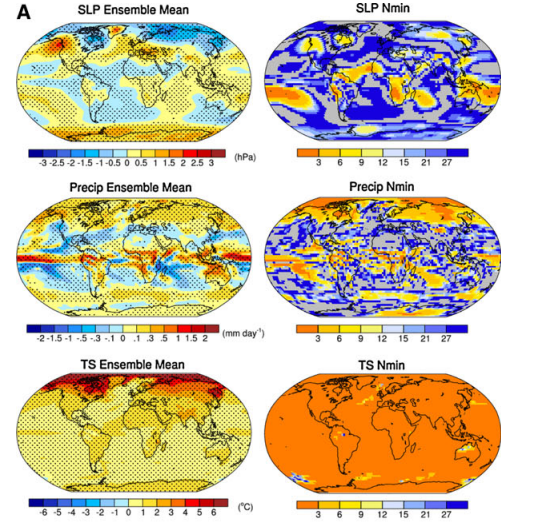
\includegraphics[width=0.8\linewidth]{work/01-variability/figures/EnsembleSenta} 

}

\caption{CCSM3 40-member ensemble (@deser)}\label{fig:EnsembleSenta}
\end{figure}

The climate model ensemble from (\citet{deser}) in more detail. A coupled ocean-atmosphere-land-cryosphere general circulation model (CCSM3) is used. It realistically simulates the main patterns of climate variability, but shows a higher regularity and frequency for ENSO than in nature. The 40-member CCSM3 ensemble uses the T42 version with specific resolutions for the different components and considers the A1B greenhouse gas scenario. The initial conditions for ocean, land and sea ice are identical for each ensemble member and are from 1 January 2000, while the atmospheric conditions vary.
In addition, a 10,000-year control integration of CAM3, the atmospheric component of CCSM3, is used. This integration takes into account recurring seasonal cycles without annual variability based on observations from 1980-2000.
A separate CMIP3 multi-model ensemble was formed for the study, comprising a single integration of 21 models with the SRES-A1B forcing scenario, excluding CCSM3. The climate response was calculated using epoch differences and linear trends for the period 2005-2060. Both methods provide almost identical results. The statistical significance of the results was assessed using a two-tailed Student's t-test.
The left panels of Figure 1a show the ensemble mean epoch difference maps (2051-2060 minus 2005- 2014) for sea level pressure (SLP), precipitation (Precip) and surface temperature (TS) during December-January-February (DJF) for the 40-member CCSM3 ensemble. Hatching indicates areas where the differences are significant at a 95\% confidence level.
After explaining the model and the method, the results are now presented. The ensemble mean response is globally considerable for all three variables. Sea level pressure shows negative values at high latitudes in the northern hemisphere and positive values at mid-latitudes, similarly in the southern hemisphere, but with reversed polarity. These patterns correspond to the northern and southern annular modes (NAM and SAM). The global distribution of SLP changes is consistent with the results of 22 CMIP3 models.
Precipitation shows positive values along the equator and negative values south of it. Subtropics generally have less precipitation, while extratropical regions have more precipitation. The surface temperature is rising everywhere, with stronger warming over land and maximum warming in the Arctic due to the loss of sea ice in autumn.
The right panels of Figure 1a show the minimum number of ensemble members required to detect a significant response. Sea level pressure requires larger ensemble sizes than precip, and surface temperature requires the smallest ensemble sizes. Values for SLP range from less than 6 in the tropics to over 15 in other regions. Precip usually requires fewer members, while TS generally requires less than 3 members, except in some isolated regions. It can also be said that the grey areas indicate the locations where the mean response of the 40-member ensemble is not at the 95\% confidence level.(\citet{deser})

\section{3. Internal variability in the climate system}\label{internal-variability-in-the-climate-system}

The study of internal variability in the climate system is of central importance for understanding the complex interactions and fluctuations within the Earth's climate. Internal variability refers to naturally occurring fluctuations in the climate system that arise independently of external influences such as greenhouse gas emissions, volcanic eruptions or solar variations. This variability can manifest itself on different time scales, from monthly and seasonal fluctuations to decade and century scales.
A prominent example of internal variability is the phenomenon of the North Atlantic Oscillation (NAO), which has a considerable impact on weather and climate conditions in Europe and North America. The NAO influences the temperature and precipitation patterns in these regions through its fluctuations, which in turn can be attributed to the internal dynamics of the circulation systems. The thermohaline circulation also plays a substantial role in internal variability, particularly in the North Atlantic region, where variations in the flow and the associated heat distribution have considerable climatic effects (\citet{latif2022natural}).
The role of internal variability is particularly important for climate research and modelling, as it contributes to considerable uncertainties in climate projections. Models that do not adequately account for this internal variability tend to underestimate or overestimate the variability of the climate system. For example, studies show that the uncertainties in projections of ocean temperatures and ocean currents are influenced by internal variability (\citet{deser}). These uncertainties have a direct impact on the predictability of future climate trends and the planning of adaptation strategies.
The fluctuations in surface temperature and ocean currents observed in the North Atlantic region illustrate the need for precise monitoring and modelling of internal variability processes. This is important in order to distinguish both natural and anthropogenic drivers of climate change and to develop appropriate climate adaptation measures. It is argued that ongoing observation programmes and high model resolutions are necessary to better understand and predict these complex processes (\citet{latif2022natural}).
Internal variability can have both positive and negative effects, depending on the specific climate component and regional characteristics. For example, increased internal variability in the tropics can lead to changes in global atmospheric circulation, which in turn influence climate extremes such as droughts and floods (\citet{deser}).
Understanding these internal processes is therefore crucial for improving the accuracy and reliability of climate models and thus also for developing effective climate change mitigation and adaptation strategies.

\section{3.1 Definition and causes of internal variability}\label{definition-and-causes-of-internal-variability}

Internal variability in the climate system is a central element of climate research and describes fluctuations in the climate that are not caused by external influences such as volcanic eruptions or human activities, but arise from internal dynamics of the climate system itself. The main drivers of this internal variability are the complex interactions between the various components of the climate system, in particular between the atmosphere, oceans, cryosphere and biosphere. Internal variability is the natural variability of the climate system that occurs in the absence of external forcing and includes processes inherent to the atmosphere, ocean and coupled ocean-atmosphere system.
A major cause of internal variability is the thermodynamic coupling between the atmosphere and the near-surface layers of the oceans. This coupling can cause long-lasting climate fluctuations that last for years to decades (\citet{deser}). A prominent example of such variability is the North Atlantic Oscillation (NAO), which is characterised by fluctuations in air pressure between the Icelandic low and the Azores high. These fluctuations have an influence on the weather and climate in the mid-latitudes of the North Atlantic (\citet{latif2009dynamics}).
Another important factor is the wind-driven circulation systems of the oceans, such as the ocean gyre, which can contribute to the Pacific Decadal Oscillation and the Atlantic Multidecadal Oscillation. These processes can be influenced by changes in atmospheric circulation, such as different wind patterns and variations in air pressure (\citet{deser}).
Within the North Atlantic, changes in the thermohaline circulation, also known as the Atlantic Meridional Overturning Circulation (AMOC), play a essential role. This circulation contributes to the distribution of heat within the ocean and is strongly dependent on the salinity and temperature of the seawater. The natural fluctuations of the AMOC can have a considerable impact on the climate of the North Atlantic and lead to multidecadal variations (\citet{latif2022natural}).
The internal variability of the climate system is therefore caused by a variety of mechanisms that operate on different spatial and temporal scales. These mechanisms are often stochastic in nature and can be described by internal dynamical processes such as interactions between ocean and atmospheric wind patterns (\citet{latif2009dynamics}).
In contrast to internal variability, external variability is caused by external drivers; these external factors can influence the climate over longer periods of time. One example of this is changes in solar radiation or volcanic eruptions. In addition, human influences can also play a role, such as greenhouse gas emissons.
To summarise, it can be said that the internal variability in the climate system represents a complex interplay of different factors that include both thermal and dynamic processes. This variability is fundamental to understanding the climate system in all its dynamics and results from the internal interactions of the various climate components. It forms an essential basis for better understanding the uncertainties in climate projections and thus also the planning of adaptation strategies for dealing with climate change.

\section{3.2 Effects of internal variability on climate projections}\label{effects-of-internal-variability-on-climate-projections}

The internal variability in the climate system represents a major uncertainty for climate projections. This variability results from natural processes within the climate system itself and is not caused by external forcing such as greenhouse gases or land-use changes. The internal variability manifests itself on different time scales, from seasonal to multi-decadal, which complicates the interpretation and prediction of future climate conditions.
A key point that illustrates the uncertainties in climate projections is the role of atmospheric circulation. Studies have shown that variations in atmospheric circulation can contribute strongly to uncertainty in climate models (\citet{monerie2020model}). For example, differences in simulated atmospheric dynamics, such as the movement patterns of air masses, contribute essential to the variable amount of precipitation in the Sahel. These uncertainties remain in both older (CMIP5) and newer models (CMIP6) (\citet{monerie2020model}).
Another example of the effects of internal variability is the Atlantic Meridional Overturning Current (AMOC). The AMOC is a large-scale ocean current that transports heat from the tropics to higher latitudes and thus has an influence on regional climate patterns. Studies have shown that the internal variability of the AMOC has been the dominant force since 1900 (\citet{latif2022natural}). Depending on its state, this internal variability can have short-term and long-term effects on the surface temperatures of the North Atlantic and the European climate.
Internal variability is also increased by other factors such as the North Atlantic Oscillation (NAO) and the Atlantic Multidecadal Oscillation (AMO). Fluctuations in these systems can influence the European and North American climate and lead to seasonal to decadal variations in temperature and precipitation (\citet{latif2022natural}).
Furthermore, internal variability complicates policymaking and decision-making as it leads to ranges in climate predictions. This makes accurate predictions difficult and emphasises the need for robust adaptation strategies that consider a variety of scenarios to minimise uncertainties (\citet{tomassini2010uncertainty}).
Finally, it can be stated that internal variability is an important, but often difficult to predict component in climate projections. It strongly influences the uncertainty range of model projections and therefore further studies are urgently needed to better understand the mechanisms of internal variability and to quantify its impact on climate projections more precisely.

\section{4. Application and meaning of climate model ensembles in research}\label{application-and-meaning-of-climate-model-ensembles-in-research}

The use and importance of climate model ensembles in research has grown considerably in recent years. Climate model ensembles are a valuable method for assessing and minimising uncertainties in climate projections. These models make it possible to incorporate the internal variability of the climate system by performing multiple simulations with different initial conditions or model parameters. By using ensemble techniques, the range of possible climate projections can be better understood and the uncertainties arising from internal variability and model specificities can be quantified (\citet{deser}).
However, the role of climate model ensembles goes beyond the mere assessment of uncertainty. They also provide a robust basis for the assessment of climate dynamics under different scenarios and forcing conditions. Ensemble models facilitate the identification of systematic errors in models and enable the assessment of model performance by comparison with observations and other models (\citet{eyring2016overview}). This comparability is particularly important to strengthen confidence in future climate projections and to check the reliability of the models.
In addition, climate model ensembles offer the possibility of analysing the effects of climate change on different spatial and temporal scales. By considering ensembles on a regional scale, researchers can make more accurate predictions about local climate trends and extreme events. This is of particular importance for adaptation to climate change, as it enables decision-makers to develop well-founded and location-specific strategies. For example, modelling can be used to plan agricultural adaptation measures to changing climate conditions by assessing the uncertainties in the projected impacts and using statistical tools such as Monte Carlo simulations (\citet{falloon2014ensembles}).
Another key aspect is the promotion of cooperation within the scientific community. The Coupled Model Intercomparison Project Phase 6 (CMIP6) is an outstanding example that shows how coordinated modelling and data comparison between different research centres help to expand the scientific basis and the validity of climate models (\citet{eyring2016overview}). These collective efforts not only strengthen the quality of the models, but also their ability to respond to the challenges and issues of climate change.
To summarise, climate model ensembles are an indispensable tool in climate research. They help to reduce uncertainty in climate projections, support the development of robust climate predictions and foster deeper collaboration between research centres worldwide. The ongoing development and application of these models will be crucial to better understand the complexities of the climate system and to develop appropriate adaptation strategies.

\section{4.1 Use of climate model ensembles for robust climate predictions}\label{use-of-climate-model-ensembles-for-robust-climate-predictions}

The benefits of climate model ensembles for robust climate predictions are manifold and crucial for the accuracy and reliability of long-term climate projections. These ensembles, which consist of a large number of independent model simulations, make it possible to evaluate and minimise the uncertainties in climate predictions due to internal variability and model-inherent uncertainties.
By using climate model ensembles, the effects of internal variability on future climate projections can be better understood. Internal variability, which is due to natural fluctuations in the climate system, can cause considerable uncertainty in projections (\citet{deser}). Climate model ensembles offer the possibility to quantify these uncertainties by combining a large number of simulations under different initial conditions and with different models. This helps to better map the range of possible future climate states and to increase the robustness of the predictions.
Another advantage of climate model ensembles is the improvement in the statistical representativeness of the climate model outputs. By superimposing many simulations, systematic errors of individual models can be compensated and a more reliable estimate of future climate conditions can be achieved. The probabilistic assessment of future climate trends, as made possible by Bayesian models, ensures that the uncertainties in the model forecasts are adequately taken into account (\citet{smith2009bayesian}).
In addition, climate model ensembles make valuable contributions to the production of regional and seasonal climate predictions, which are of central importance for adaptation strategies at the local level. For example, high-resolution climate models within an ensemble can be used to project specific regional climate changes in more detail (\citet{croce2021enhancing}). This is particularly important for regions that are strongly affected by specific climate extremes, such as the Mediterranean region, where extreme temperature and precipitation events need to be intensively analysed (\citet{croce2021enhancing}).
By considering different emission scenarios in the simulations, the range of possible future climate states can also be covered. This is essential in order to plan and implement adaptive measures that can react flexibly to different climatic developments. A multi-model ensemble thus enables a more robust and comprehensive consideration of climate risks and contributes to improved strategic decision-making (\citet{deser}; \citet{smith2009bayesian}).
To summarise, climate model ensembles provide an indispensable basis for making well-founded and reliable climate predictions. They not only enable a realistic assessment of uncertainties, but also support the development of specialised and regionally adapted climate adaptation strategies. This makes them an essential tool in modern climate research and planning.

\section{4.2 Application examples: regional and seasonal climate trends}\label{application-examples-regional-and-seasonal-climate-trends}

Climate model ensembles play a crucial role in producing robust regional and seasonal climate predictions. By using a multi-model approach, uncertainties can be minimised and the accuracy of projected climate changes can be increased. An illustrative example of this is the study of long-term spatiotemporal variability and trends in extreme rainfall and temperatures in Bangladesh, which can have an impact on rice production (\citet{mainuddin2022long}). The analysis shows regional variations in climate trends, such as the decrease in precipitation in specific regions and the marked rise in temperature, which could substantially affect agricultural yields.
Another example is the use of EURO-CORDEX RCMs and HighResMIP GCMs to analyse the daily precipitation distribution in Europe. These high-resolution models provide an improved representation of precipitation patterns compared to older CMIP5 models. In particular, the PRIMAVERA GCMs show precipitation distributions that are closer to observations in many European regions than the results of the EURO-CORDEX RCMs (\citet{demory2020european}). Such regional climate models are particularly useful for simulating complex topographical and coastal areas more precisely, which is crucial for predicting extreme weather events, for example.
Seasonal trends are of particular interest in climate research as they have a direct impact on agricultural productivity and water resources. Analyses of climate models show that intensified precipitation and longer dry periods have different regional effects. For example, some models show a tendency to overestimate winter rainfall and underestimate summer rainfall, which can be partially corrected by finer grid resolutions (\citet{demory2020european}). Such seasonal discrepancies must be taken into account when planning and adapting agricultural and water management strategies in order to increase resilience to climate change.
The importance of climate model ensembles is emphasised by the combined use of regional and global models. These models make it possible to understand and project the climate at different scales, which is particularly valuable for assessing potential climate risks in specific regions. In this way, the results of this modelling help to develop early warning systems and adaptation strategies that can counter the effects of extreme weather events and support long-term planning (\citet{falloon2014ensembles}). Overall, these application examples illustrate that climate model ensembles are an indispensable tool for analysing and predicting regional and seasonal climate trends. They provide a sound basis for scientifically sound decision-making processes and adaptation planning in the face of advancing climate change.

\section{5. Conclusion}\label{conclusion}

The relationship between natural variability and climate modelling is a central aspect of climate science. Natural variability refers to the natural fluctuations in the climate system caused by internal processes such as El Niño/La Niña, volcanic activity or solar cycles. These fluctuations occur independently of human influences and can affect the climate in the short and medium term. Climate models attempt to take both these natural and anthropogenic (man-made) factors into account in order to provide a realistic simulation of the climate. They use historical data and physical laws to simulate and predict natural climate fluctuations.
Natural variability can cause short-term fluctuations in temperature and precipitation that differ from the long-term trends due to climate change. Climate models show that natural variability can have a major impact on regional climate patterns in the coming decades, even if the long-term trend is dominated by anthropogenic climate change. Scientists compare the results of climate models with historical climate data to assess the accuracy of the models. Models that can correctly simulate natural variability are better able to predict future climate changes.
Despite the progress made in modelling, there are still challenges. The complexity of the climate system and the large number of influencing factors make modelling natural variability a challenge. Moreover, uncertainties regarding future natural events and their impact on the climate system pose an additional difficulty. Overall, natural variability is an integral part of climate modelling, and understanding its mechanisms and influences is crucial for the accuracy of climate projections.

\chapter{Standard Precipitation Evapotranspiration Index}\label{spei}

\emph{Author: Author}

\emph{Supervisor: Henri Funk}

\emph{Suggested degree: Bachelor}

\section{Definition}\label{definition}

The SPEI is a statistical indicator that shows dry and wet periods on the basis of the climatic water balance (total precipitation minus total potential evaporation). It captures water deficits or surpluses on the land surface better than the Standardised Precipitation Index (SPI), which focuses solely on precipitation. The potential evaporation can be based on the so-called FAO grass evaporation, which takes into account radiation, air temperature, relative humidity and wind speed over a standard grass area. The time series is broken down into 12 monthly frequency sums, to each of which a cumulative log-logistic distribution is fitted. This is transformed into a corresponding cumulative standard normal distribution, the abscissa value of which - referred to as SPEI - allows simple assignment to probability classes.
\citet{vicente}

\chapter{Compound events}\label{ce}

\emph{Author: Author}

\emph{Supervisor: Henri Funk}

\emph{Suggested degree: Master}

In climate research, a compound event refers to the combination of multiple extreme weather or climate events occurring simultaneously or successively, leading to significant impacts on the environment, society, or economy. These events can be related either through meteorological factors (e.g., heatwaves and drought occurring together due to a prolonged high-pressure system) or through their impacts (e.g., heavy rainfall and storm surge combining to cause more severe flooding). The complexity of compound events lies in their interconnectedness and the way they can exacerbate each other's effects, often in a nonlinear manner, making them more challenging to predict and manage than individual extreme events.

\section{Example: Hot and Dry Events}\label{example-hot-and-dry-events}

Consider a scenario where a region experiences both extreme heat and an extended period of low precipitation simultaneously. In this example, the compound nature of the hot and dry events creates a cascade of impacts that are more severe than what would be expected if these events occurred independently. The interplay between the heat and drought amplifies the consequences, underscoring the importance of understanding and managing compound events in the context of climate change and variability.
\citet{zscheischler}

\chapter{Assymetric bivariate Copulas for compounds}\label{ac}

\emph{Author: Author}

\emph{Supervisor: Henri Funk}

\emph{Suggested degree: Master}

In compounds, particularly in environmental and hydrological contexts, bivariate relationships can be used to study how two different environmental factors, such as temperature and precipitation, interact with each other. These relationships are critical for modeling the joint behavior of these variables, which can be essential for predicting weather events, designing structures, or managing natural resources.

In the study of environmental and hydrological systems, recognizing and accurately modeling the asymmetry in bivariate relationships is crucial for making reliable predictions and informed decisions. Techniques such as copulas, are often used in this context to model and analyze these complex and dependencies effectively. To model the asymmetry in dependencies, Archimax could be used.

\citet{charpentier}
\citet{bacigal}

\chapter{Teleconnections North Atlantic Oscillation}\label{nao}

\emph{Author: Pamela Sorelle Tueam}

\emph{Supervisor: Henri Funk}

\emph{Suggested degree: Bachelor}

\section{Abstract}\label{abstract-1}

The concept of teleconnections in climate science refers to climate anomalies or patterns that are related across large distances, often thousands of kilometers apart. Teleconnections represent atmospheric interactions that link weather and climate conditions in one region of the globe with those in another, often through the movement and behavior of large-scale atmospheric wave patterns (\citet{feldstein2017}). These connections are crucial for understanding regional climate variations, predicting weather patterns, and assessing climate change impacts. One prominent example of a teleconnection pattern in the Northern Hemisphere is the North Atlantic Oscillation (NAO). This oscillation plays a significant role in influencing the climate over the North Atlantic region. Its impacts are observed in various climate elements, including temperature, wind speed and direction, storm and precipitation, as well as ocean and sea ice dynamics. \(\\\)
This chapter explores various methods for defining and analyzing the North Atlantic Oscillation (NAO), following the framework established by \citet{hurrell2010}. These methods include one-point correlation map, Empirical Orthogonal Function (EOF) analysis, and cluster analysis. Additionally, we present the long-term trends of the NAO using the NAO Index. Through a detailed examination of these approaches, we aim to provide a better understanding of the spatial and temporal characteristics of the NAO. Such understanding is important for improving climate models, enhancing weather prediction accuracy, and developing robust climate change adaptation and mitigation strategies. Furthermore, by assessing the NAO's influence on temperature, wind patterns, storm activities, and oceanographic conditions, this chapter contributes to a deeper comprehension of how large-scale atmospheric phenomena shape our climate system.

\section{Introduction}\label{introduction-1}

The North Atlantic Oscillation (NAO), one of the most prominent and recurrent teleconnections over the Northern Hemisphere, is characterized by a redistribution of atmospheric mass at sea level between the Icelandic Low and the Azores High (\citet{hurrell2010}). It dictates climate variability from the eastern seaboard of the United States to Siberia and from the Arctic to the subtropical Atlantic, especially during boreal winter. Fluctuations from one phase of the NAO to another result in significant variations in the average wind speed and direction over the Atlantic, as well as in the transport of heat and moisture between the Atlantic and neighboring continents. This also affects the intensity and number of storms, their paths, and associated weather conditions (\citet{hurrell2003}). Especially during the months of December to March, the NAO is responsible for much variability of weather over the North Atlantic region. Thus, the NAO influences weather and climate conditions across the North Atlantic region and beyond, affecting winter temperatures and storm tracks. \(\\\)
In this chapter, our primary focus will be on exploring the spatial and temporal characteristics of the NAO. We will begin by discussing common methods used to define it, such as the one-point correlation map, which helps to identify the NAO by regions of positive and negative correlations. Additionally, we will employ the EOF analysis to discern the dominant patterns of variability associated with the NAO, and utilize the cluster analysis to identify distinct atmospheric patterns with similar pressure characteristics. Furthermore, we will analyze the NAO Index to observe its variations over long periods. Finally, we will investigate the impacts of the NAO on various climate factors including temperature, wind speed and direction, precipitation patterns, storm activities, oceanic conditions, and sea ice dynamics.

\section{The spatial and temporal structure of the NAO}\label{the-spatial-and-temporal-structure-of-the-nao}

Understanding NAO requires a comprehensive understanding of its spatial and temporal characteristics. To analyze these aspects, we will review established methods commonly employed for defining or identifying NAO patterns. These methods include the one-point correlation map, the EOF analysis for its spatial structure, as well as cluster analysis. For its temporal structure, we will focus on the NAO index. These methods are used in the paper of (\citet{hurrell2010}) and the data used in his paper go up to 2006. The idea is to reproduce these on new data up to 2024 and see if the NAO patterns remain similar.

\subsection{Data}\label{data}

Monthly geopotential height at 500 hPa (Z500) and mean sea level pressure (MSLP) data are used in this chapter. The monthly geopotential height at 500 hPa were obtained from the ERA5 reanalysis dataset for global climate and weather (\citet{geopotential2023}).
Mean sea level pressure data used here were also sourced from the ERA5 reanalysis (\citet{mean_sea_level2023}) dataset. For both monthly geopotential height and mean sea level pressure, only data from the Northern Hemisphere specifically within the coordinates 20°-70°N and 90°W-40°W, were extracted. Considering that the NAO is responsible for much variability of weather in boral winter over the Northern Hemisphere, the period from December to March (DJFM) was selected for this analysis. The time series used consist of 84 DJFM seasons from 1940-2024. The data used to examine the NAO Index were collected from the National Center for Atmospheric Research (NCAR). This dataset includes station-based NAO index data of 159 DJFM seasons spanning from 1864 to 2023 (\citet{nao_index_2003}). To examine the pattern of variability we need to compute the anomalies which are calculated by subtracting time means, computed for each calender month from the data for individual year-months. These anomalies form the basis for all methods described in this chapter.

\subsection{One-point correlation maps}\label{one-point-correlation-maps}

One way to define the NAO is through conceptually simple one-point correlation map, identifying the NAO by regions of maximum negative correlation over the North Atlantic. For these one-point correlation we will focus on the methods described by \citet{athanasiadis2009} and by \citet{wallace1981} in their respective papers. \(\\\)
One-point correlation correlates a variable at a specific location with the same variable at other locations. Given a field of data, we compute the correlation coefficient between the base point - referred to as the center of action - and each other points. The center of action is a specific location defined by latitude and longitude. The resulting correlation values generate a map that identifies the NAO by regions of positive and negative correlation. In this analysis, we use monthly geopotential heights data at 500 hPa for winter season December-March from 1940 to 2024. Anomalies are calculated by subtracting geopotential height time means, computed for each calendar month from the data for individual geopotential height year-months (\citet{wallace1981}, 790). \(\\\)
The correlation coefficient for a given center of action is calculated using the Pearson's linear correlation coefficient at every point as follows:

\(r_{i} = \frac{Cov(X_{i}, Y_{i})}{\sqrt{Var(X)Var(Y)}}\)

where X and Y are time series of contemporaneous observations, \([(x_{i}, y_{i}); i = 1, 2, . . . N]\), where we fix one of the data points, say, X, at the center of action and compute the correlation over all Y. Covariance and variance are denoted as Cov and Var, respectively (\citet{athanasiadis2009}, 3721). \(\\\)
Figure \ref{fig:CorrelationPamela} illustrates the corresponding one-point correlation map for the NAO pattern. The reference point that has been chosen is located in Iceland at 65°N and 18°W. The correlations are calculated for all points belonging to the Northern Hemisphere (20-70°N, 90°W-40°E).
As we can see on the figure the map is characterized by more or less elliptical regions where correlation coefficients can be positive or negative, surrounding each base grid point. The size of these regions provides an indication of the horizontal scale of the anomalies, particularly near the base grid points (\citet{wallace1981}, 790).
The identifying dipole patterns located at the Icelandic Low and Azores High, reflect the NAO signature based on the chosen reference point. The color gradients on the figure indicate the strength of the correlation, with blue representing negative correlations and yellow to red representing positive correlations. \(\\\)
As implications, regions with strong positive correlations experience atmospheric conditions similar to Iceland (the center of action). These areas may share similar temperature anomalies. For instance, if the region of the center of action experiences warmer-than-average temperatures during high NAO phase, positive correlated regions might also experience similar warmth temperatures. We will also have similar precipitation patterns (if it is drier than the nearby regions may also be similar dry). Conversely, the region with negative correlations such as the anticorrelation center at Azores, will exhibit opposite conditions, including temperature contrasts (warmer vs.~cooler) and differing precipitation patterns (wetter vs.~drier).

\begin{figure}

{\centering 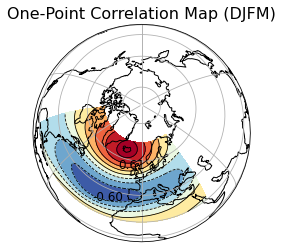
\includegraphics[width=0.5\linewidth]{work/05_nao/figures/OnePointCorrelation} 

}

\caption{One-point correlation map of 500 hPa geopotential height for boreal winter (December-March) over 1940-2024. The reference point is 65°N, 18°W. Negative correlation coefficients are in blue and the lines are dashed.}\label{fig:CorrelationPamela}
\end{figure}

\subsection{EOF Analysis}\label{eof-analysis}

The second method is the Empiriacal Orthogonal Function (EOF) analysis, also known as Principal Component Analysis (PCA). EOF analysis is commonly used to identify and analyze dominant patterns of variability in spatial and temporal datasets. The EOFs of a dataset are simply the eigenvectors of the covariance matrix of the dataset, which provide maximal data compression (\citet{wilks2011}). The method reduces a dataset with many variables to a smaller set of new variables, which are linear combinations of the original ones, chosen to capture the maximum possible variability of the original data (\citet{wilks2011}). Given multiple observations of a (K × 1) data vector \(\textbf{x}\), PCA finds (M x 1) vector \(\textbf{u}\), which are linear combinations of the elements of \(\textbf{x}\) and capture most of the information from the original data (\citet{wilks2011}). The steps by performing the EOF are as follows:

\begin{itemize}
\tightlist
\item
  Collection of the dataset: We used the mean sea level pressure (MSLP) data for boreal winter DJFM over 84 years from 1940 to 2024.
\item
  Calculation of the anomalies: Anomalies are calculated by subtracting the MSLP time means, computed for each calendar month from the data for individual MLSP year-months.
\item
  Formation of the Covariance Matrix as we want to analyze the variance and patterns in the data.
\item
  Performance of the eigenvalue decomposition: The covariance matrix is decomposed using eigenvalue decomposition to obtain the eigenvalues and eigenvectors. The eigenvectors represent the spatial patterns, and the eigenvalues indicate the amount of variance explained by each EOF.
\item
  The first principal component, \(u_{1}\) is obtained as the projection of the anomalies vector onto the first eigenvector \(\textbf{e}_{1}\) \(\textbf{u}_{1} = \textbf{e}_{1}^{T} = \sum_{k= 1}^{K} e_{k, 1}x_{k}^{'}\). This first EOF/PC explains the most variance, followed by the second, and so on (\citet{wilks2011}).
\end{itemize}

Computing the EOFs allows for comparison with the results of the one-point correlation analysis. While correlation analysis focuses on the variability relative to the primary center of action of specific teleconnections, EOF analysis is not centered on specific points. The loading at any two points are not solely determined by the temporal correlation between the time series at those points (\citet{athanasiadis2009}, S 3724). Furthermore, EOF analysis is not explicitly designed to highlight regional patterns of strong correlation. Instead, EOF analysis sequentially identifies the leading patterns that explain the most variance within the analyzed dataset (\citet{athanasiadis2009} S 3724). Therefore, values of the same sign at two different spatial points in an EOF do not necessarily imply a significant correlation between those two points.

Figure \ref{fig:EofPamela} illustrates the leading eigenvectors of the cross-covariance matrix calculated from seasonal (4-month average) MSLP anomalies in the North Atlantic sector (20°-70°N; 90°W-40°E). Since the eigenvectors are, by definition, structured to explain maximum variance, it is expected that the center of actions of the leading EOFs will coincide with the regions of strongest variability. Although EOF patterns are not exactly identical to the one-point correlation map, there is a noticeable similarity between the two. Both correlation map and EOF analysis consistently illustrate the distinct behavior of variability across different time scales. During the winter season (December-March), the NAO accounts for more than one-third (35.8\%) of the total variance in SLP over the North Atlantic and appears with a slight northwest-to-southeast orientation.

\begin{figure}

{\centering 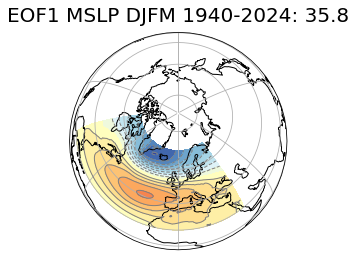
\includegraphics[width=0.6\linewidth]{work/05_nao/figures/EOF1} 

}

\caption{Leading empirical orthogonal function (EOF 1) of the seasonal mean sea level pressure anomalies in the North Atlantic sector (20°–70°N, 90°W–40°E), and the percentage of the total variance it explains. The data cover the period of 1940–2024.}\label{fig:EofPamela}
\end{figure}

\subsection{Cluster Analysis}\label{cluster-analysis}

Another method to examine the dynamical signature of interannual variability in the North Atlantic is the cluster analysis. This non-linear approach groups similar data points into clusters based on their similarities, and is used here to identify distinct atmospheric patterns with similar pressure characteristics. It is applied to 84 years of monthly MSLP data from December to March using procedures based on a clustering algorithm. The algorithm groups in this case the monthly MSLP data into a small number of representative states (or regimes) according to an objective criterion of similarity.
Given a prescribed number of clusters \(k\), the goal of the algorithm is to find a partition \(P\) of the data points into \(k\) clusters \(C_{1}, C_{2}, …, C_{k}\) that minimizes the sum of the variances within the clusters, expressed as (\citet{michelangeli1995}): \[W(P) = \sum_{j= 1}^k \sum_{x \in C_{j}} d^2(X, Y_{j})\] where \(Y_{j}\) is the centroid cluster \(C_{j}\) and \(d(X, Y)\) represents the Euclidean distance between two points X and Y as a measure of similarity. The global minimum of the function \(W(P)\) therefore corresponds to a partition that achieves the best separation of data points. The dynamic cluster algorithm defines iterative partitions \(P^{(n)}\) for which \(W(P^{(n)})\) decreases with n and eventually converges to a local minimum which generally differs from the global one. This algorithm thus provides the optimal \(k\) number of clusters to be retained (\citet{michelangeli1995}, S 1241).
The steps by performing the cluster Analysis are:

\begin{itemize}
\tightlist
\item
  Data collection and anomalies calculation.
\item
  Selection of a clustering algorithm: In this case the k-means clustering is used.
\item
  Determination of the optimal number of clusters.
\item
  Application of the algorithm: Assign each monthly SLP data to a cluster with each cluster representing a distinct atmospheric regime or pattern.
\end{itemize}

The clustering algorithm applied over the Atlantic domain (20°--70°N; 90°W--40°E) identifies four winter climate regimes Figure \ref{fig:RegimesPamela}. The clustering partition yields the optimal \(k = 4\) number of significant winter climate regimes subsequently represented by the cluster centroid. Two of these clusters correspond to the negative and positive phases of the NAO and are characterized by a zonally elongated meridional pressure dipole between the Icelandic Low and the Azores High. The third regime exhibits a zonal pressure dipole between Greenland and Scandinavia (the ``Blocking'' regime) with a clear southeastward extension of low-pressure anomalies toward the Iberian Peninsula. The fourth regime displays a strong anticyclonic ridge (RDG) over western Europe (the ``Atlantic Ridge'' regime) (\citet{hurrell2010}).

\begin{figure}

{\centering 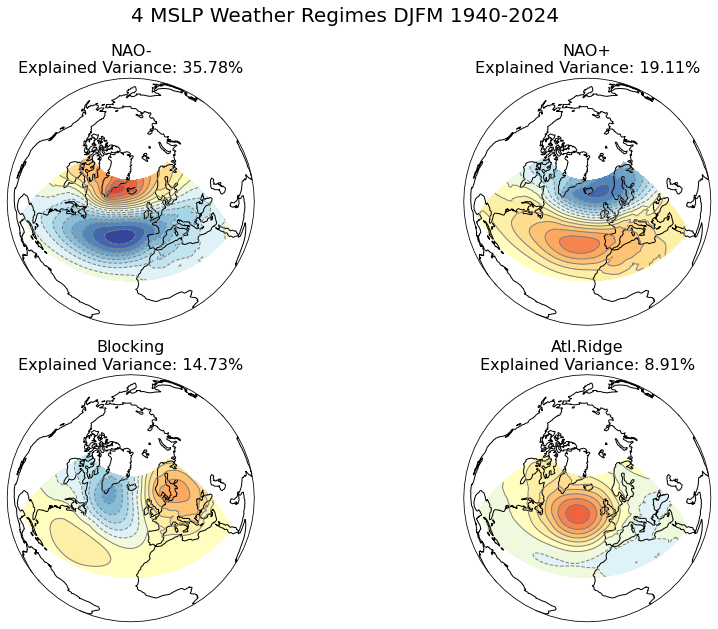
\includegraphics[width=0.7\linewidth]{work/05_nao/figures/ClusterAnalysis} 

}

\caption{Boreal winter (December–March) climate regimes in sea level pressure (hPa) over the North Atlantic domain (20°–70°N, 90°W–40°E) using monthly data over the period from 1940 to 2024. The percentage on each panel expresses the explained variance of each cluster.}\label{fig:RegimesPamela}
\end{figure}

\subsection{NAO positive and negative Index}\label{nao-positive-and-negative-index}

The most modern NAO indices are derived either from the simple difference in surface pressure anomalies between selected northern and southern locations, or from the PC time series of the leading Empirical Orthogonal Function (EOF) of the sea level pressure (SLP) field (\citet{hurrell2010}). Although the NAO is observable throughout the year, it is most pronounced during winter, accounting for over one-third of the total variance in the SLP field over the North Atlantic (\citet{hurrell1997}, 305). (\citet{hurrell1997}) defined a simple index of the NAO as the difference between the normalized mean winter (December--March) SLP anomalies at Lisbon, Portugal and Stykkisholmur, Iceland.

Figure \ref{fig:IndexPamela} illustrates the positive and negative index of the NAO from 1864 to 2023. The average winter sea level pressure data at each station were normalized by division of each seasonal pressure by the long-term mean (1864--2023) standard deviation. Positive values of the index are in red and negative values in blue. The NAO index, as depicted in Figure \ref{fig:IndexPamela}, exhibits a well-defined oscillation. However, several periods exist where the NAO index remained in one phase over multiple winters, such as from 1903 to 1914 (positive phase), from 1915 to 1919 (negative phase), from 1958 to 1971 (negavite phase, excluding 1961 and 1967), and from 2014 to 2020 (posivite phase). On this figure of the NAO index \ref{fig:IndexPamela} we can notice that there is little evidence for the NAO to vary on any preferred time scale. Significant changes can occur from one winter to the next, as well as from one decade to another.\(\\\)

\begin{figure}

{\centering 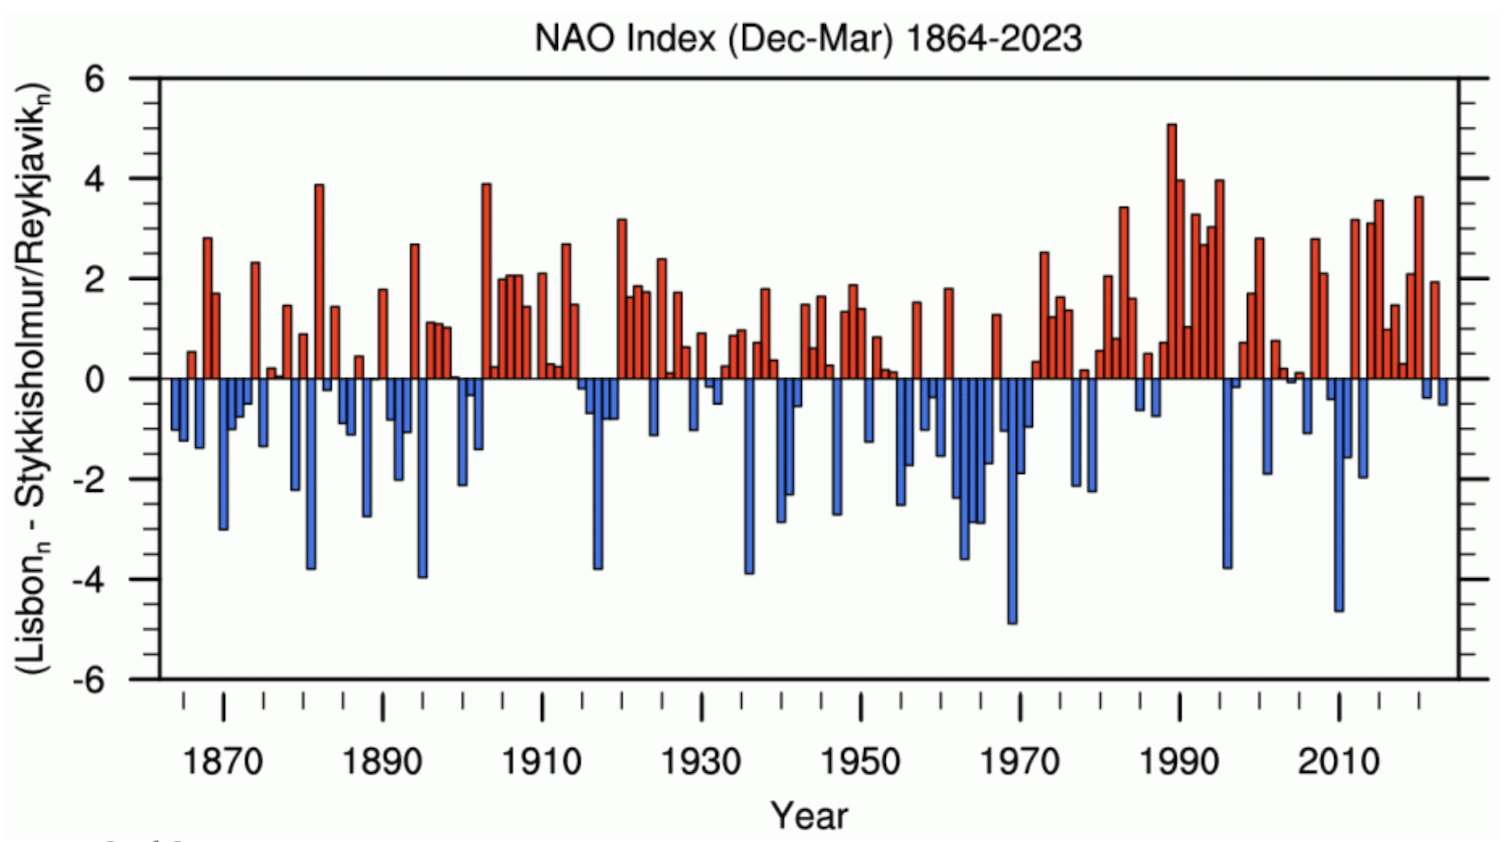
\includegraphics[width=0.8\linewidth]{work/05_nao/figures/NAOIndex} 

}

\caption{Normalized indices of the mean winter (December–March) NAO constructed from sea level pressure data. The index is based on the difference of normalized sea level pressure between Lisbon, Portugal and Stykkisholmur/Reykjavik, Iceland. The average winter sea level pressure data at each station were normalized by division of each seasonal pressure by the long-term mean (1864–2023) standard deviation. The indicated year corresponds to the January of the winter season (e.g, 1990 is the winter of 1989/1990)}\label{fig:IndexPamela}
\end{figure}

The NAO is in a positive phase when both Icelandic low-pressure center and the high-pressure center at the Azores are stronger than the average (figure \ref{fig:phasePamela}). During the positive NAO phase, the increased difference in pressure between these two regions results in a stronger Atlantic jet stream and a northward shift of the storm track. Consequentlly, northern Europe experiences increased storminess, higher precipitation, and warmer-than-average temperatures due to the air masses that arrive from lower latitudes. At the same time, southern Europe experiences decreased storminess and below-average precipitation. In eastern North America, the positive phase of the NAO generally brings higher air pressure, a condition associated with fewer cold-air outbreaks and decreased stormisses (\citet{hurrell2010}).

Conversely, the NAO is in a negative phase when both the Icelandic low and Azores high are weaker than average. During the negative NAO phase, the Atlantic jet stream and storm track have a more west-to-east orientation. This results in decreased storminess, below-average precipitation, and lower-than-average temperatures in to northern Europe. Conversely, southern Europe experiences increased storminess, above-average precipitation, and warmer-than-average temperatures. In eastern North America, the negative phase of NAO generally brings lower air pressure, a condition associated with stronger cold-air outbreaks and increased storminess (\citet{hurrell2010}).

\begin{figure}

{\centering 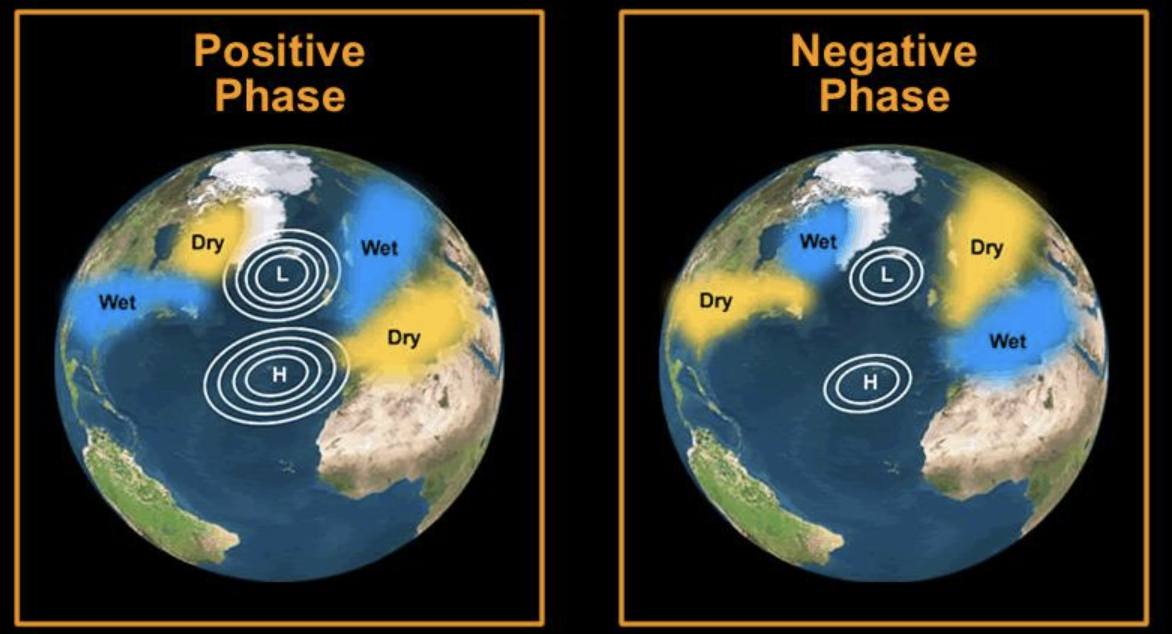
\includegraphics[width=0.7\linewidth]{work/05_nao/figures/NAOPhase} 

}

\caption{Positive and negative phase of the North Atlantic Oscillation. Image from @NAO\_phase2013}\label{fig:phasePamela}
\end{figure}

\section{The Implications of the North Atlantic Oscillation}\label{the-implications-of-the-north-atlantic-oscillation}

The NAO plays a critical role in shaping climate patterns across the North Atlantic and surrounding areas. Changes in its spatial and temporal structures can lead to significant variations in temperature, precipitation, and weather extremes, influencing ecosystems, human activities, and natural resources.

\subsection{Temperature, wind speed and direction}\label{temperature-wind-speed-and-direction}

During the positive phase of the North Atlantic Oscillation (NAO), the atmospheric pressure difference between the Icelandic low and the Azores high intensifies. This results in a stronger-than-usual westerly flow across the North Atlantic during the winter months. Consequently, relatively warm, and moist maritime air is transported over much of Europe and extends across Asia (\citet{hurrell2003}). This influx of warm air can lead to milder winter conditions across the continent, often resulting in higher temperatures (\citet{hurrell2003}). Meanwhile, while stronger northerly winds over Greenland and northeastern Canada transport cold air southward leading to a decrease in land temperatures in the northwest Atlantic (\citet{hurrell2003}). The cold air intrusions can lead to harsher winter conditions in parts of eastern Canada and the northeastern United States. \(\\\)
Additionally, the stronger clockwise circulation around the subtropical Atlantic high-pressure center during this phase of the NAO significantly impacts other regions. In North Africa and the Middle East, this results in cooler-than-average temperatures due to the altered wind patterns. In contrast, parts of North America experience warmer conditions as the strengthened high-pressure system influences the weather patterns across the continent (\citet{hurrell2003}).

\subsection{Storm and precipitation}\label{storm-and-precipitation}

NAO signals can also be found in winter precipitation and storm over the North Atlantic.During the positive phase of the NAO, storm activities in the Atlantic shift northeastward. This means there are more intense and frequent storm activities from southern Greenland across Iceland into northern Europe, and slightly less storm activities from the Azores across the Iberian Peninsula and the Mediterranean (\citet{hurrell2010}). Furthermore, the positive phase is typified by more intense and frequent storms in the vicinity of Iceland and the Norwegian Sea. During the NAO-, a weak subtropical high and a weak Icelandic Low dominate, resulting in a reduced pressure gradient and fewer, weaker winter storms with a more west-east trajectory, while moist air is brought into the Mediterranean and cold air into northern Europe (\citet{rousi2020}).
\(\\\)
Changes in the mean flow and storminess associated with oscillations in the NAO index lead to significant changes in the transport and convergence of atmospheric moisture, impacting the distribution of evaporation and precipitation (\citet{hurrell2010}). These results in drier conditions of this magnitude are observed over central and southern Europe, the Mediterranean, and parts of the Middle East, while more precipitation than normal occurs from Iceland through Scandinavia (\citet{hurrell2010}).

\subsection{Ocean and Sea Ice}\label{ocean-and-sea-ice}

Another implication of the NAO mentioned by \citet{hurrell2010} is its impact on ocean and sea ice. SST and NAO strength fluctuate together, with the main pattern of SST variability in boreal winter forming a tri-polar structure: a cold anomaly in the subpolar North Atlantic, a warm anomaly in mid-latitudes, and a cold anomaly in subtropical regions (\citet{hurrell2010}). These SST anomalies are driven by changes in surface wind and air-sea heat exchanges related to NAO variations. Persistent SST anomalies over longer periods also relate to consistent anomalous SLP patterns, including the NAO, reflecting the ocean's response to long term atmospheric variability.
The reduction of the Arctic Sea ice is one of the most prominent indicators of climate change. less compact ice in high NAO winters plays an important role in the reduction of summer sea ice extent in high NAO years. In winter, the stronger wind in high NAO years drives more ice away from the Eurasian coastal region, suppressing sea ice buildup there (\citet{hurrell2003}).

\section{Conclusion}\label{conclusion-1}

In this chapter we have presented the NAO as the dominant mode of regional climate variability over the Northern Hemisphere, focusing particularly on common methods used to identify its spatial and temporal structure. These methods, although they are different, each have their strengths and limitations.
One point correlation map is easy to implement and interpret providing clear insight into how the chosen center of action is related to the variability at other locations. However, the result heavily depends on the choice of the center of action. Selecting a different center may not well capture the full spatial pattern of the NAO. EOF analysis captures the dominant patterns of variability in a dataset and provides a quantitative measure of how much variance a pattern explains. But it assumes linear relationships and might not capture non-linear features of the NAO. Cluster Analysis is effective at identifying distinct patterns and regimes including non-linear and non-stationary features, but it is computationally intensive and requires careful selection of clustering parameters. Additionally, interpreting the results can be challenging if the patters are not well separated.

As we have seen, the NAO is a significant climatic driver in the North Atlantic region, influencing temperature, wind speed and direction, precipitation, storm tracks, ocean and sea ice, particularly over Europe and North America. Its variability poses challenges and opportunities for understanding and predicting weather and climate impacts in affected regions. Understanding the implications of the NAO for climate change is essential for developing adaptive strategies to deal with the resulting implications on weather patterns and sea ice.

By improving climate models, and implementing robust adaptation plans, we can better address the challenges posed by NAO-induced climate variability. Predicting the future behavior of the NAO in a changing climate is challenging due to the complexity of the interactions between the atmosphere, oceans, and sea ice. Enhanced climate models that incorporate these interactions are crucial for reducing uncertainties and improving forecasts. Despite the strong influence of the NAO, many open issues remain about which climate processes govern NAO variability, how the phenomenon has varied in the past or will vary in the future, and to what extent it is predictable. External factors, such as the rise in greenhouse gas emissions, have a significant impact on the recent patterns of the NAO (\citet{gillett2003}). Research indicates that higher greenhouse gas concentrations are associated with alterations in atmospheric circulation, which may result in more frequent occurrences of positive NAO phases (\citet{gillett2003}). Understanding these shifts is essential for developing strategies to mitigate and adapt to the climate change effects influenced by the NAO (\citet{gillett2003}).

\chapter{Low Flow Events}\label{lfe}

\emph{Author: Author}

\emph{Supervisor: Henri Funk}

\emph{Suggested degree: Bachelor}

Low flow events in hydrology refer to periods when water flow in rivers, streams, or creeks falls below a critical threshold, often leading to various ecological, economic, and social impacts. These events can result from prolonged periods of below-average precipitation, increased water usage, or changes in land use that affect the hydrological cycle. Low flow conditions can compromise water quality, reduce water availability for agricultural, industrial, and domestic uses, and disrupt aquatic ecosystems.

\section{Concept of Extremeness by Return Periods}\label{concept-of-extremeness-by-return-periods}

The ``extremeness'' of hydrological events, including low flow conditions, is often characterized by return periods. A return period, also known as a recurrence interval, is a statistical measure used to estimate the frequency at which a certain intensity of an event (e.g., flow rate, rainfall amount) is likely to be equaled or exceeded. It is typically expressed in years.

\begin{itemize}
\tightlist
\item
  \textbf{Definition}: The return period is calculated based on historical data and is intended to provide an estimate of the likelihood of experiencing an event of a certain magnitude or greater within any given year. For example, a 100-year return period for a low flow event means that, on average, the flow rate is expected to fall to that level or lower once every 100 years. This does not imply the events will occur exactly 100 years apart but rather conveys a 1\% chance of occurrence in any given year.
  \citet{du}
\end{itemize}

\chapter{Statistical streamflow modelling}\label{sm}

\emph{Author: Lennart Marx}

\emph{Supervisor: Henri Funk}

\emph{Degree: Master}

\section{Abstract}\label{abstract-2}

This study evaluates and compares the performance of Long Short-Term Memory (LSTM) networks and Temporal Fusion Transformers (TFT) in forecasting streamflows for up to seven day ahead forecasts, using historical streamflow data alongside precipitation and temperature as covariates. Freely available data published by the bavarian hydrological authority from the Regen river in Bavaria, Germany, was used in conjunction with meteorological data from the ERA5 reanalysis dataset. River basins are defined via the HydroRIVERS and HydroBASINS dataset to obtain the area over which precipitation is aggregated. Results indicate that while both models face challenges in predicting extreme values, TFT maintains more consistent accuracy over longer forecast horizons while pure LSTM model's predictions decline sharply in performance with increasing lead times.

\section{Introduction}\label{introduction-2}

Streamflow forecasting plays a crucial role in water resource management, particularly in flood prediction. As climate change intensifies extreme weather events and alters precipitation patterns, accurate streamflow forecasts have become increasingly important for mitigating flood risks by providing information about the timing and magnitude of potential flood events.This knowledge enables authorities to implement timely flood control measures, operate reservoirs effectively, and issue early warnings to vulnerable communities. As flooding remains one of the most common and destructive natural disasters, especially in developing countries, improved forecasting capabilities can significantly reduce the human and economic toll of these events. (\citet{Nearing2024})

Hydropower is the dominant source of renewable energy, accounting for 16\% of the world's electricity output and 62\% of renewable electricity generation (\citet{hess-26-2431-2022}). Precise streamflow predictions can be beneficial in optimizing reservoir operations. \citet{hess-26-2431-2022} show that this is the case for 94\% of all analyzed dams dependent on forecasting ability and reservoir characteristics.

A streamflow refers to the flow of water in rivers, streams or other water bodies, originating from precipitation, melting snow, and groundwater discharge. It is typically measured in cubic meters per second (m³/s).

In recent years, machine learning techniques have emerged as powerful tools for forecasting in various domains, including hydrology. Traditional hydrological models often rely on extensive datasets and intricate physical parameters, which can be challenging to obtain and process. In contrast, machine learning models such as Long Short-Term Memory (LSTM) networks offer an alternative approach by learning patterns directly from historical data.

This study aims to evaluate and compare the performance of LSTM and TFT models in forecasting streamflows up to seven days ahead. By incorporating precipitation and temperature as future known covariates alongside historical streamflow data, this work seeks to determine the effectiveness of these models in predicting streamflows.

\section{Data}\label{data-1}

\subsection{Preperation}\label{preperation}

The streamflow data is gathered from the bavarian hydrology authority (GKD). They provide freely accessible data on most water bodies in Bavaria \citet{bayerisches_landesamt}. Focusing on rivers of medium size where the entire length of the river is located inside of the state of Bavaria, the river Regen positioned north/east of the city of Regensburg was chosen as a bases for this study. The GKD has data on 21 streamflow gauging stations located at the Regen or any of its tributary rivers. For the Regen river, data between 2014 and 2024 is available with daily measurements on the streamflows including the coordinates of the the gauging station. This study focused on the 15207507 Marienthal gauging station that was located closest to the final outflow towards the Danube river within the city of Regensburg. Utilizing the HydroRIVERS dataset, which contains the shapes of rivers all over the world, it was possible the acquire the shape of the Regen along with its geolocation as shown in figure \ref{fig:regen-shape} \citet{lehner}.

\begin{figure}

{\centering \includegraphics[width=0.7\linewidth]{work/07-hydroLSTM/images/regen_stations} 

}

\caption{Streamflow gauging stations that provide there measurements at the GKD along the Regen river (adapted from @OpenStreetMap)}\label{fig:regen-shape}
\end{figure}

A catchment also known as a drainage basin or watershed, is an area of land where all precipitation collects and drains off into a common outlet, such as a river, bay, or other body of water. The boundaries of a catchment are defined by the highest points of land around the drainage area, often referred to as the drainage divide. These catchment areas will later be used to determine the variables for precipitation that are used to forecast the streamflows of the river. Taking advantage of the HydroBASINS dataset, that contains the shapes of basins all over the world in different resolutions \citet{lehner}. With the software QGIS a geoinformation system (GIS) all basins were chosen that completely contain the river Regen shape, which led to the 19 defined catchments that can be seen figure \ref{fig:regen-catch}.

\begin{figure}

{\centering \includegraphics[width=0.7\linewidth]{work/07-hydroLSTM/images/river_catch} 

}

\caption{Catchments defined for the Regen river based on the HydroBASINS shapefile dataset (adapted from @OpenStreetMap)}\label{fig:regen-catch}
\end{figure}

The ERA5 reanalysis dataset, contains a plethora of meteorological data in a of rasterized form. Each data cell contains information of when it occured, where it occured in the form of longitude and latitude coordinates as well as the information on a meteorological variables \citet{hersbach2023era5}. As proposed in \citet{sabzipour}, for this study the variables 2 meter temperature and total precipitation were selected around the area of the Regen and for the past 10 years.

\subsection{Preprocessing}\label{preprocessing}

The measuring station 15207507 contained 1 missing value which was imputed by linear interpolation. As suggested in \citet{sabzipour} non centered moving average smoothing with a window size of 3 was applied to the streamflow data as can be seen in figure \ref{fig:marien-stream}.

\begin{figure}

{\centering 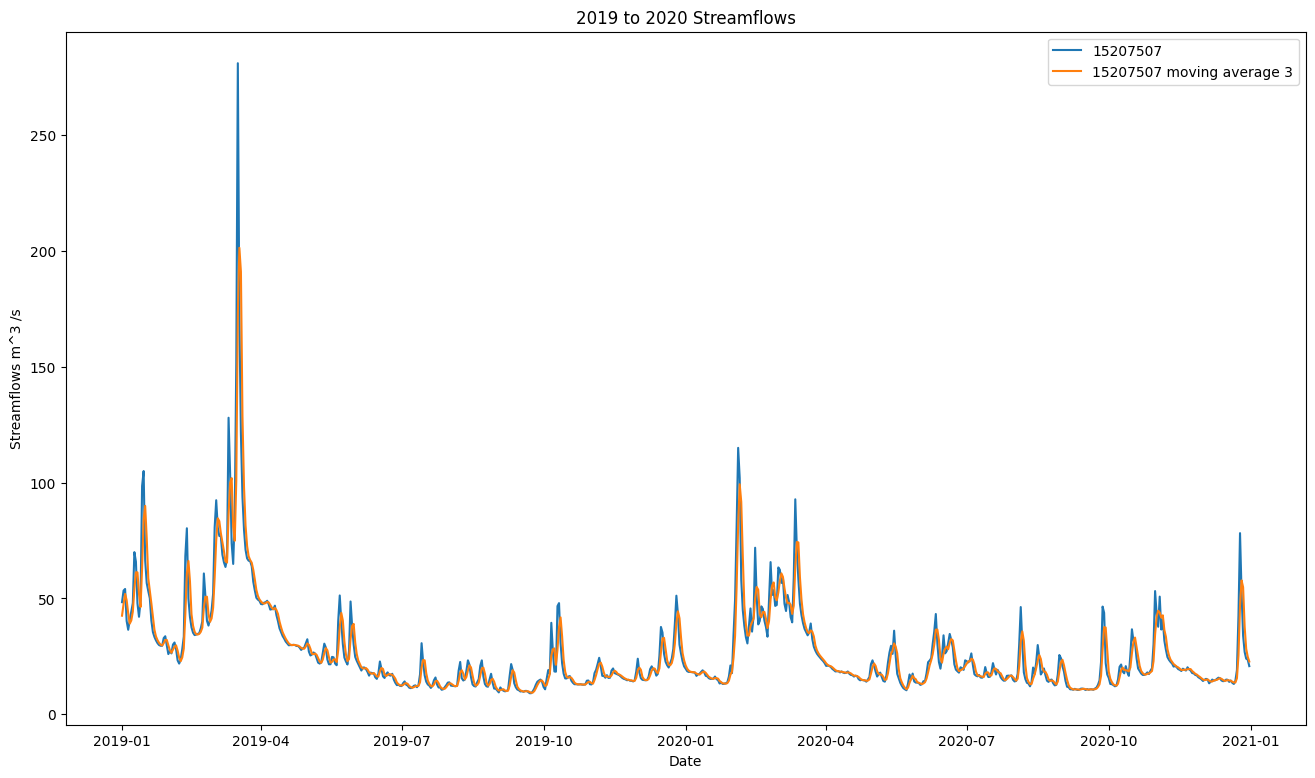
\includegraphics[width=0.8\linewidth]{work/07-hydroLSTM/images/Moving_Average} 

}

\caption{streamflows of the 15207507 Marienthal gauging stations before (blue) and after (orange) applying moving average smoothing}\label{fig:marien-stream}
\end{figure}

To combine the rasterized meteorological data from ERA5 with the streamflows of the Regen, it is necessary to only take precipitation into account that occurs within the defined catchments. To achieve this, a weighted average is calculated, where the weights are determined by the area size of the intersection between the raster cell of the meteorological data and the catchment. This can be seen in a schematic visualization in figure \ref{fig:spatial-avg}.

\begin{figure}

{\centering 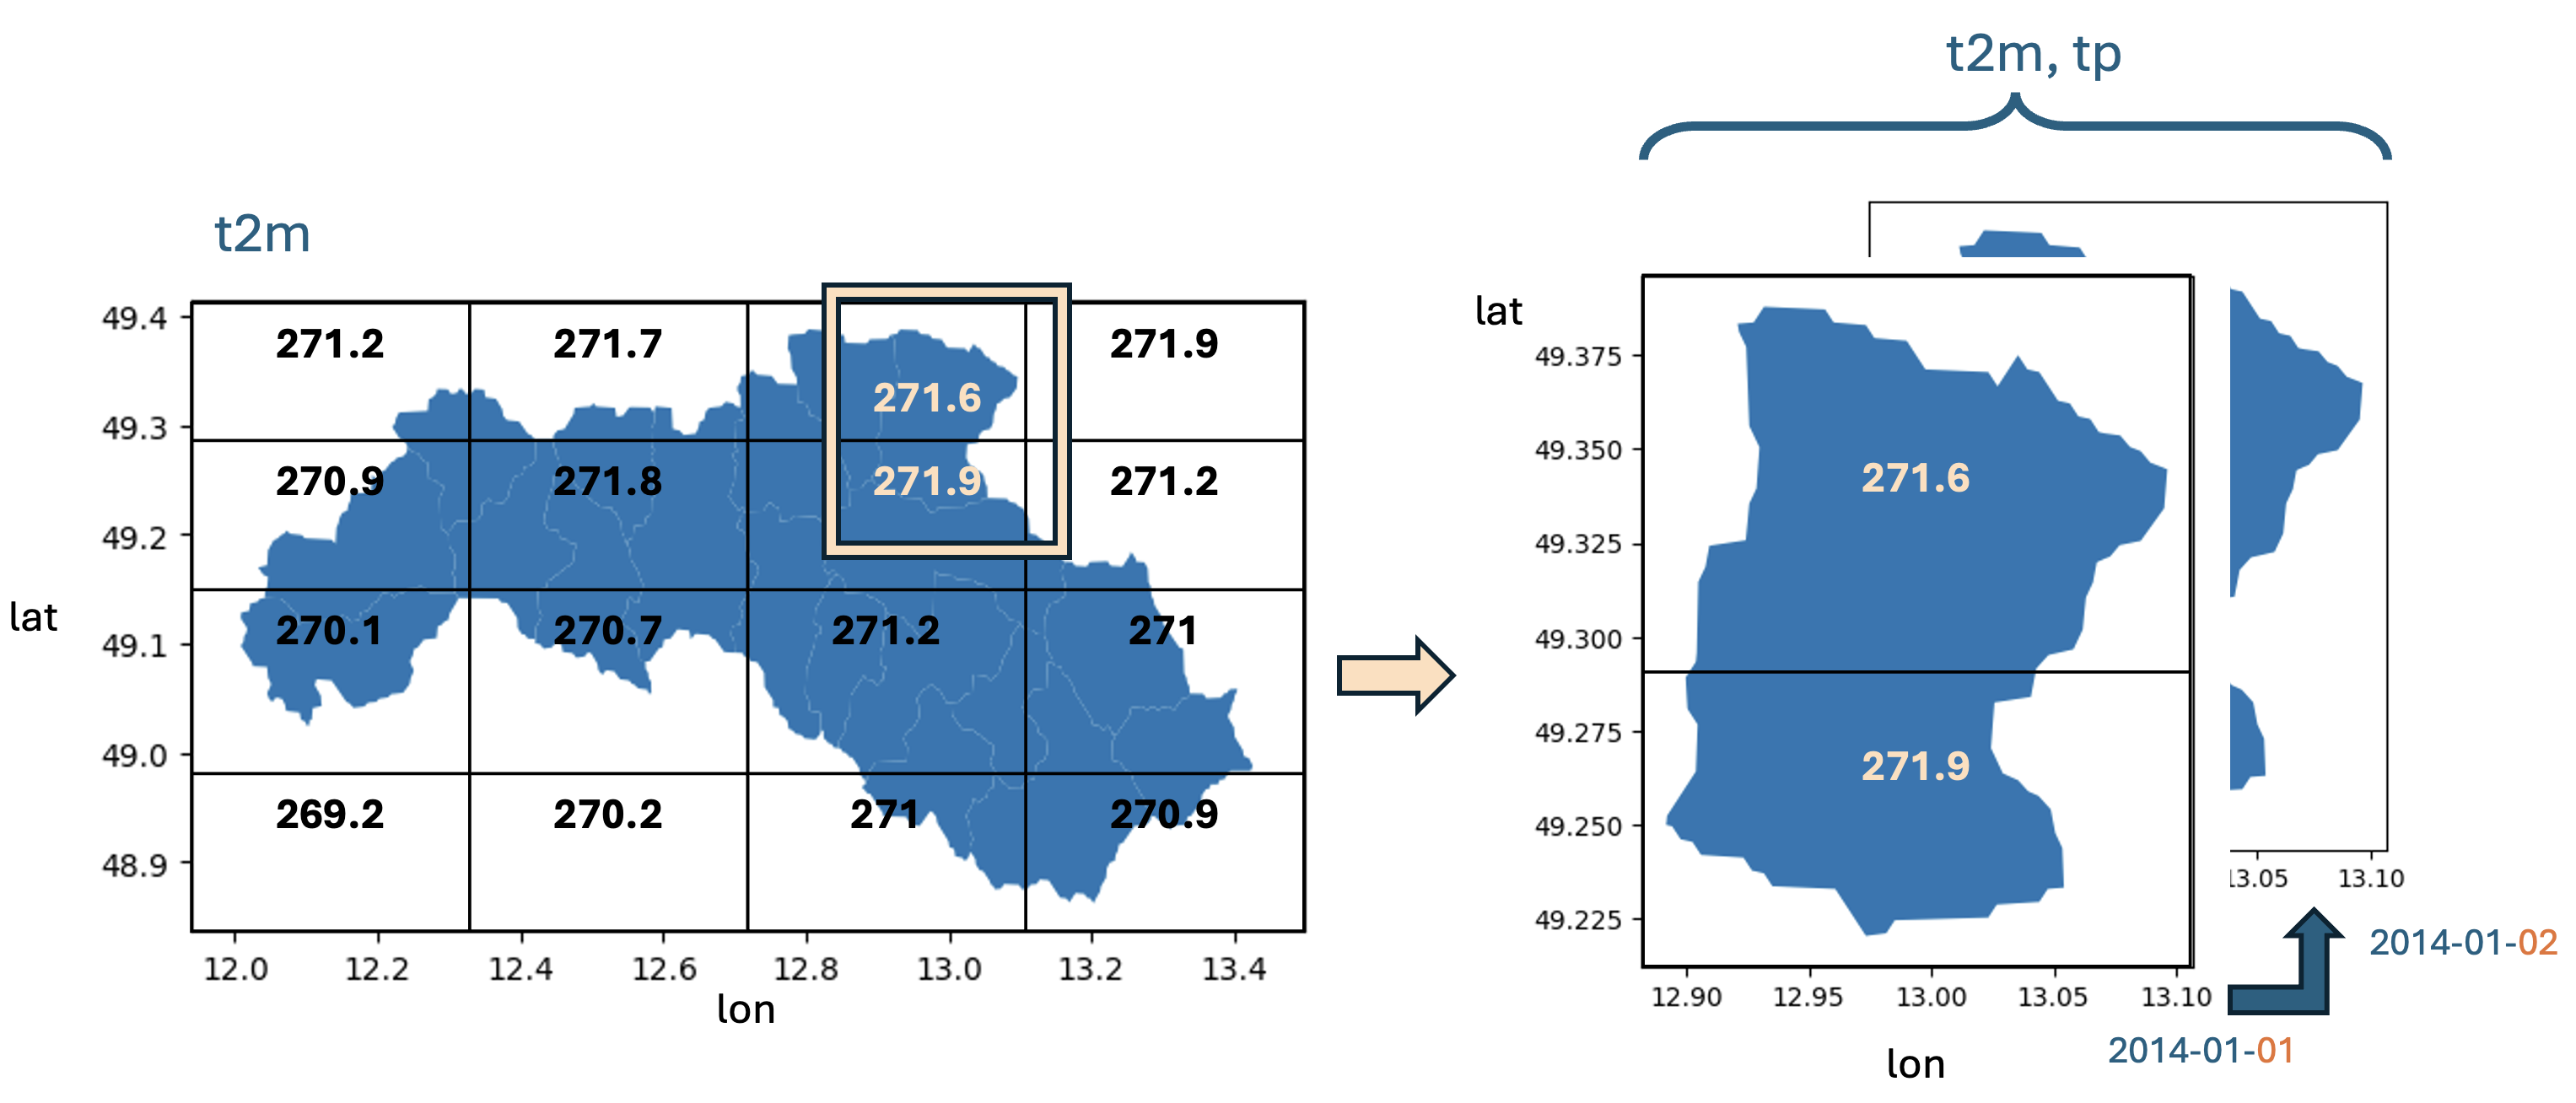
\includegraphics[width=0.8\linewidth]{work/07-hydroLSTM/images/spatial_averaging} 

}

\caption{schematic visualization of the spatial averaging performed for temperature and total precipitation during data preprocessing}\label{fig:spatial-avg}
\end{figure}

\[ tp(\text{catch}_i) = \frac{1}{A(\text{catch}_i)} \sum_{cell_j \in \text{ERA5 raster}} \left( tp(\text{cell}_j) \cdot A(\text{catch}_i \cap \text{cell}_j) \right) \tag{1} \]

A : area\\
catch : catchment\\
cell : one cell in the raster data set of ERA5\\
tp : total precipitation

Since the catchments are geospatially very close to each other, the different catchments are highly correlated to each other and therefore provide little variance (see Figure \ref{fig:tp-corr}). To reduce the feature space for both variables temperature and precipitation, the mean is taken over all catchments. Finally to reduce the noise in the features a moving average of window size 3 was applied.

\begin{figure}

{\centering 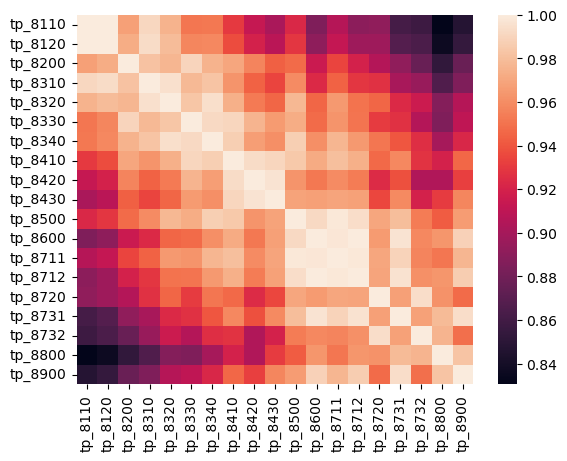
\includegraphics[width=0.7\linewidth]{work/07-hydroLSTM/images/tp_correlation_table} 

}

\caption{correlation table for total precipitation over all catchments}\label{fig:tp-corr}
\end{figure}

\section{Models}\label{models}

\subsection{LSTM}\label{lstm}

The Long Short-Term Memory (LSTM) cell (figure \ref{fig:lstm}) is a type of recurrent neural network (RNN) architecture designed to model temporal sequences and their long-range dependencies more accurately than traditional RNNs. LSTMs were introduced by Sepp Hochreiter and Jürgen Schmidhuber in 1997 to address the issue of vanishing and exploding gradients encountered in traditional RNNs \citet{hochreiter}.

\begin{figure}

{\centering 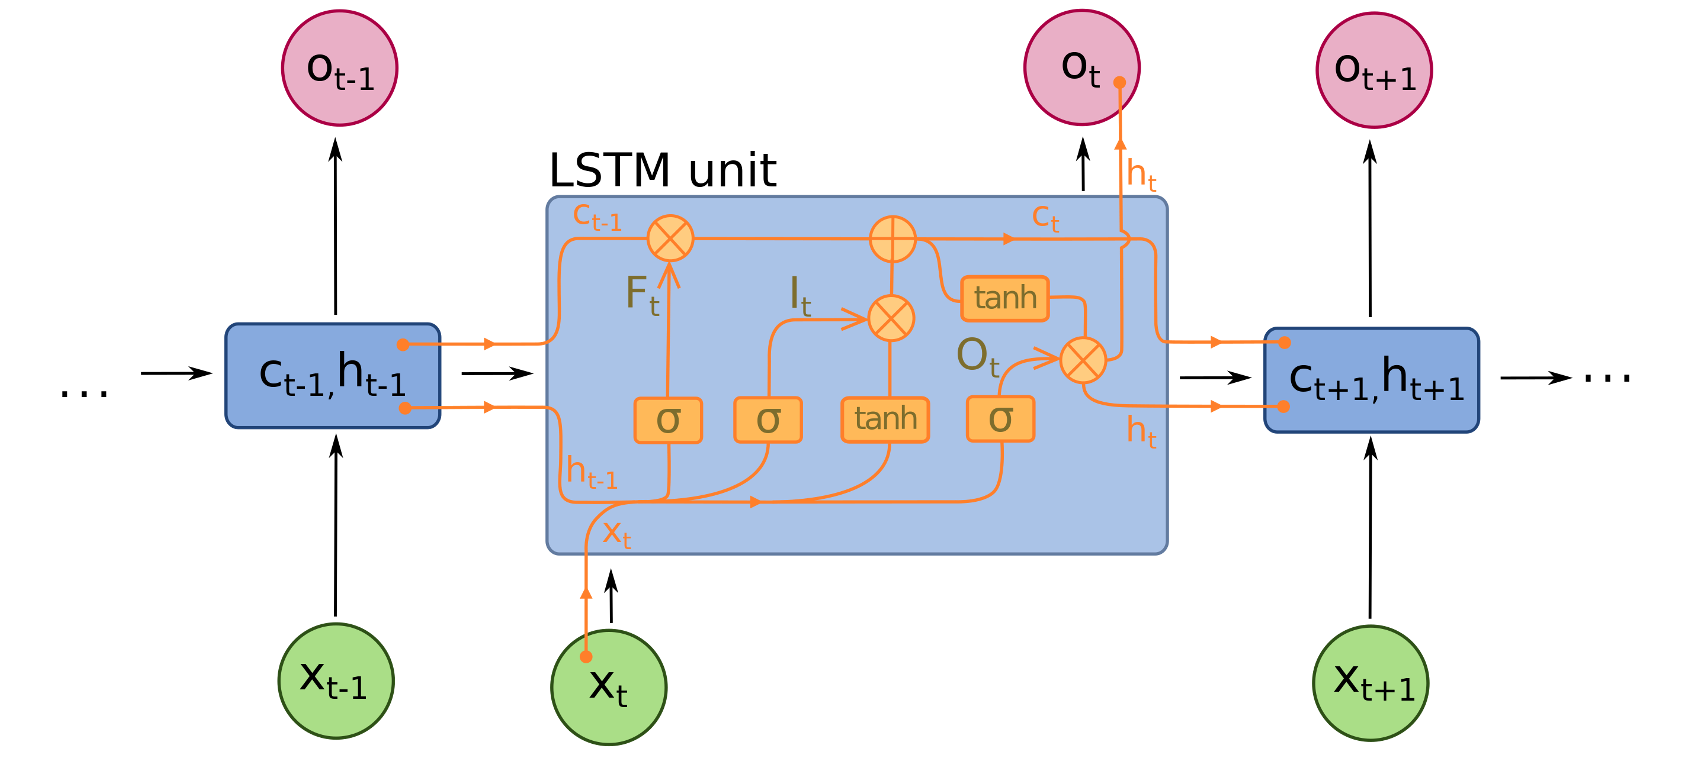
\includegraphics[width=0.7\linewidth]{work/07-hydroLSTM/images/LSTM} 

}

\caption{visualization of a LSTM cell at time step t (image adapted from @lstmimage)}\label{fig:lstm}
\end{figure}

\begin{enumerate}
\def\labelenumi{\arabic{enumi}.}
\tightlist
\item
  \textbf{Cell State (}\(C_t\)): The internal memory of the cell, which can carry information across many time steps.
\item
  \textbf{Hidden State (}\(h_t\)): The output of the LSTM cell at a given time step, also serving as the input to the next cell.
\item
  \textbf{Input Gate (}\(i_t\)): Controls how much of the new information from the current input is used to update the cell state.
\item
  \textbf{Forget Gate (}\(f_t\)): Decides how much of the past cell state should be forgotten.
\item
  \textbf{Output Gate (}\(o_t\)): Determines the output of the LSTM cell based on the cell state.
\end{enumerate}

LSTMs are particularly well-suited for tasks that involve sequential data and temporal dependencies, such as:

\begin{enumerate}
\def\labelenumi{\arabic{enumi}.}
\tightlist
\item
  \textbf{Natural Language Processing (NLP)}:

  \begin{itemize}
  \tightlist
  \item
    Language modeling
  \item
    Machine translation
  \item
    Speech recognition
  \end{itemize}
\item
  \textbf{Time Series Forecasting}:

  \begin{itemize}
  \tightlist
  \item
    Stock price prediction
  \item
    Weather forecasting
  \item
    Anomaly detection
  \end{itemize}
\end{enumerate}

Streamflow forecasting involves predicting the flow of water in rivers and streams over time, which is inherently a time-series problem with temporal dependencies influenced by various factors such as rainfall, snowmelt, and upstream water management. When used in an encoder decoder architecture LSTM-cells can also incorporate future known covariates such as weather forecasts. These specifications make LSTM-based architectures beneficial for modeling and forecasting streamflow data.

\subsection{Temporal Fusion Transformer}\label{temporal-fusion-transformer}

The Temporal Fusion Transformer (TFT) (figure \ref{fig:tft}) is a neural network architecture specifically designed for multi-horizon time series forecasting. It combines the strengths of both recurrent and attention-based models, offering an advanced approach to handling complex time series data. The TFT was introduced by Bryan Lim et al.~in 2019, aiming to provide interpretability and accuracy for forecasting tasks \citet{LIM20211748}.

\begin{figure}

{\centering 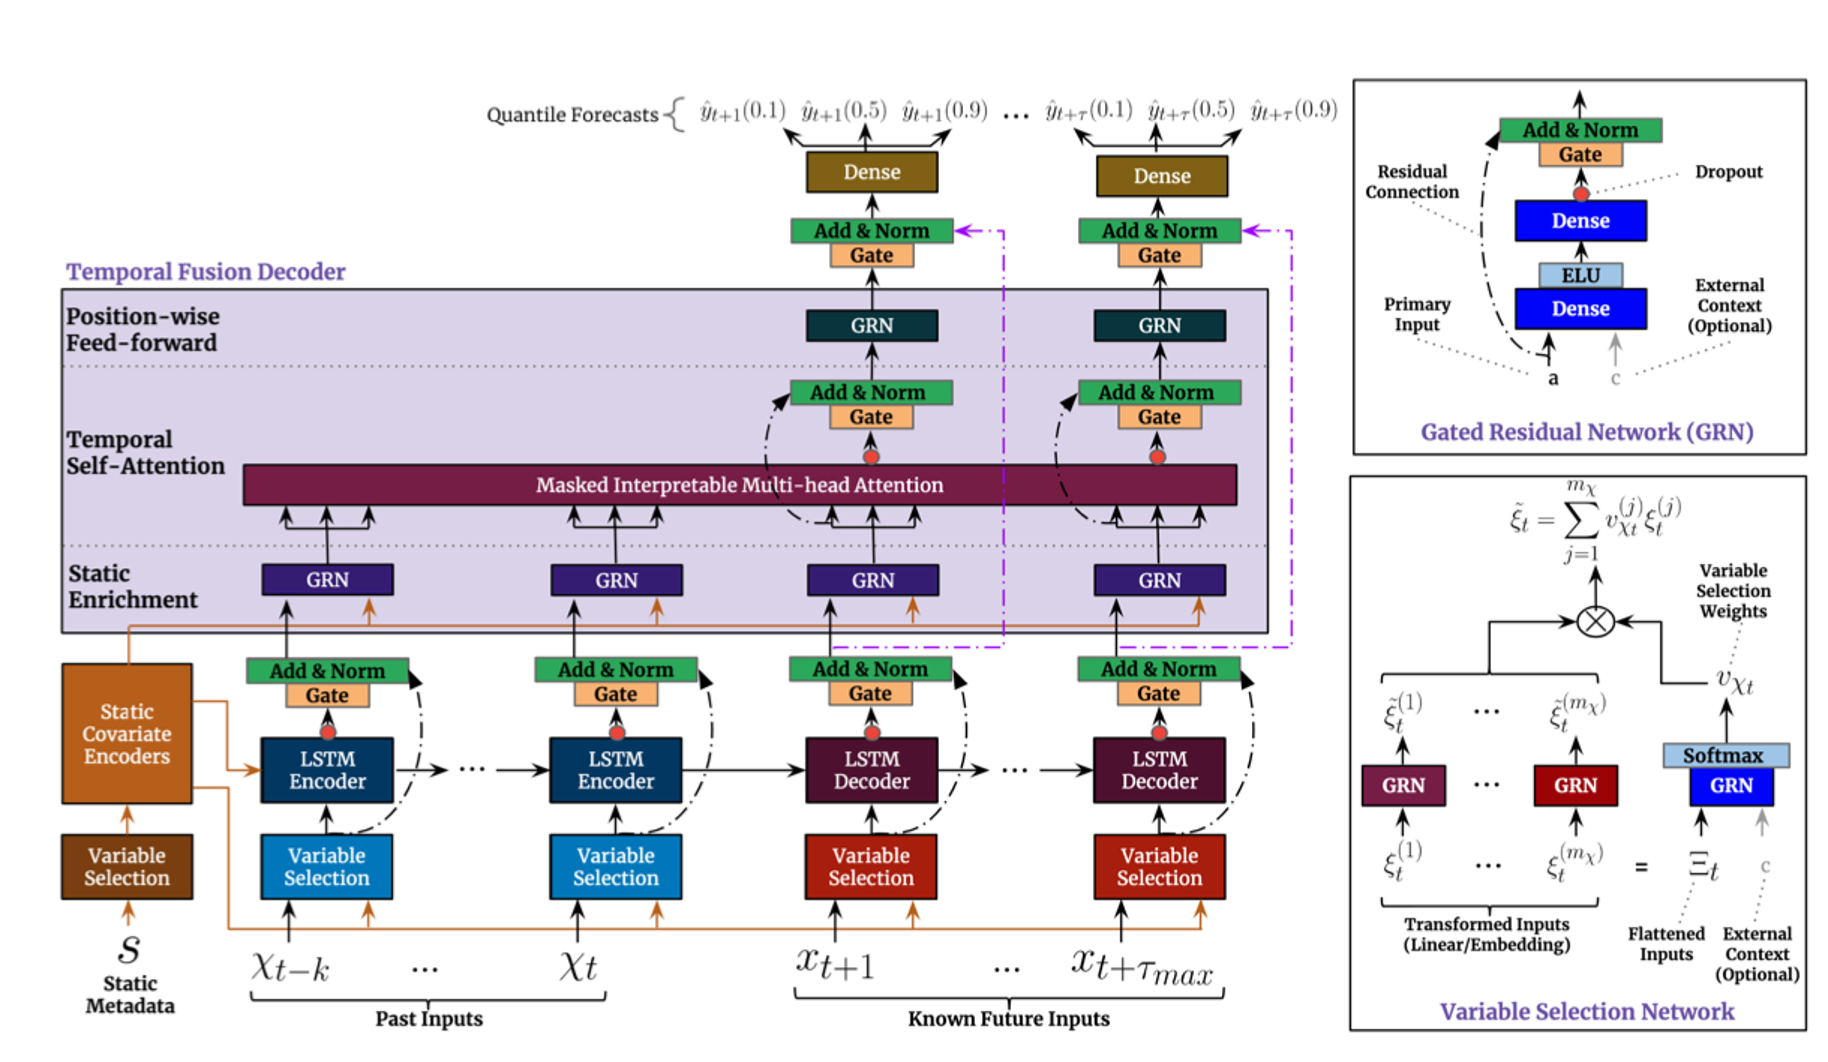
\includegraphics[width=0.8\linewidth]{work/07-hydroLSTM/images/TFT} 

}

\caption{model architecture for the Temporal Fusion Transformer (image from @LIM20211748}\label{fig:tft}
\end{figure}

A TFT consists of several key components:

\begin{enumerate}
\def\labelenumi{\arabic{enumi}.}
\tightlist
\item
  \textbf{Temporal Processing}:

  \begin{itemize}
  \tightlist
  \item
    \textbf{Local Processing with LSTMs}: LSTMs are used to process local temporal dependencies within the time series.
  \item
    \textbf{Multi-Head Attention}: An attention mechanism to capture long-range dependencies across different time steps.
  \end{itemize}
\item
  \textbf{Variable Selection}:

  \begin{itemize}
  \tightlist
  \item
    \textbf{Static Covariate Encoders}: Handle static features that do not change over time (e.g., location-specific data).
  \item
    \textbf{Temporal Covariate Encoders}: Manage time-varying features (e.g., weather data, past values of the time series).
  \end{itemize}
\item
  \textbf{Gating Mechanisms}:

  \begin{itemize}
  \tightlist
  \item
    \textbf{Gated Residual Network (GRN)}: Ensures that only relevant information is passed through layers, improving the network's efficiency and interpretability.
  \item
    \textbf{Variable Selection Networks}: Dynamically select relevant variables at each time step to enhance model performance and interpretability.
  \end{itemize}
\item
  \textbf{Multi-Horizon Forecasting}:

  \begin{itemize}
  \tightlist
  \item
    \textbf{Sequence-to-Sequence Framework}: Allows the TFT to generate forecasts for multiple future time steps simultaneously.
  \end{itemize}
\item
  \textbf{Interpretable Outputs}:

  \begin{itemize}
  \tightlist
  \item
    \textbf{Attention Weights}: Provide insights into which time steps and variables the model is focusing on, aiding interpretability.
  \end{itemize}
\end{enumerate}

The Temporal Fusion Transformer represents an advancement in time series forecasting, offering both high accuracy and interpretability. Its ability to capture complex dependencies, dynamically select relevant features, and provide insights into the decision-making process makes it a useful tool for streamflow forecasting.

\subsection{Kling Gupta Efficiency}\label{kling-gupta-efficiency}

The Kling-Gupta Efficiency (KGE) is a statistical metric used to evaluate the performance of hydrological models by comparing simulated data to observed data. Developed by Gupta et al.~in 2009, the KGE addresses limitations found in traditional metrics such as the Nash-Sutcliffe Efficiency (NSE). The KGE decomposes the evaluation of model performance into three distinct components, providing a more comprehensive assessment. These components are correlation, bias, and variability, which help in understanding different aspects of the model's accuracy.

The KGE is calculated using the following formula:

\[ \text{KGE} = 1 - \sqrt{(r - 1)^2 + (\alpha - 1)^2 + (\beta - 1)^2} \tag{2} \]

\begin{itemize}
\item
  \(r\) is the Pearson correlation coefficient between the simulated and observed values.
\item
  \(\alpha\) is the bias ratio, defined as the ratio of the mean of the simulated values to the mean of the observed values.
\item
  \(\beta\) is the standard deviation ratio, defined as the ratio of the standard deviation of the simulated values to the standard deviation of the observed values.
\end{itemize}

\section{Results}\label{results}

\subsection{Training Setup}\label{training-setup}

The 2 different model architectures were trained using the historical streamflows as well as temperature and precipitation as covariates. Using an input sequence length of 364 days and an output lead time of up to 7 days. Temperature and precipitation can be used as future known values when considering weather forecasts. For example when trying to predict one step ahead forecast for the streamflow in addition to the past 364 days of precipitation values one can consider the precipitation forecast for the next day to get the best predictions possible.

The LSTM Model is run in an encoder decoder architecture, were the past 364 days are the input for an LSTM cell which returns a hidden state and an output as the encoder step. During the decoder step, the encoder hidden state is fed into the decoder LSTM together with the future known inputs. The model predicts incrementally in the sense that for example to predict a 3 step ahead forecast it firsts predicts 1 and 2 step forecast and uses both forecasts to then predict the 3 step prediction. Both model architectures were used from the pytorch-forecasting library. The models were retrained for the different lead times. The used hyperparameters for both models are shown in Table \ref{tab:tab-hyperparams}.

The dataset is split into 70\% train set, 15\% validation set and 15\% test set respectivell.

\begin{table}

\caption{\label{tab:tab-hyperparams}Hyperparameter comparison between LSTM and TFT.}
\centering
\begin{tabular}[t]{l|l|l}
\hline
Hyperparameter & LSTM & TFT\\
\hline
Batch Size & 128 & 128\\
\hline
Epochs & 100 & 80\\
\hline
Hidden Size & 128 & 128\\
\hline
Attention Head Size & - & 2\\
\hline
Learning Rate & 0.001 & 0.003\\
\hline
Dropout & 0.2 & 0.1\\
\hline
Weight Decay & 0.001 & 1e-04\\
\hline
Gradient Clipping & 0.1 & 0.1\\
\hline
Loss Function & Mean Absolute Error & Mean Absolute Error\\
\hline
Optimizer & Adam & Adam\\
\hline
Reduce on Plateau Patience & 7 & 7\\
\hline
Time Varying Known Features & t2m, tp & t2m, tp\\
\hline
Time Varying Unknown Features & streamflow 15207507 & streamflow 15207507\\
\hline
\end{tabular}
\end{table}

\subsection{Results}\label{results-1}

The models evaluated on the holdout test set show good performance for lead times of 1 and 2 days especially considering since the training and validation loss that is used is the MAE and not the KGE. The performance declines sharply for the LSTM model across the lead times while the decline for the TFT is more gradual as can be seen in Table \ref{tab:tab-results}.

\begin{longtable}[]{@{}rll@{}}
\caption{\label{tab:tab-results}Performance comparison between TFT and LSTM models across different lead times on a holdout test set. Better performing model for each lead time in bold}\tabularnewline
\toprule\noalign{}
Lead.Time & TFT.KGE & LSTM.KGE \\
\midrule\noalign{}
\endfirsthead
\toprule\noalign{}
Lead.Time & TFT.KGE & LSTM.KGE \\
\midrule\noalign{}
\endhead
\bottomrule\noalign{}
\endlastfoot
1 & 0.8352 & \textbf{0.9696} \\
2 & 0.7103 & \textbf{0.8821} \\
3 & 0.6410 & \textbf{0.6716} \\
4 & \textbf{0.6096} & 0.4943 \\
5 & \textbf{0.5901} & 0.4302 \\
6 & \textbf{0.5778} & 0.3312 \\
7 & \textbf{0.5717} & 0.3185 \\
\end{longtable}

Forecasting the peaks of the streamflows is challenging and neither model performs particularly well on this task. Especially when considering that the peaks were already drastically reduced due to the moving average smoothing of the target variable. The model routinely undershoots the observed true streamflows here shown for a lead time of 5 days for the LSTM Model and the TFT Model in figure \ref{fig:lstm-pred} and in figure \ref{fig:tft-pred} respectively. This behavior can be observed for all lead times except 1 and 2 days where the performance is reasonable even in the peaks.

\begin{figure}

{\centering 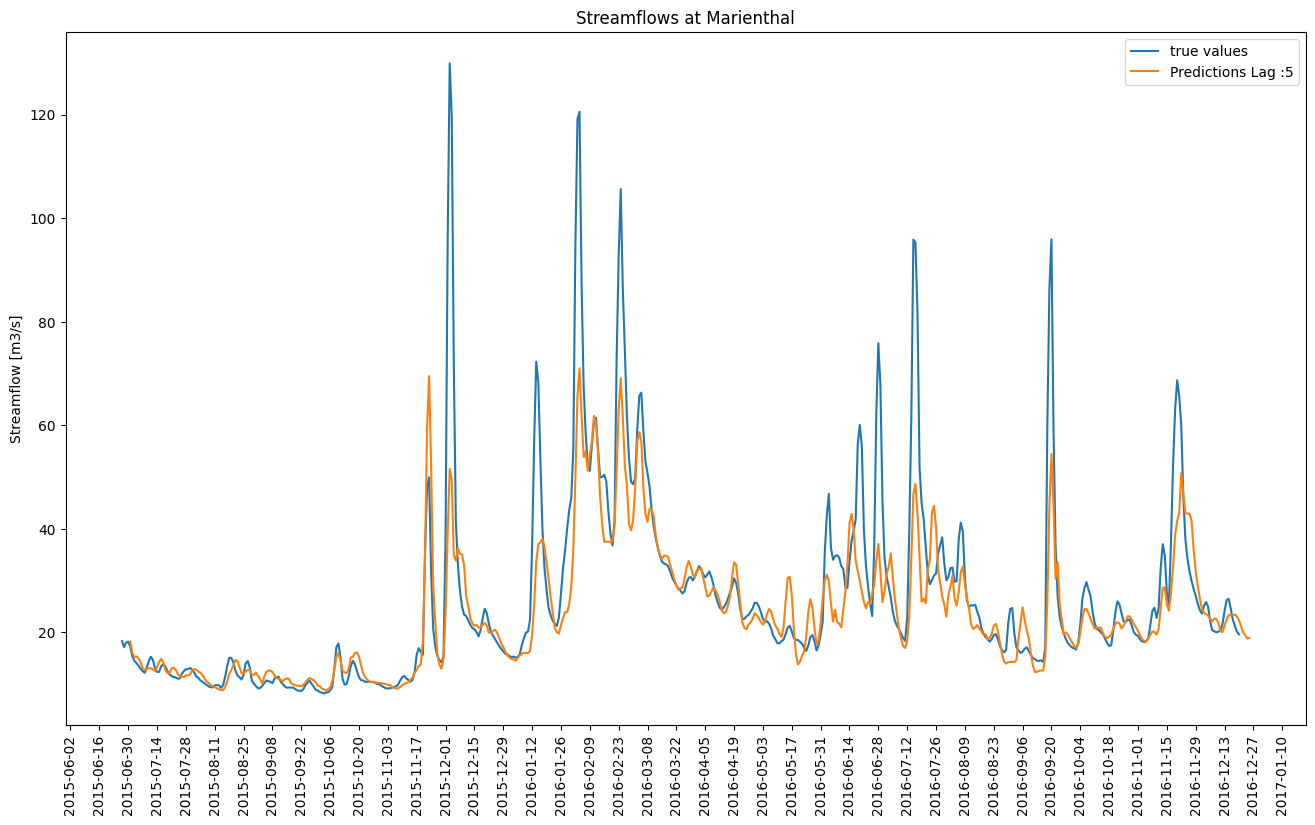
\includegraphics[width=0.8\linewidth]{work/07-hydroLSTM/images/lag5_lstm} 

}

\caption{LSTM predicted streamflows for a lead time of 5 days (orange) compared to the observed streamflows (blue)}\label{fig:lstm-pred}
\end{figure}

\begin{figure}

{\centering 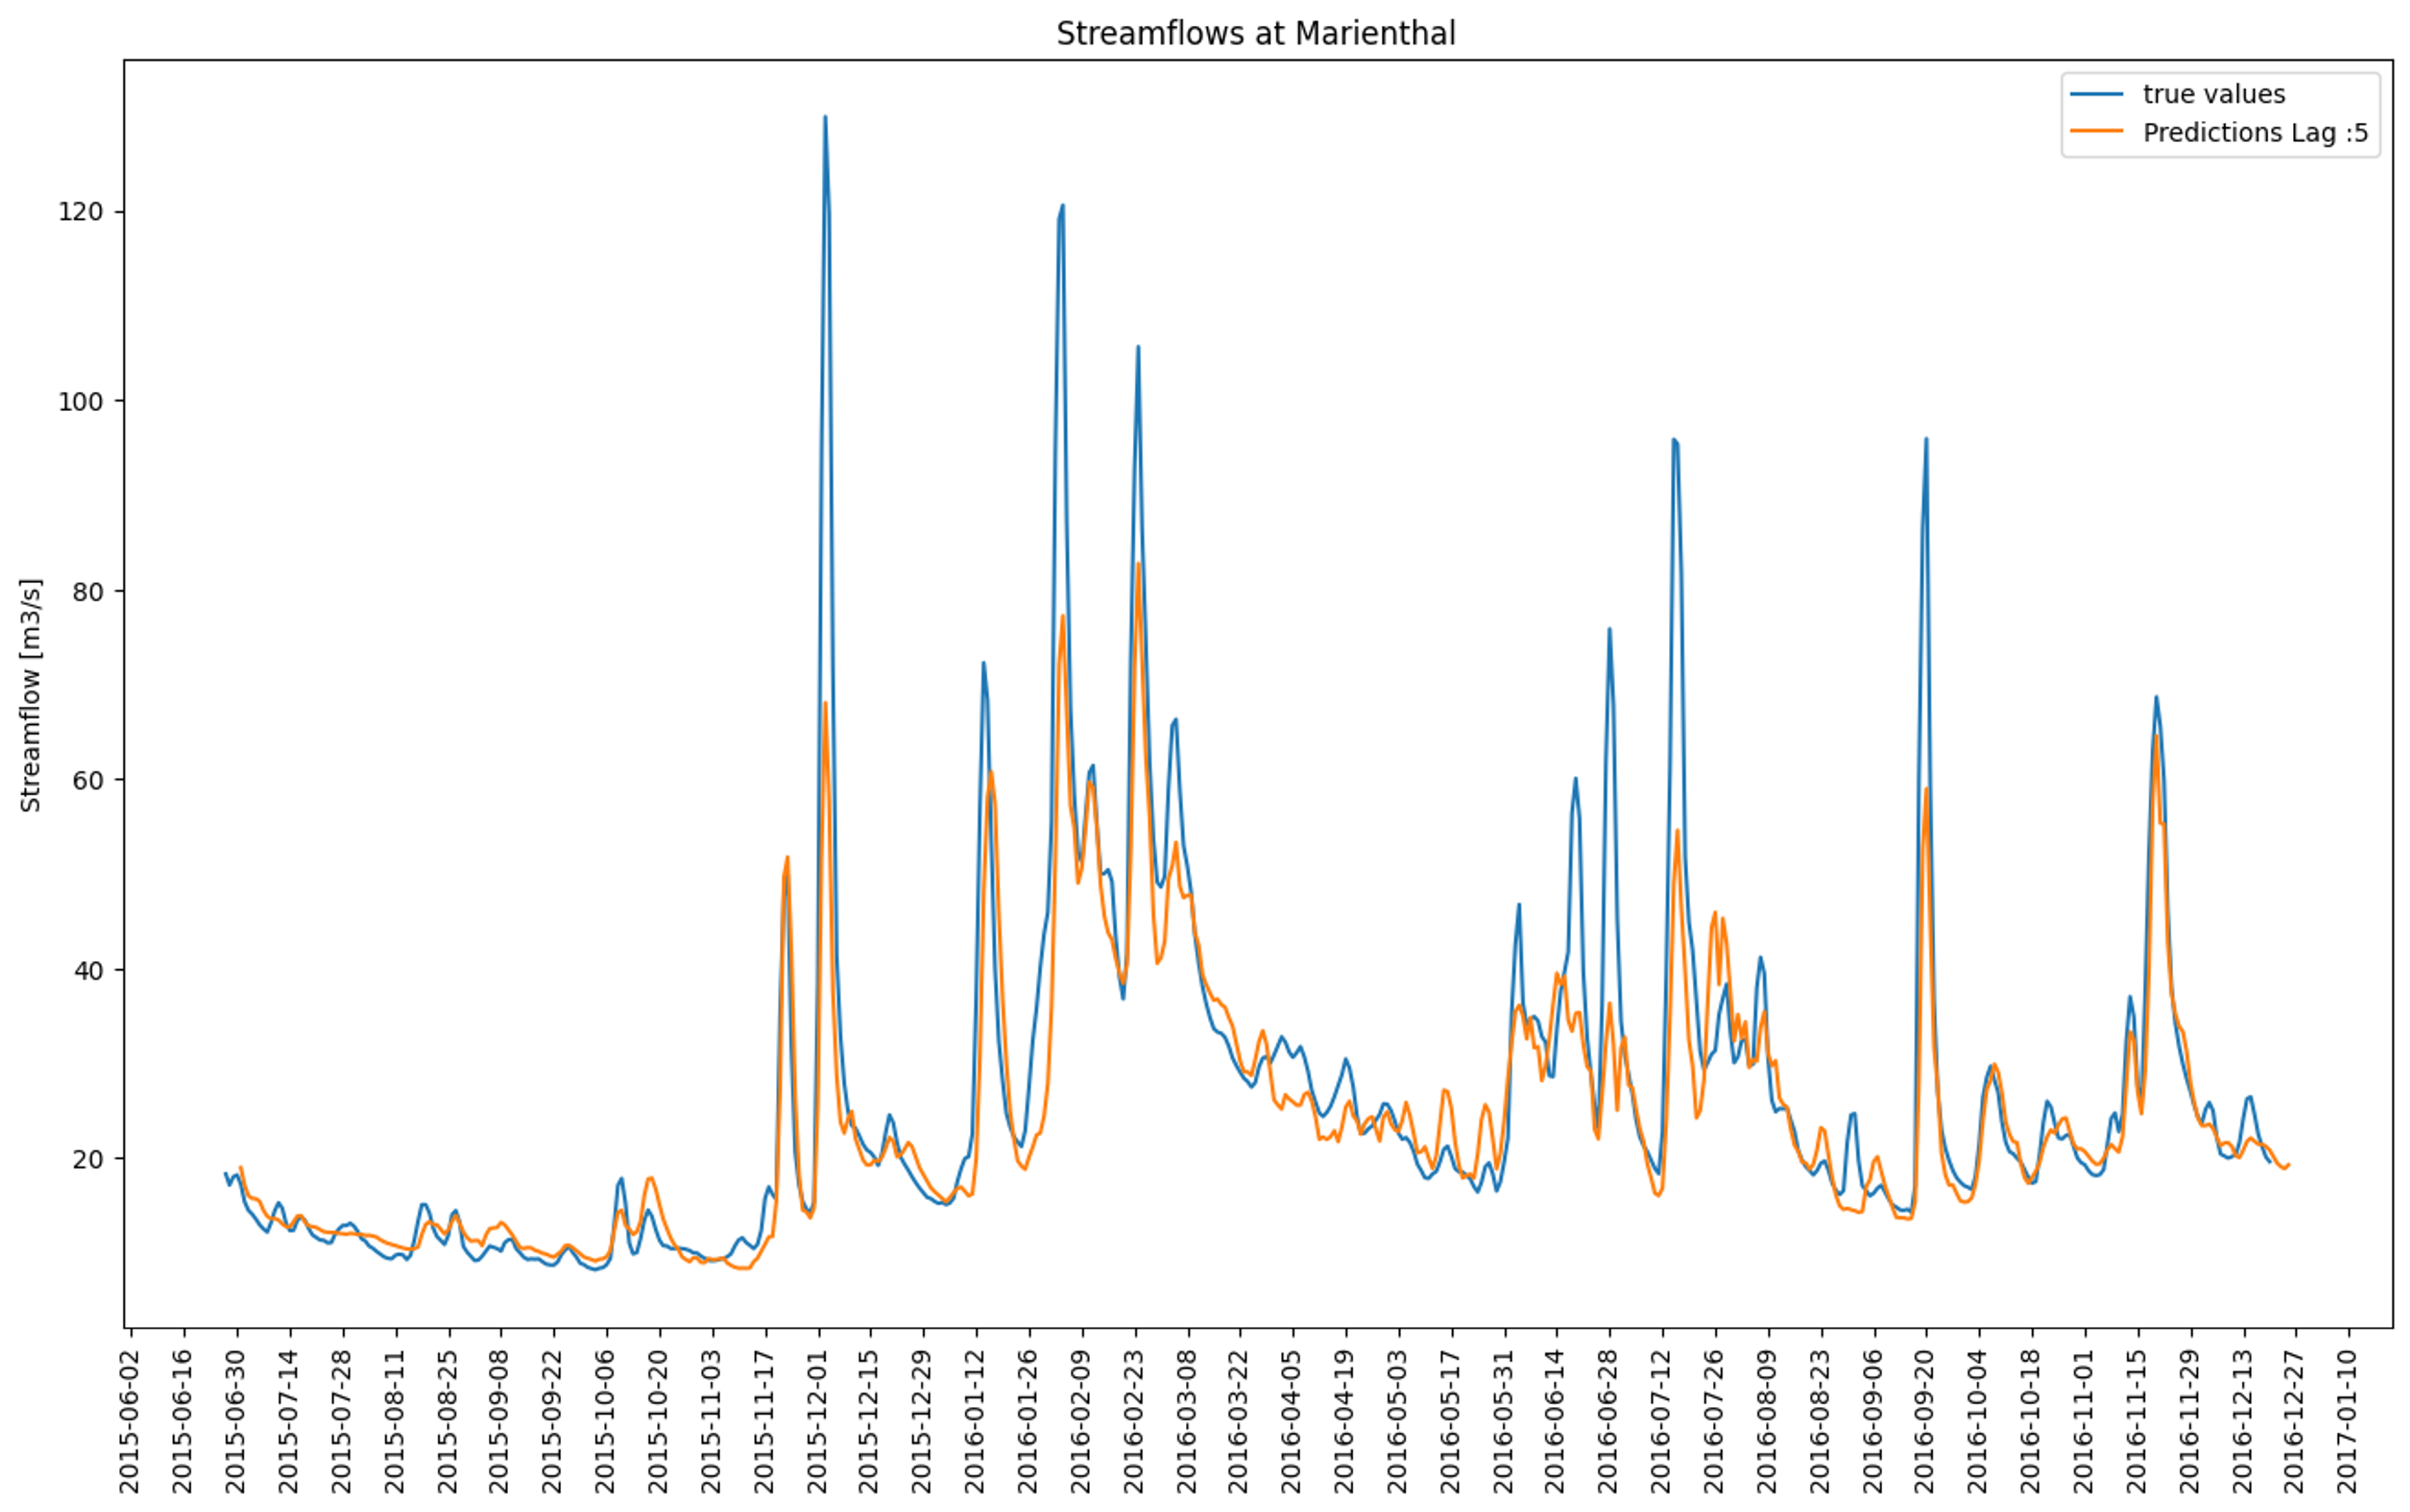
\includegraphics[width=0.8\linewidth]{work/07-hydroLSTM/images/lag5_tft} 

}

\caption{TFT predicted streamflows for a lead time of 5 days (orange) compared to the observed streamflows (blue)}\label{fig:tft-pred}
\end{figure}

\subsection{Feature Importance}\label{feature-importance}

For an inspection of feature dependence it is possible to make use of the inbuilt function that the pytorch-forecasting library provides. The models show very similar behavior for both used covariates. As can be seen in \ref{fig:tp-tft-imp} the TFT model observes a slightly stronger relationship between high total precipitation and large streamflows, but the plot for for both models has the expected shape, that high precipitation leads to high streamflows and vice versa.

In analyzing the relationship between t2m and streamflow, both graphs demonstrate a positive relationship. Specifically, the TFT dependence plot in Figure \ref{fig:t2m-tft-imp} shows an increase up to approximately 280 K, beyond which the effect plateaus. Similarly, the LSTM model depicted in Figure \ref{fig:t2m-lstm-imp} shows a more gradual increase, with the effect leveling off at higher mean temperatures of around 295 K.

\begin{figure}

{\centering 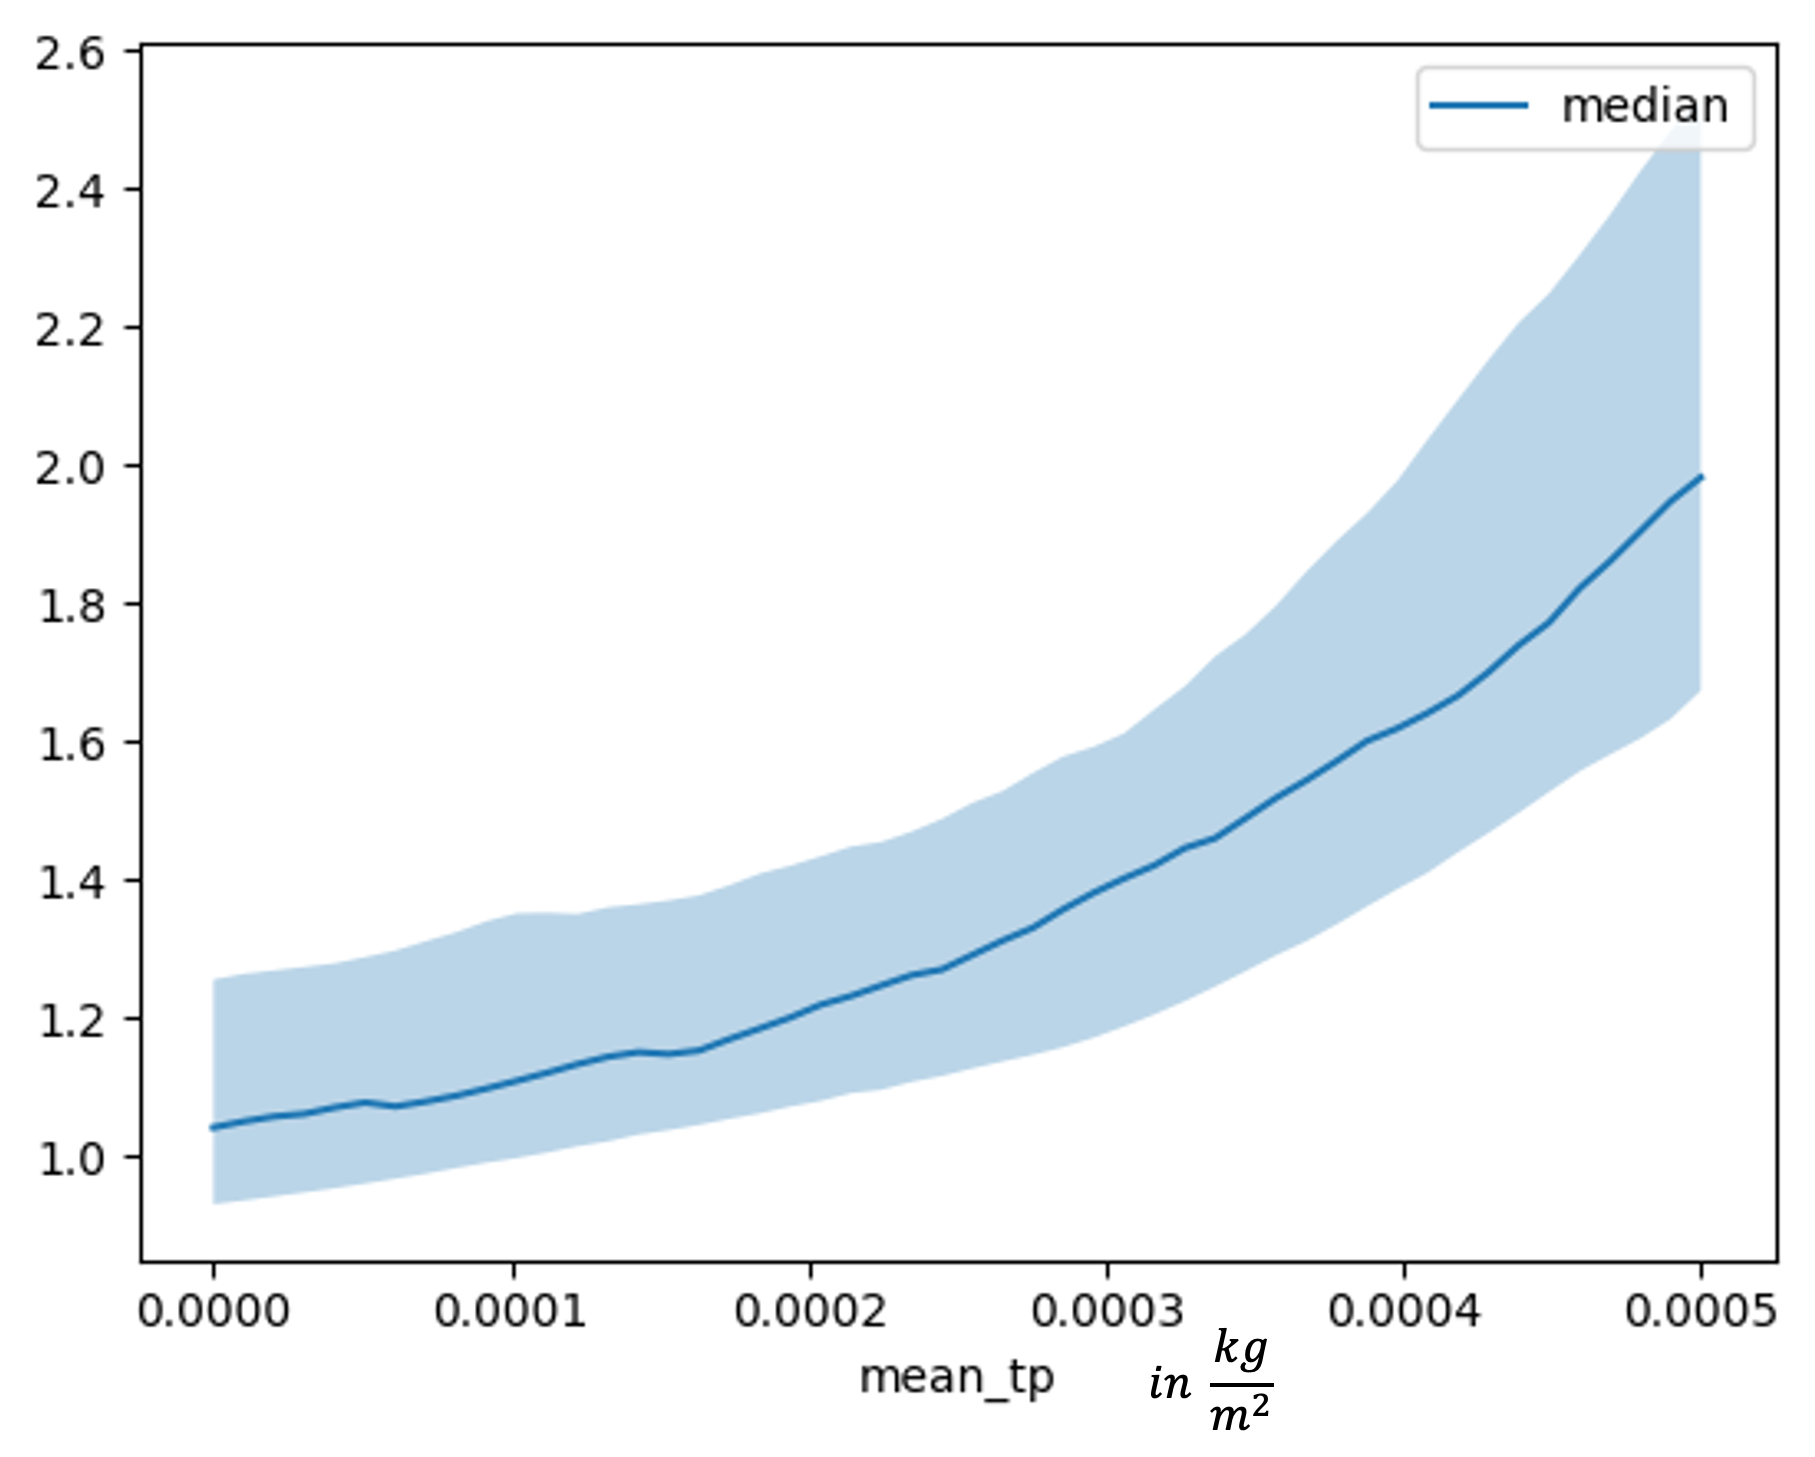
\includegraphics[width=0.7\linewidth]{work/07-hydroLSTM/images/mean_tp_feature_importance_lstm} 

}

\caption{Feature dependence plot for mean total precipitation for a lead time 5 trained LSTM}\label{fig:tp-lstm-imp}
\end{figure}

\begin{figure}

{\centering 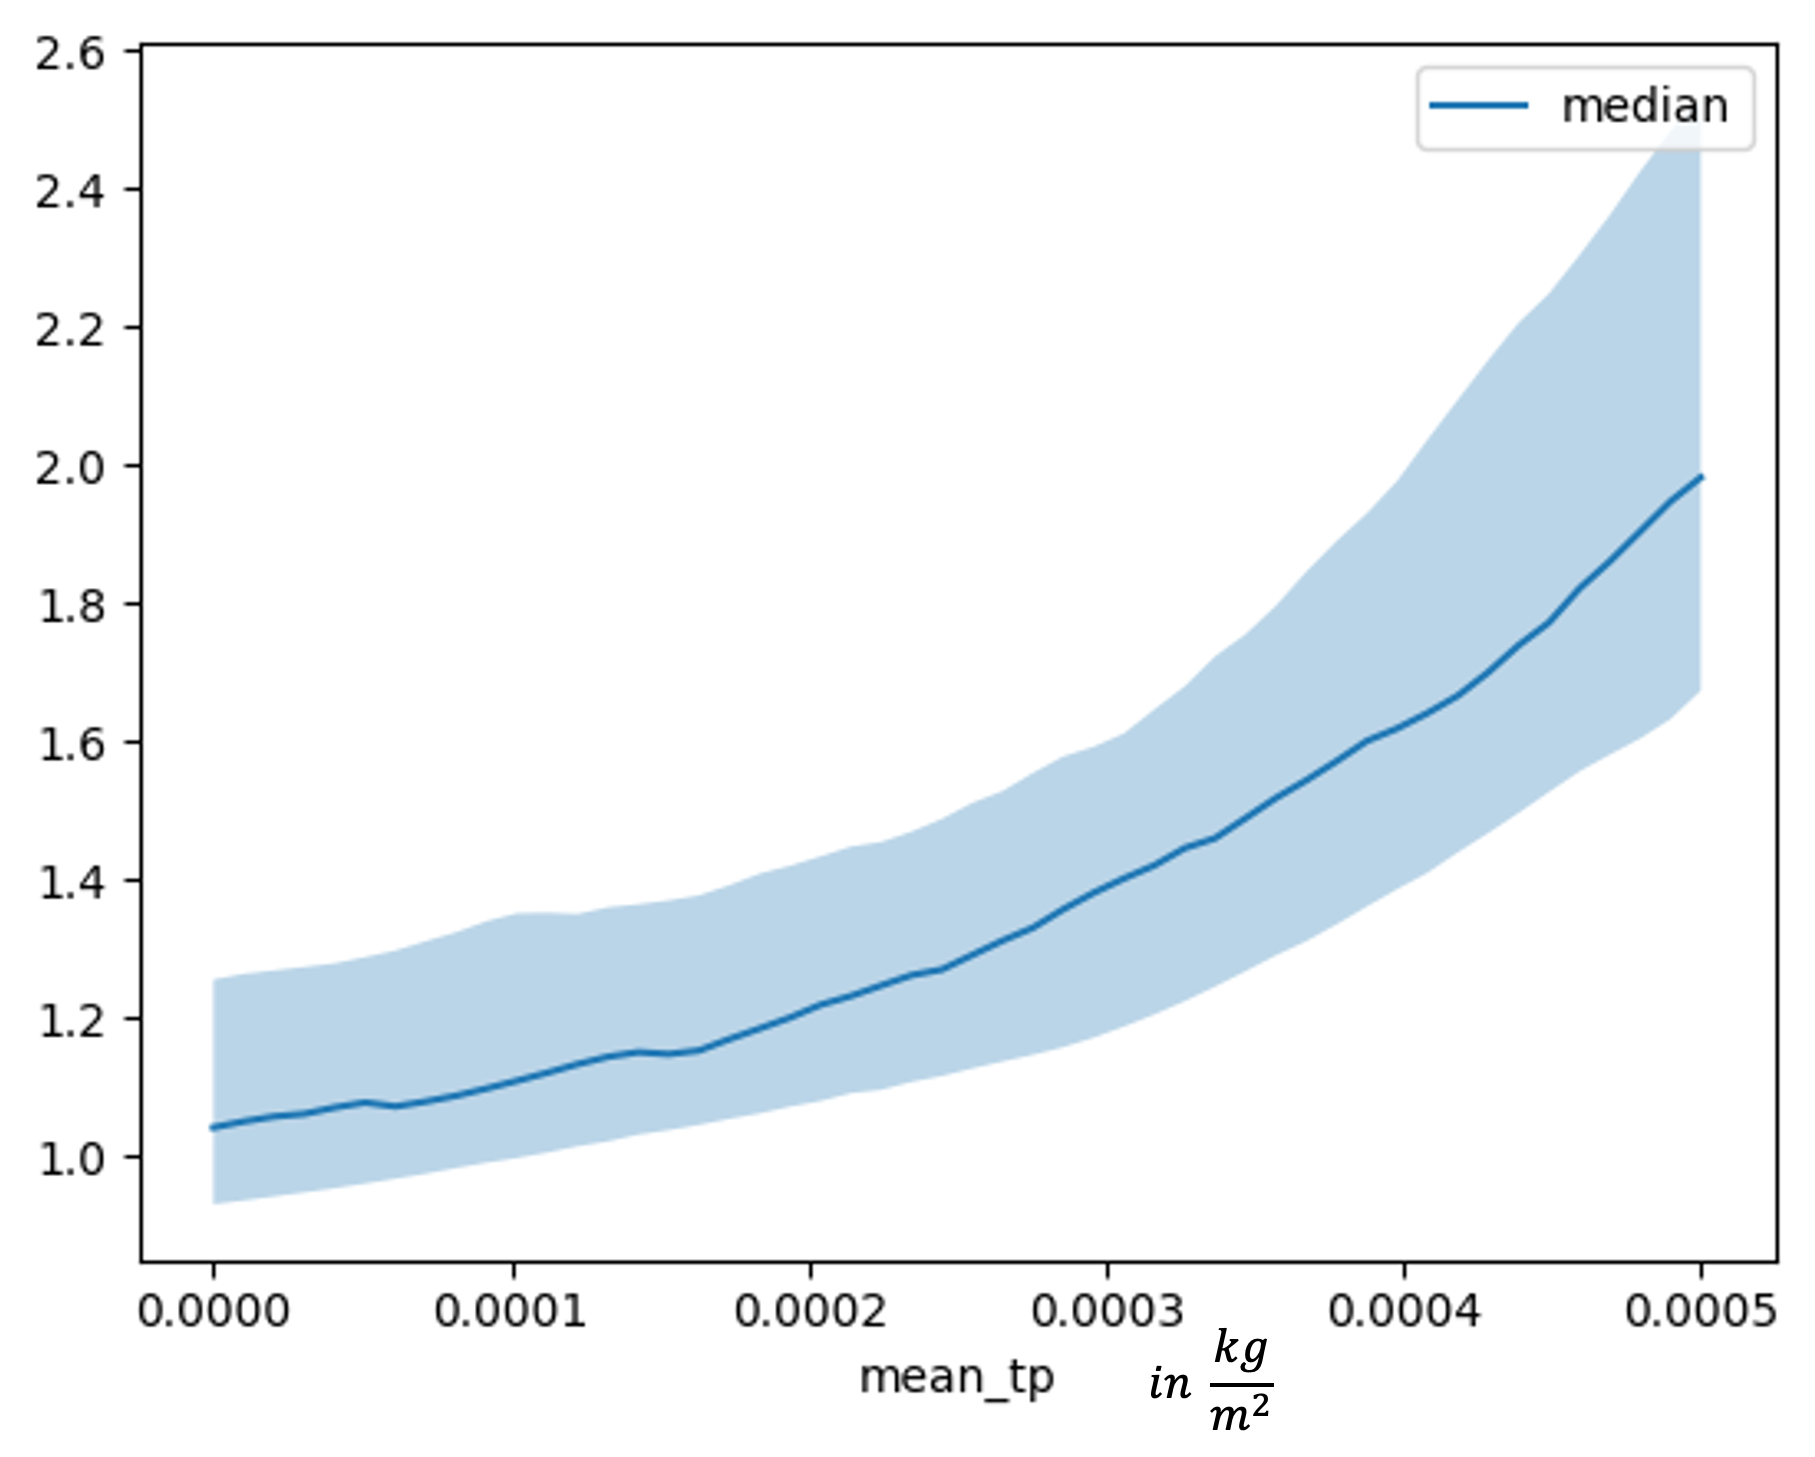
\includegraphics[width=0.7\linewidth]{work/07-hydroLSTM/images/mean_tp_feature_importance_tft} 

}

\caption{Feature dependence plot for mean total precipitation for a lead time 5 trained TFT}\label{fig:tp-tft-imp}
\end{figure}

\begin{figure}

{\centering 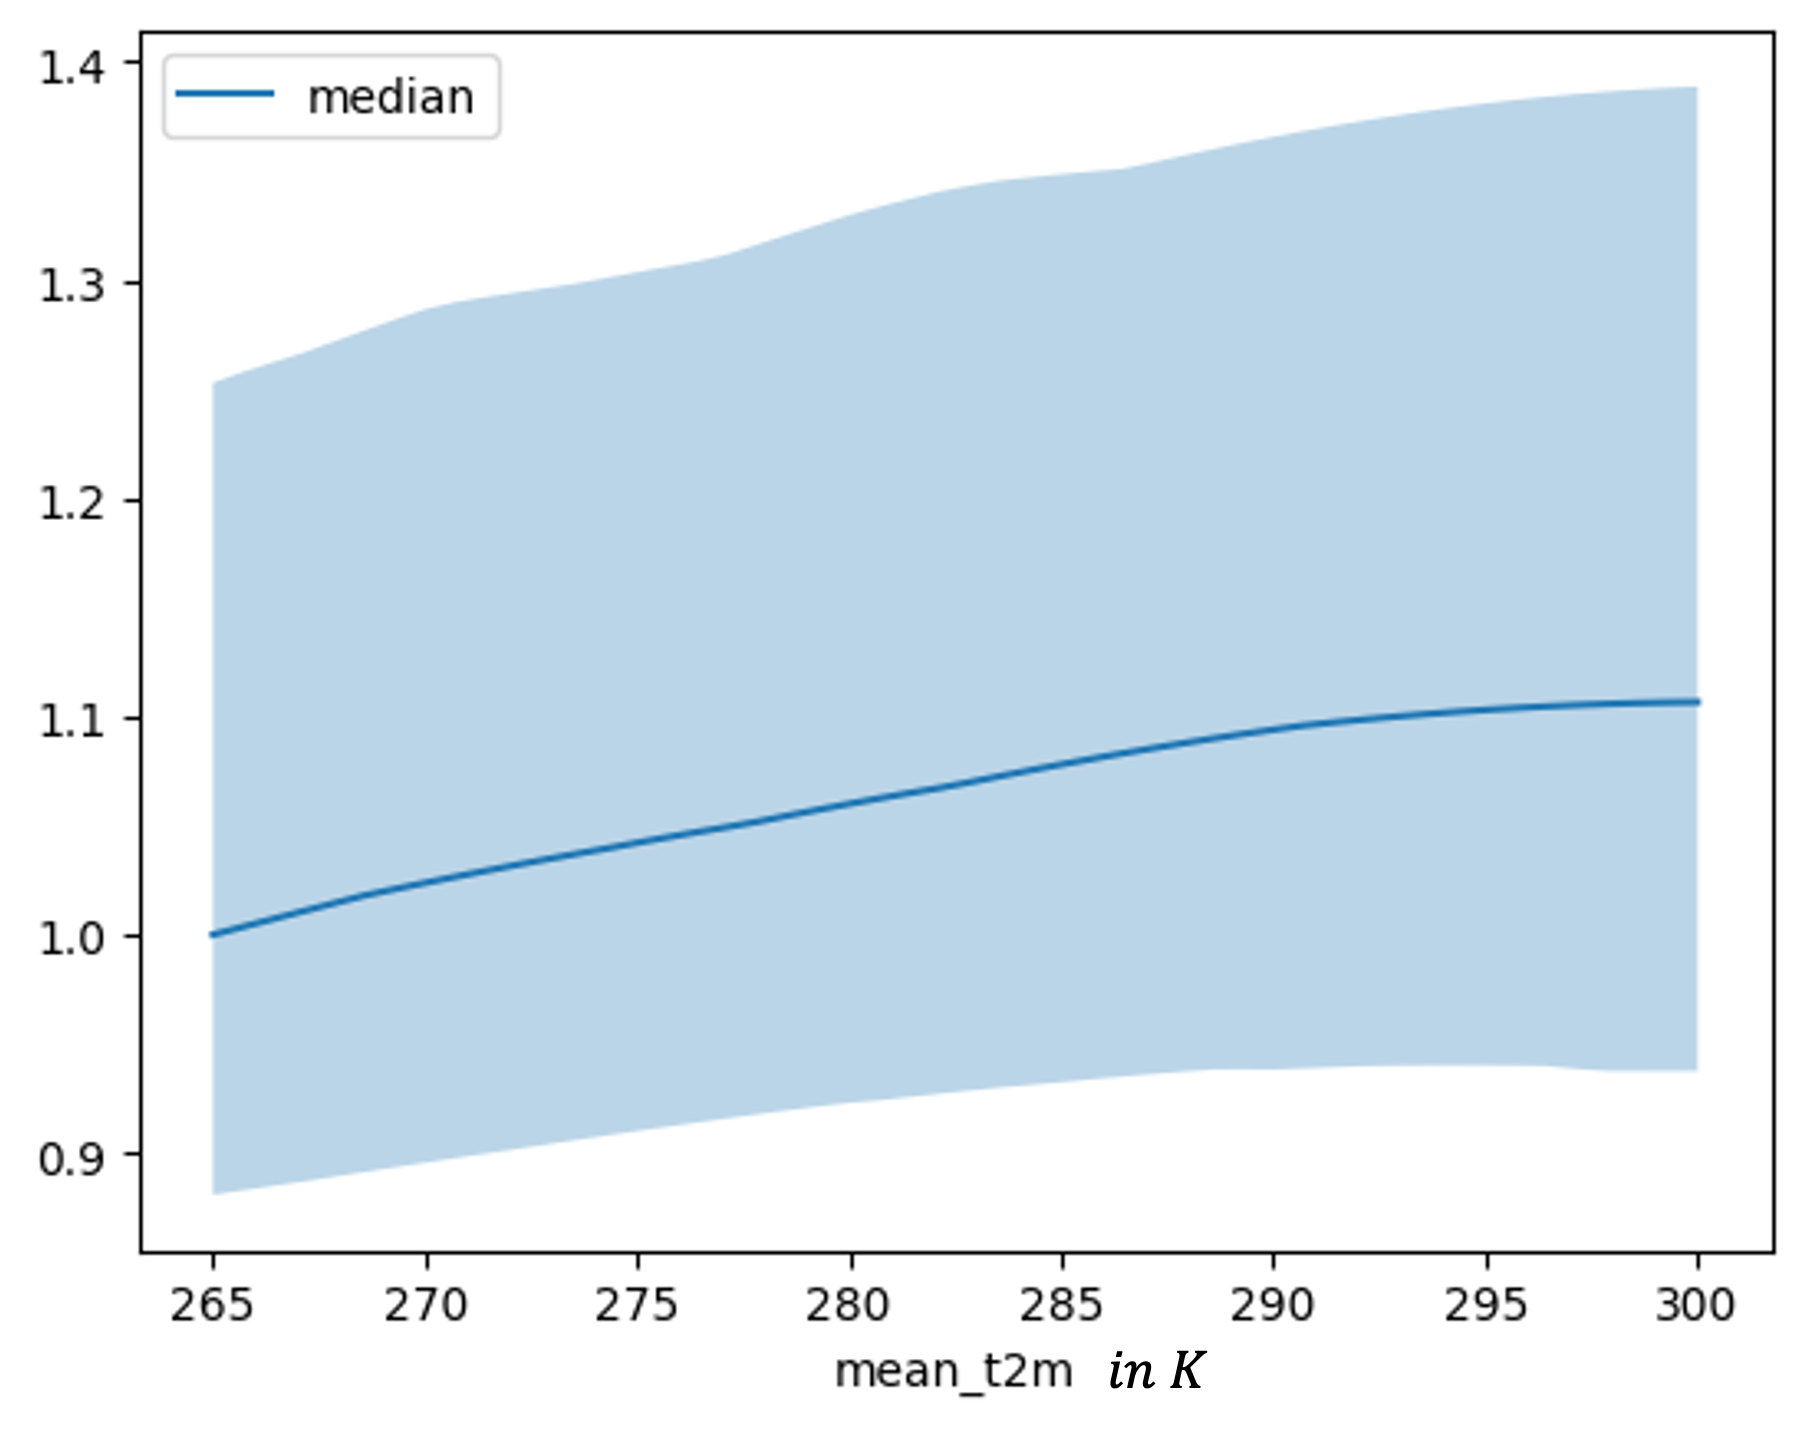
\includegraphics[width=0.7\linewidth]{work/07-hydroLSTM/images/mean_t2m_feature_importance_lstm} 

}

\caption{Feature dependence plot for mean two meter temperature for a lead time 5 trained LSTM}\label{fig:t2m-lstm-imp}
\end{figure}

\begin{figure}

{\centering 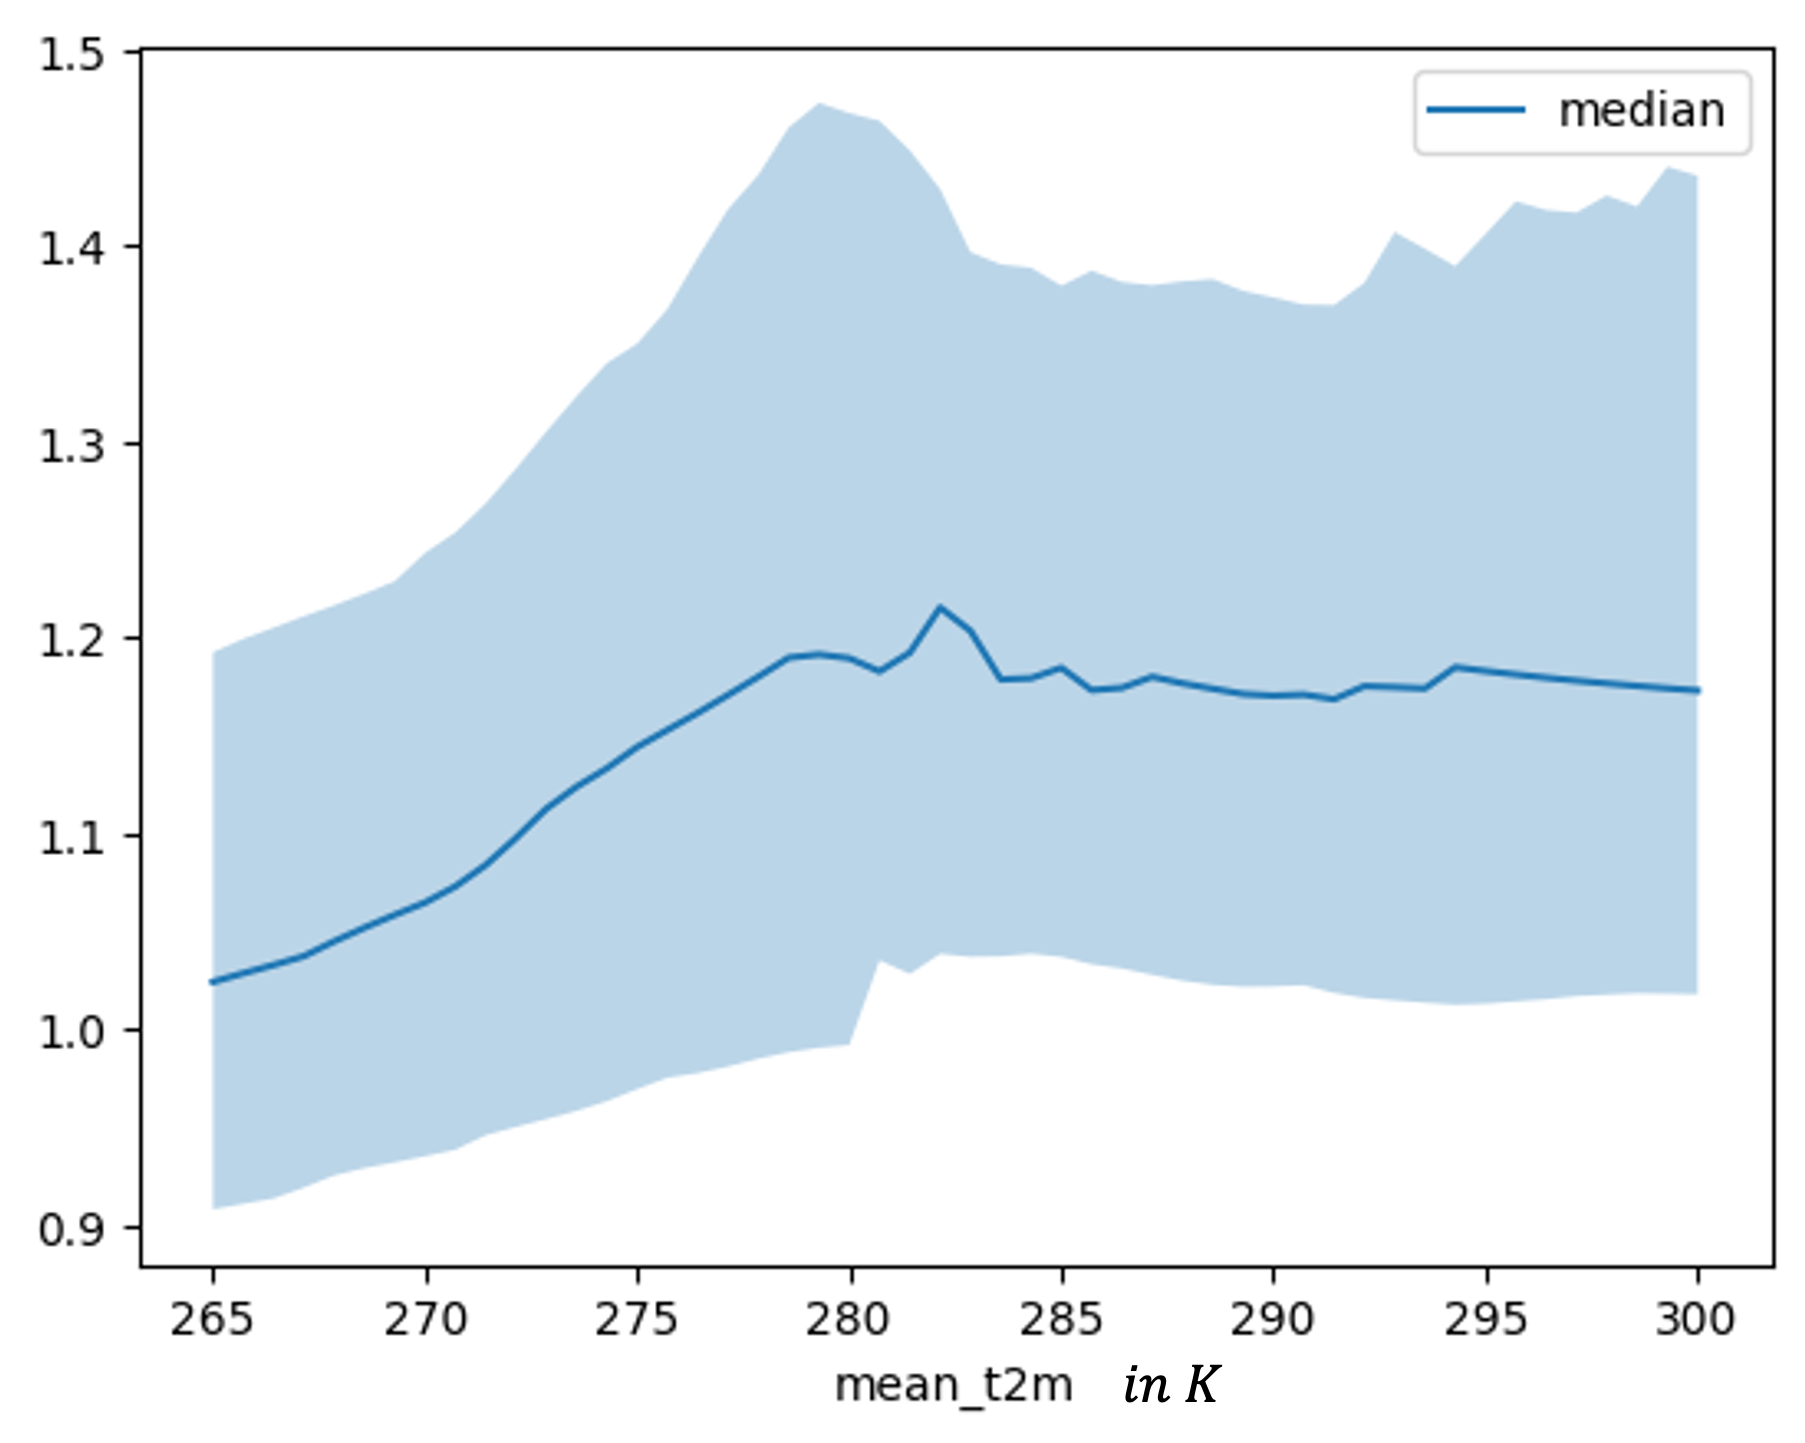
\includegraphics[width=0.7\linewidth]{work/07-hydroLSTM/images/mean_t2m_feature_importance_tft} 

}

\caption{Feature dependence plot for mean two meter temperature for a lead time 5 trained TFT}\label{fig:t2m-tft-imp}
\end{figure}

\section{Conclusion}\label{conclusion-2}

This study compares the performance of LSTM (Long Short-Term Memory) and Temporal Fusion Transformer (TFT) models in forecasting streamflows of the bavarian Regen river for up to seven days ahead, using precipitation and temperature as future known covariates alongside historical streamflow data. The data used was obtained from freely available data provided by the Bavarian hydrology authority and Copernicus Climate Project.

The findings indicate that both models exhibit limitations in predicting extreme values such as floods, with KGE (Kling-Gupta Efficiency) scores significantly lower than those reported in similar studies like \citet{sabzipour}, likely due to limited data amounts and the challenges inherent in modeling a river system instead of a reservoir. The results also demonstrate a clear difference in performance trends between the two models across different lead times.

Although the KGE was not used as the loss function in training the models. The LSTM's observed KGE scores are high starting at 0.9696 for a one-day lead time, before dropping sharply to 0.3185 for a seven-day lead time. Conversely, the TFT model shows a more gradual decline, from 0.8352 at one day to 0.5717 at seven days, suggesting it maintains more consistent accuracy over longer forecast horizons.

Despite the sharper decline in performance for longer lead times, the LSTM model is notably less resource-dependent, making it a viable option for scenarios where computational resources are limited. However, attempts to forecast streamflows without future known meteorological variables were unsuccessful, underscoring the importance of these covariates in achieving accurate predictions.

While the moving average was applied here, it is not advised to use this tool for streamflow forecasting. By reducing the peaks in the target variable it artificially boosts the predictive abitlity of the model and forces the model to miss the peaks by an even larger margin. In a flood scenario even with a high KGE, the model would miss the exact streamflow value as it was trained on lower peaks and would underestimate the posed danger in the situation.

\section{Outlook}\label{outlook}

Implementing a robust hyper-parameter tuning routine is essential to optimize model performance. This process will require additional computational resources due to the complexity and extensive search space. Given the high dependency of hyper-parameters on lag, it might be necessary to tune hyper-parameters for each lead time separately.

To make the models more sensitive to extreme events such as floods, specialized loss functions could be employed or training a consecutive model that that specifically forecasts the peaks taking the first models predictions as inputs.

The ERA5 dataset used for obtaining meterological data in this study only provides a very coarse representation of the underlying variables. The use of down scaling techniques to obtain a finer grid than the one used in this study might be able to boost the accuracy of the model.

Another next step could be to test the models ability to generalize by training on multiple datasets from different rivers. Including static variables such as river basin properties and land use information can help in creating a more comprehensive model that can adapt to various river systems.

\chapter{The Lancet Report 2023}\label{he1}

\emph{Author: Michael Strobl}

\emph{Supervisor: Prof.~Dr.~Helmut Küchenhoff}

\emph{Suggested degree: Bachelor}

\section{Introduction}\label{introduction-3}

The 2023 report of the Lancet Countdown on health and climate change (\citet{romanello20232023}) aims to monitor the evolving impact of climate change on health and the emerging health opportunities of climate action. It is in its eighth iteration and was created by 114 scientists and health practitioners from 52 research institutions and UN agencies from all continents (but Antarctica). While this chapter is based on the 2023 report, there are also regional reports available, such as the 2024 report for Europe (\citet{Van_Daalen2024-ut}).

The current report focuses on 47 indicators, tracking changes based on observed data as well as projections, in the following fields:

\begin{enumerate}
\tightlist
\item
  Health hazards, exposures, and impacts
\item
  Adaptation, planning, and resilience for health
\item
  Mitigation actions and health co-benefits
\item
  Economics and fincance
\item
  Public and political engagement with health and climate change
\end{enumerate}

The remainder of this chapter provides some background information on climate models, detailed information on three indicators, and a discussion.

\section{Background}\label{background}

Shared Socioeconomic pathways (SSPs) (\citet{RIAHI2017153}) were established by the climate research community in order to make the analysis of future climate impacts, vulnerabilities, adaptation, and mitigation possible. They describe alternative socioeconomic developments regarding their energy, land use, and emissions implications, e.g.~more or less renewable energy vs.~fossil fuels. The following SSPs are of interest for the rest of this chapter:

\begin{enumerate}
\tightlist
\item
  SSP1: Sustainability (low challenges to mitigation and adaption), corresponding to a 2°C emission scenario
\item
  SSP3: Regional Rivalry (high challenges to mitigation and adaptation), corresponding to a 3.7°C emission scenario
\end{enumerate}

These pathways are considered by climate models, e.g.~CMIP6 (\citet{gmd-9-1937-2016}), in order to describe multiple scenarios for climate projections. Figure \ref{fig:cmip6strobl} shows CMIP6 simulations for multiple models and all SSPs. In this chapter, we consider SSP1, representing a sustainable path, and SSP3, representing a non-sustainable path, which humanity is following right now.

\begin{figure}
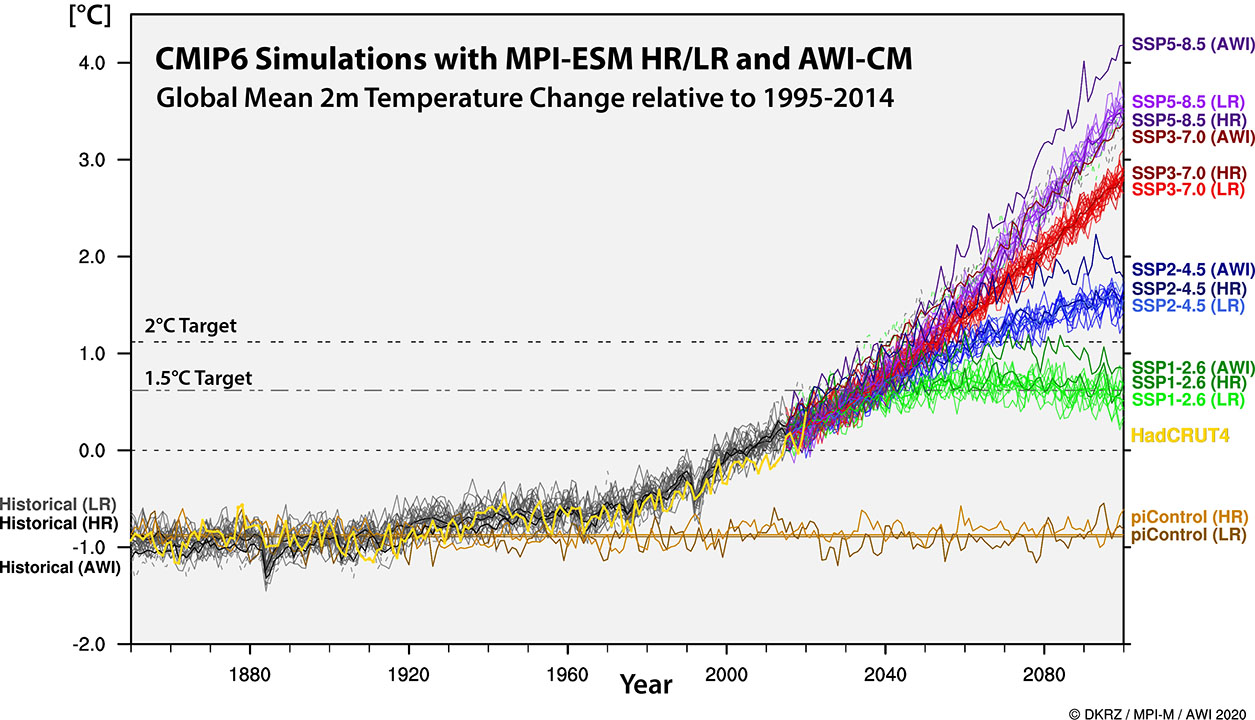
\includegraphics[width=1\linewidth]{work/08-lancet/figures/cmip6} \caption{CMIP6 climate simulations for SSPs with projections until 2100 (https://www.dkrz.de/en/communication/climate-simulations/cmip6-en/cmip6-acivities-at-dkrz-overview?set\_language=en; accessed on July 10, 2024)}\label{fig:cmip6strobl}
\end{figure}

\section{Selected Indicators}\label{selected-indicators}

We selected three indicators from the first field (Health hazards, exposures, and impacts) with detailed descriptions and outcomes.

\subsection{Indicator 1.1.2: Exposure of vulnerable populations to heatwaves}\label{indicator-1.1.2-exposure-of-vulnerable-populations-to-heatwaves}

Heatwaves have a severe or even life-threatening impact on human health, e.g.~high temperatures can cause heat stroke, heat exhaustion, heat syncope, and heat cramps (see, for example, \citet{doi:10.1161/CIRCULATIONAHA.122.061832} or \citet{chambers2020}). The following variables (among others) can influence mortality: increased risk for older adults (\textgreater65 years of age), low-income countries due to a reduced number of health workers, or pre-existing cardiovascular and chronic respiratory conditions.

This indicator tracks the number of heatwave days and the exposure of vulnerable populations (older adults and infants \textless1 years of age) to heatwaves. A heatwave day is a period of 2 or more days where both the minimum and maximum temperatures are above the 95th percentile of temperatures in 1986-2005.

The following datasets were used for this indicator:

\begin{itemize}
\tightlist
\item
  ERA5 monthly averaged data on single levels (\citet{hersbach2020era5}): World-wide weather data on a lat-lon grid of 0.25 degrees from 1940 onwards.
\item
  ISIMP3b Bias Adjustment dataset (\citet{lange2021isimip3b}): A bias adjusted and downscaled version of the output of CMIP6 climate models with projections up to the year 2100.
\item
  Hybrid gridded demographic data for the world (\citet{Chambers_2020}): Demographics data from 1950-2020 with 5-year population bands and a 0.5 degree grid.
\item
  2020 Revision of World Population Prospects (\url{https://population.un.org/wpp/}): This dataset contains population estimates as well as projections for 237 countries or areas between 1950 and 2100.
\item
  A global downscaled age structure dataset for assessing human impacts of climate change (\citet{briggsdaviddownscaled}): This dataset contains historic population estimates starting in 1970 and projections considering SSP1 and SSP3 in a 0.5 degree grid.
\end{itemize}

Headline Finding:

``In 2013-2022, infants and people over 65 experienced, on average, 108\% more days of heatwave per year than in 1986-2005.''

Figures \ref{fig:heatwaves1infantsstrobl} and \ref{fig:heatwaves1adultsstrobl} show the increase in the number of heatwave days, comparing the time periods 1986-2005 and 2013-2022, for infants and older adults, respectively. This increase (or decrease for Portugal) per country can be calculated, for example, through ERA5 monthly averaged weather data and the hybrid gridded demographics dataset.

\begin{figure}
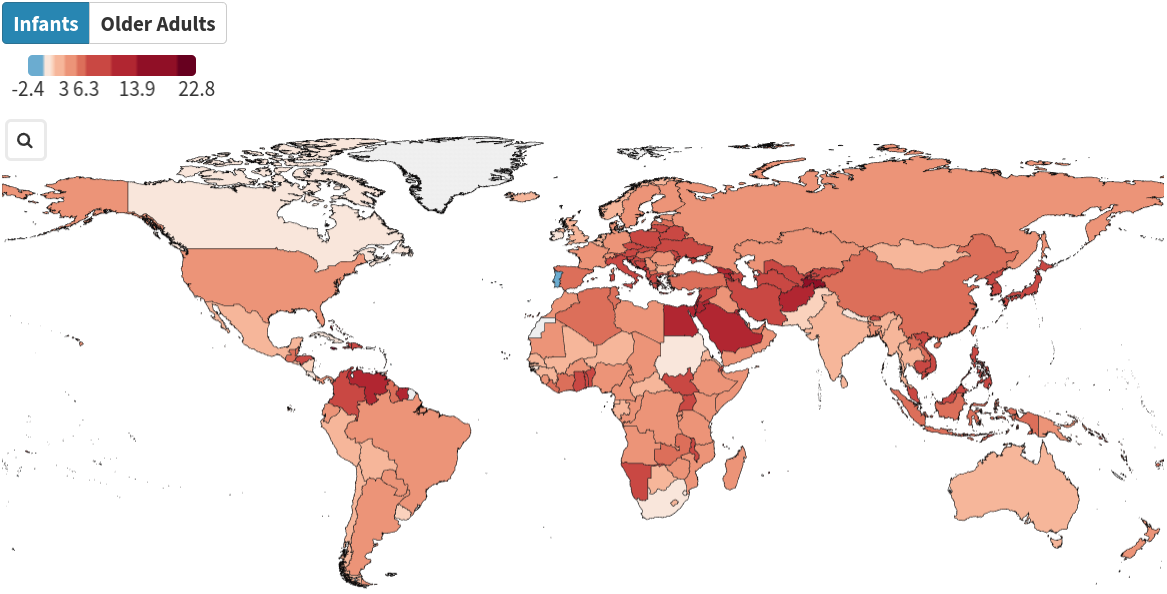
\includegraphics[width=1\linewidth]{work/08-lancet/figures/indicator_1_1} \caption{Change in number of heatwave days per country for infants, comparing the time periods 1986-2005 and 2013-2022.}\label{fig:heatwaves1infantsstrobl}
\end{figure}
\begin{figure}
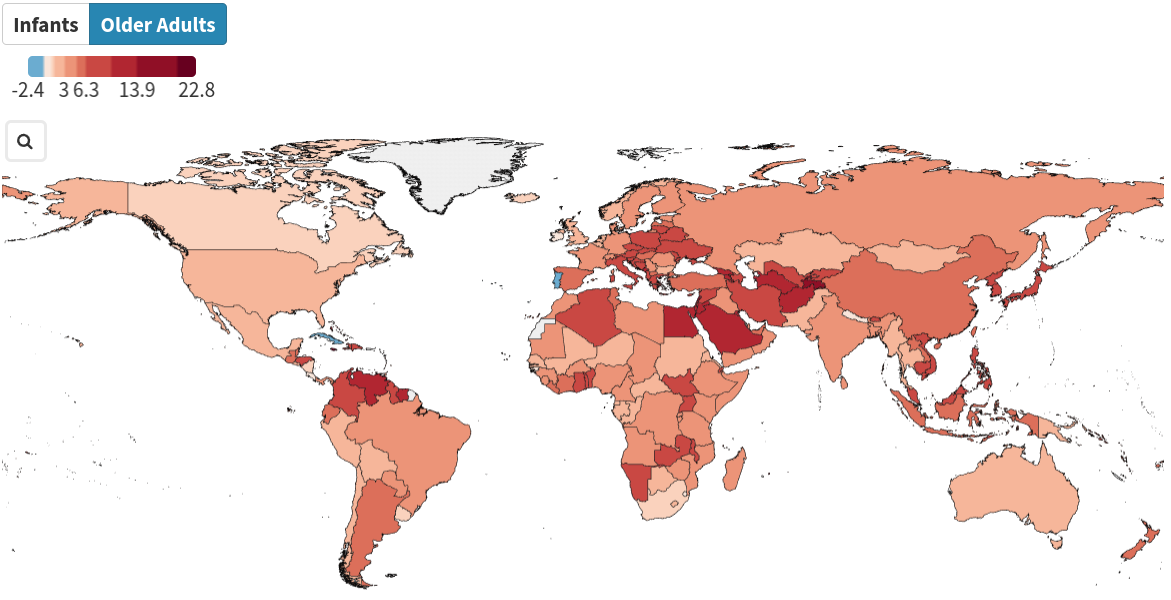
\includegraphics[width=1\linewidth]{work/08-lancet/figures/indicator_1_2} \caption{Change in number of heatwave days per country for older adults, comparing the time periods 1986-2005 and 2013-2022.}\label{fig:heatwaves1adultsstrobl}
\end{figure}

The change in the number of heatwave days ranges from approximately -1 in Portugal to 16 in Tajikistan, with only minimal differences between infants and older adults.

Similarly, the ISIMP3b Bias Adjustment dataset combined with the global downscaled age structure dataset can be used to project the change in heatwave days up until the year 2100. Figures \ref{fig:heatwaves2ssp1strobl} and \ref{fig:heatwaves2ssp3strobl} show the projected change in heatwave days for older adults at mid-century (2041-2060) with baseline period 1995-2014. For example, the increase for Venezuela ranges from approximately 88 (SSP1) to 153 (SSP3) heatwave days per year.

\begin{figure}
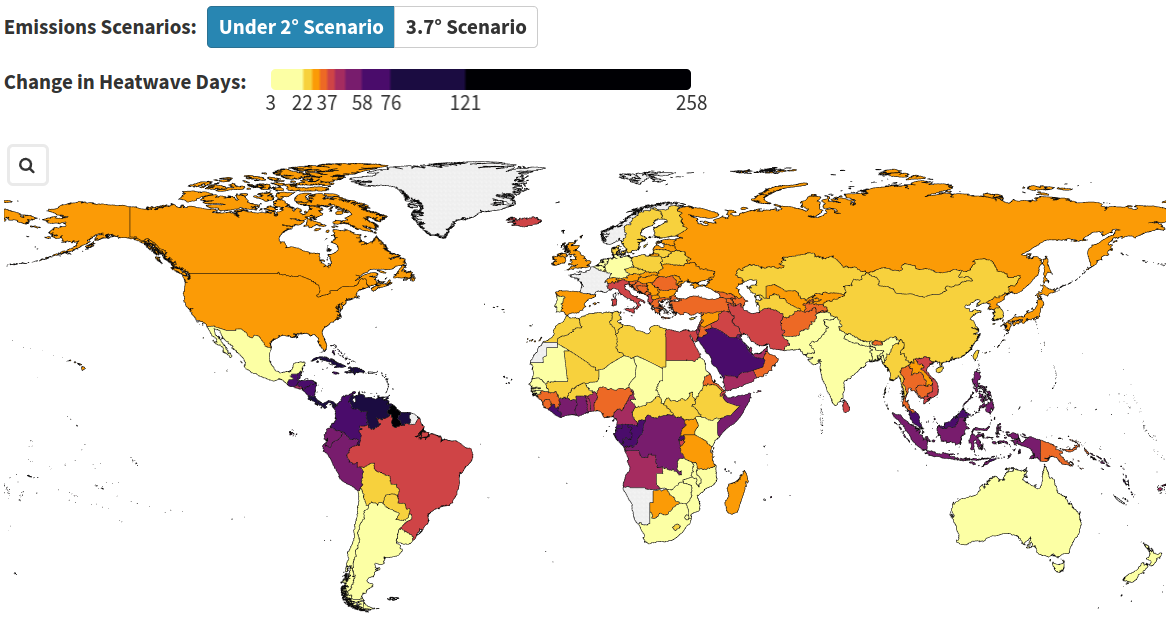
\includegraphics[width=1\linewidth]{work/08-lancet/figures/indicator_1_3} \caption{Projections of the change in number of heatwave days for older adults per country for SSP1 (under 2 degree scenario) for mid-century (2041-2060) with baseline period 1995-2014.}\label{fig:heatwaves2ssp1strobl}
\end{figure}
\begin{figure}
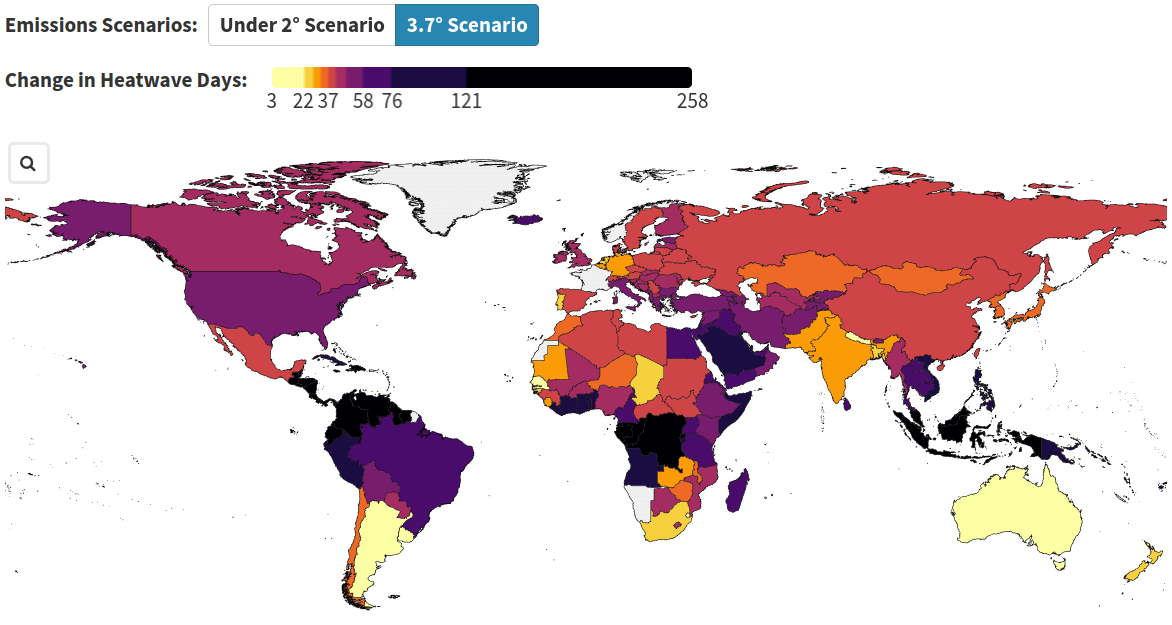
\includegraphics[width=1\linewidth]{work/08-lancet/figures/indicator_1_4} \caption{Projections of the change in number of heatwave days for older adults per country for SSP3 (3.7 degree scenario) for mid-century (2041-2060) with baseline period 1995-2014.}\label{fig:heatwaves2ssp3strobl}
\end{figure}

\subsection{Indicator 1.1.5: Heat-related mortality}\label{indicator-1.1.5-heat-related-mortality}

This indicator is tracking days with temperatures exceeding safe levels for humans and heat-related mortality. Only older adults are considered.

Similar datasets are used here as for the previous indicator. However, the difficulty arises due to the fact that safe temperatures may vary across regions (see \citet{Honda2014}).

Headline Finding:

``In 2018-2022, people experienced on average 86 days of health-threatening high temperatures annually. 60\% of such temperatures were made more than twice as likely to occur by human-caused climate change.''

Therefore, \citet{Honda2014} created the notion of an Optimum Temperature (OT), at which the mortality is the lowest. Figure \ref{fig:mortalityhondastrobl} shows an example for the Tokyo Prefecture and the period 1972-2008. A smoothing spline with six degrees of freedom was used to model the Relative Risk (RR) for mortality and observed daily maximum temperature data. OT represents the daily maximum temperature where RR is the lowest. RR was used here in order to account for different populations of regions and an RR=1.0 is the reference mortality at around OT, i.e.~the average number of deaths observed when the daily maximum temperature was within the range of the 75th to the 85th percentile for each year.

\begin{figure}
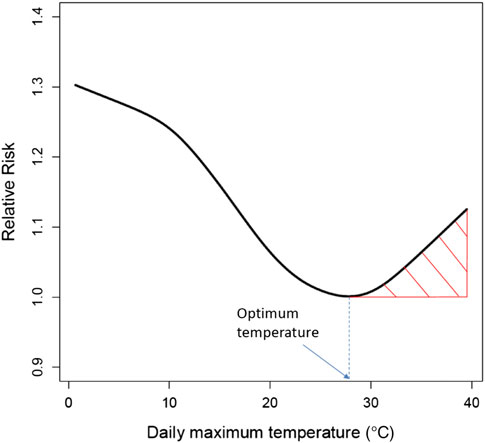
\includegraphics[width=1\linewidth]{work/08-lancet/figures/121_3} \caption{A smoothing spline with six degrees of freedom was used for temperature data from the Tokyo Prefecture and the period 1972-2008, showing the daily maximum temperatures and the Relative Risk (RR) for mortality.}\label{fig:mortalityhondastrobl}
\end{figure}

The shaded area to the right of OT represents temperatures with increased mortality, i.e.~daily maximum temperatures above OT are considered as risky for older adults. The average OT percentile of 47 Japanese prefectures was 83.6, which was used to decide which daily maximum temperatures exceeded safe levels for this indicator. In addition, a distributed lag nonlinear model (\citet{Armstrong2006-mv}) was used to model the increase in mortality (represented by RR) depending on temperature. This model is considered as a response function, which can be used to calculate the RR and therefore the absolute increase of mortality depending on the observed or projected temperatures.

Figure \ref{fig:mortality1strobl} shows the increase in the number of days with unsafe temperatures (daily maximum temperatures exceeding OT). This includes the increasing number of days that were made at least twice as likely due to human induced climate change (it is not described how the red line was created).

\begin{figure}
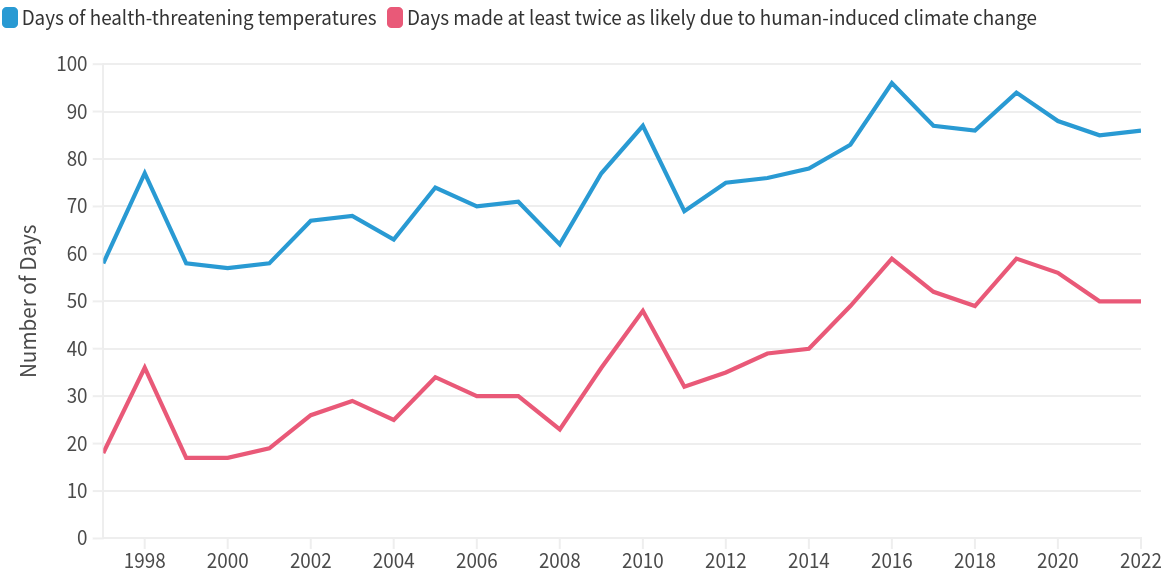
\includegraphics[width=1\linewidth]{work/08-lancet/figures/indicator_2_1} \caption{Average number of days with unsafe temperatures for older adults from 1997 to 2022, including days that are twice as likely due to climate change.}\label{fig:mortality1strobl}
\end{figure}

In addition, Figures \ref{fig:mortality2ssp1strobl} and \ref{fig:mortality2ssp3strobl} show the absolute projected increase in heat-related mortality per country for older adults at mid-century (2041-2060) compared to 1995-2014 as baseline, for SSP1 and SSP3, respectively. In both cases there is an increase, although it seems that the two scenarios, SSP1 and SSP3, have been flipped accidentially. In addition, only the absolute increase is shown, i.e.~it is obvious that highly populated countries, such as India and China, have a very high increase compared to smaller countries.

\begin{figure}
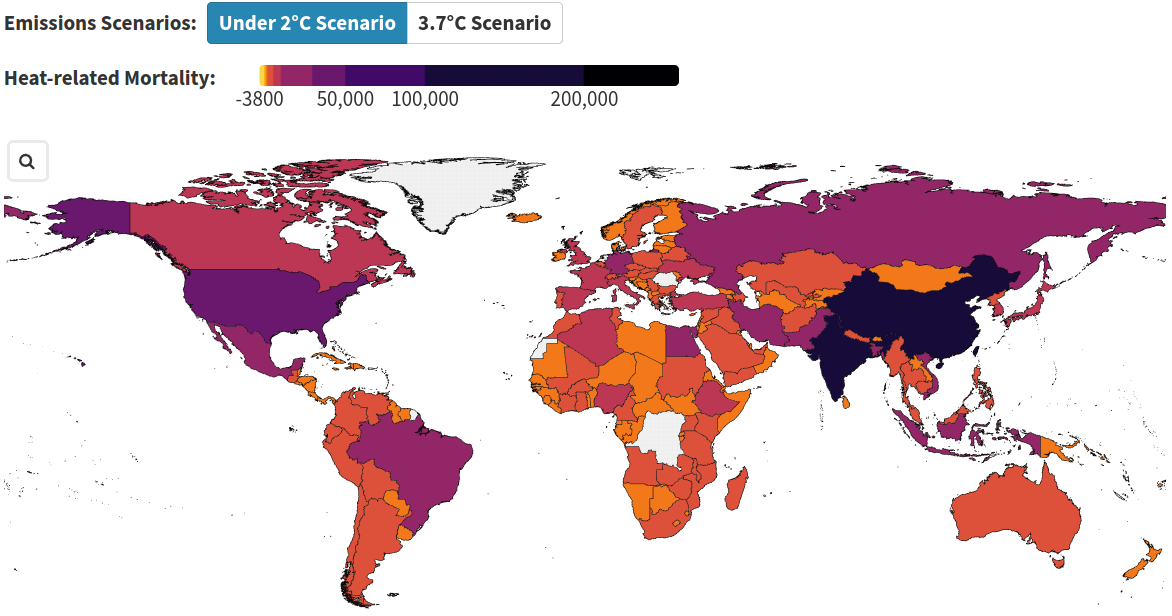
\includegraphics[width=1\linewidth]{work/08-lancet/figures/indicator_2_4} \caption{Projections of the absolute change in heat-related mortality for older adults per country for SSP1 (under 2 degree scenario) for mid-century (2041-2060) with baseline period 1995-2014.}\label{fig:mortality2ssp1strobl}
\end{figure}
\begin{figure}
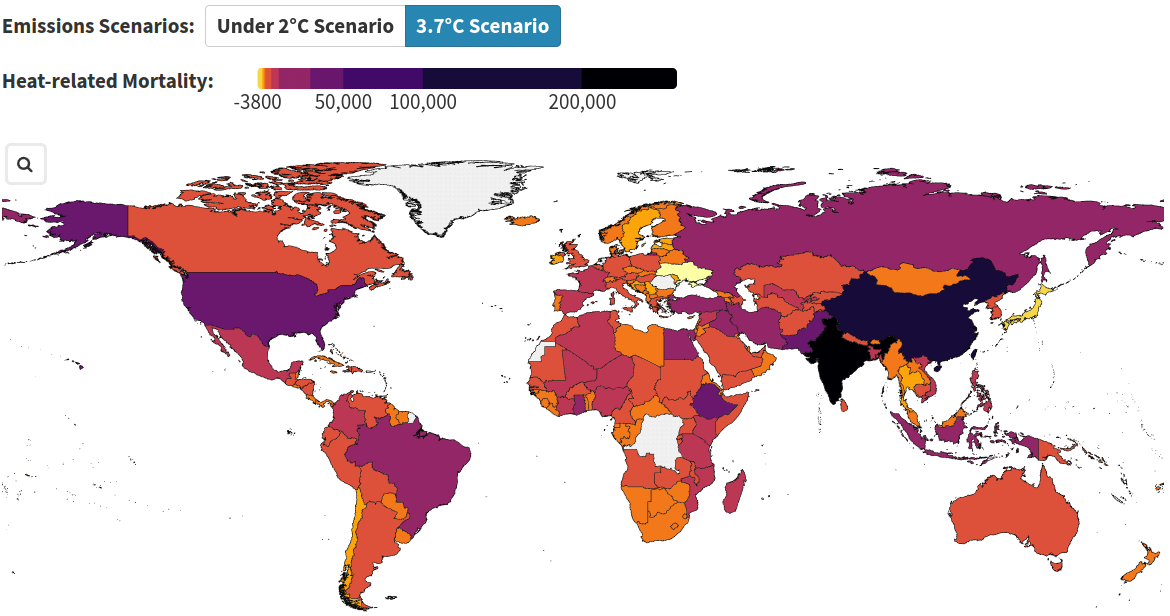
\includegraphics[width=1\linewidth]{work/08-lancet/figures/indicator_2_5} \caption{Projections of the absolute change in heat-related mortality for older adults per country for SSP3 (3.7 degree scenario) for mid-century (2041-2060) with baseline period 1995-2014.}\label{fig:mortality2ssp3strobl}
\end{figure}

The response function is kept constant for these projections, i.e.~adaptation is ignored for this indicator. Also, absolute numbers of mortality are used here, i.e.~it was not distinguished between heat-related deaths and other causes.

\subsection{Indicator 1.4: Food insecurity and undernutrition}\label{indicator-1.4-food-insecurity-and-undernutrition}

In 2022, 725 million people faced hunger and in 2021, 3.1 billion people were unable to afford a healthy diet (\citet{noauthor_2023-jt}). For example, climate change is undermining crop yields, affecting labour capacity, and threatening food security of marine resources.

In addition to the previously mentioned datasets, specifically ERA5 and ISIMP3b, data from the Food and Agriculture Organization Food Insecurity Experience Scale (FIES) (\citet{CAFIERO2018146}) was used. This dataset contains survey data from 153 countries and territories during the years 2014, 2015, and 2016. Among others, people were asked for whether they experienced moderate or severe food insecurity within the past 12 months. This was matched with weather data in these peoples specific regions in order to find out whether they experienced heatwaves (as previously defined) or drought months (12-monthly SPEI; only during the growth season of specific crops). In order to make predictions for all other years, including the future, a time-varying panel regression model was used (without further detail). The goal was to predict the percentage of people reporting food insecurity based on heatwaves and drought months experienced within a specific year.

Headline Finding:

``The higher frequency of heatwave days and drought months in 2021 compared to 1981--2010, is associated with 127 million more people experiencing moderate or severe food insecurity.''

Figure \ref{fig:food1strobl} shows world-wide predictions of the change in percentage points (using the previously mentioned model) for heatwaves and drought months for the period 2014-2021. As temperatures, number of heatwave days as well as number of drought months increase, more people are expected to experience severe or moderate food insecurity.

\begin{figure}
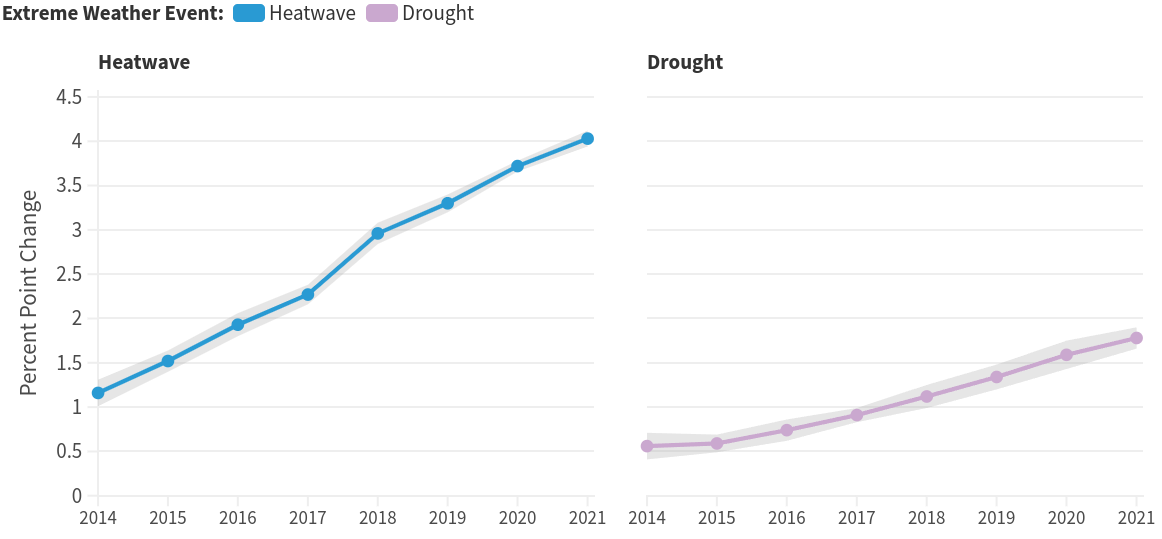
\includegraphics[width=1\linewidth]{work/08-lancet/figures/indicator_3_1} \caption{Impact of extreme weather (heatwaves and droughts) on food insecurity from 2014-2021, based on survey data.}\label{fig:food1strobl}
\end{figure}

Figures \ref{fig:food2ssp1strobl} and \ref{fig:food2ssp3strobl} show projections (SSP1 and SSP3, respectively) for the percentage point changes for both kinds of extreme weather combined for mid-century (2014-2060), compared to the baseline 1995-2014. For example for Somalia, this change ranges from 4.02 (SSP1) to 10.32 (SSP3).

\begin{figure}
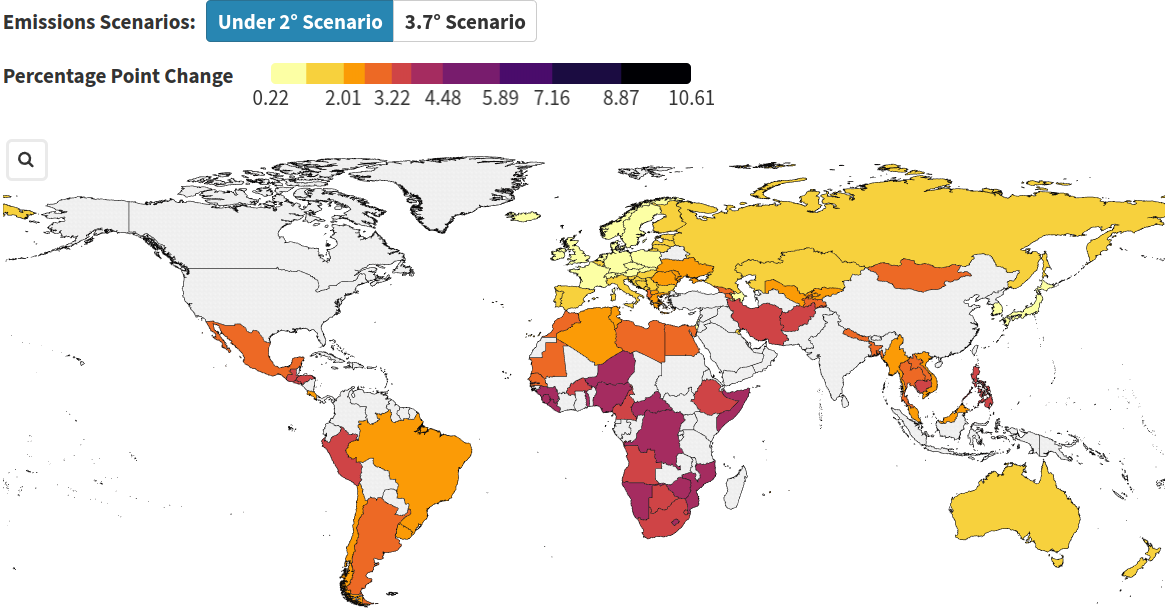
\includegraphics[width=1\linewidth]{work/08-lancet/figures/indicator_3_2} \caption{Projections of the impact of extreme weather on food inscurity per country for SSP1 (under 2 degree scenario) for mid-century (2041-2060) with baseline period 1995-2014.}\label{fig:food2ssp1strobl}
\end{figure}
\begin{figure}
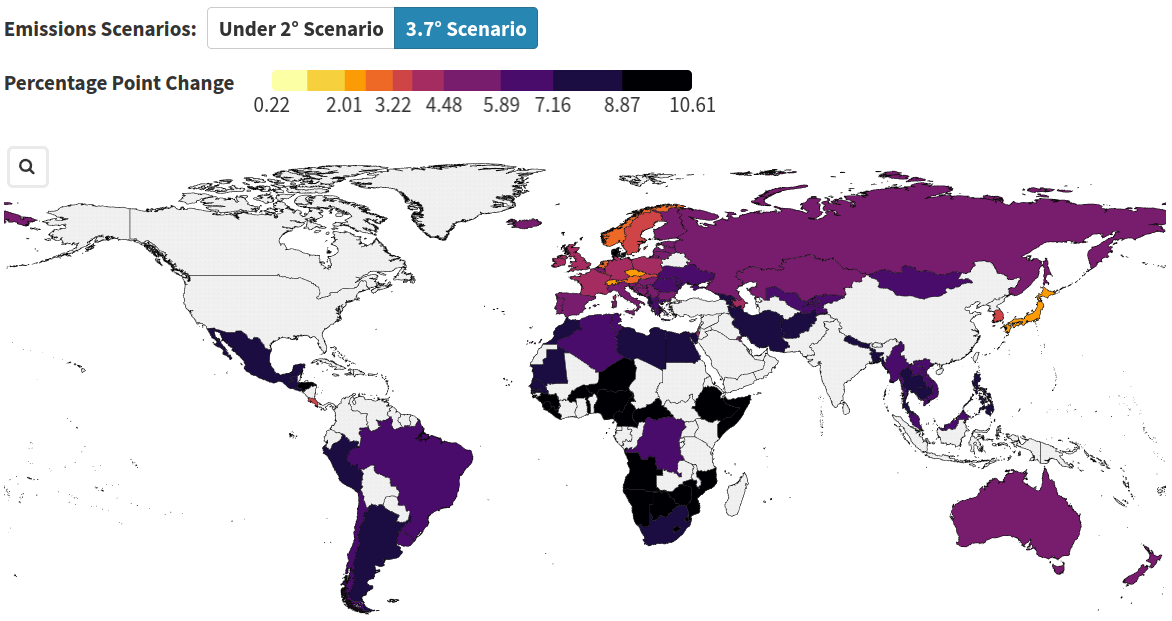
\includegraphics[width=1\linewidth]{work/08-lancet/figures/indicator_3_3} \caption{Projections of the impact of extreme weather on food inscurity per country for SSP3 (3.7 degree scenario) for mid-century (2041-2060) with baseline period 1995-2014.}\label{fig:food2ssp3strobl}
\end{figure}

It is unclear why for many countries there is missing data.

\section{Discussion}\label{discussion}

The 2023 report of the Lancet Countdown on health and climate change provides a comprehensive overview of the current state of the impact of climate change on health and opportunities of climate action. 47 indicators are used to keep track of where humanity is at right now.

We provided detailed descriptions of three main indicators and the modelling techniques used, if mentioned. However, there are a few issues discovered:

\begin{itemize}
\tightlist
\item
  These modelling techniques are typically not described in much detail. Sometimes, as in the case for \citet{Honda2014}, some more information is provided in cited articles, but still on a relatively high level.
\item
  The baselines for comparisons or projections vary. It is not clear, nor described, why different baselines are used. For projections, it is obvious that the baseline for CMIP6 projections (1995-2014) was used, without information on why not the one that was previously used for the indicator at hand.
\item
  In general, the main findings are reported, without going much into detail on how the authors came up with these. In some cases, e.g.~indicator 1.1.5, cited articles provide more information, but in other cases, e.g.~indicator 1.4, it seems to be mainly the authors own work, without providing details.
\end{itemize}

\chapter{Epidemiologic studies on the heat effects}\label{he2}

\emph{Author: Author}

\emph{Supervisor: Helmut Kuechenhoff}

\emph{Degree: Bachelor}

There are many epidemiological studies for assessing the effect of heat on health.
One strategy is to use daily mortality data and weather data in certain areas to
estimate heat related mortality by regression models. Two recent papers by groups of
researchers give an overview:

\begin{enumerate}
\item
  General effects
  \citet{masselot}
\item
  Joint effects of air pollution and heat
  \citet{stafoggia}
\end{enumerate}

Results and statistical methods should be presented

\chapter{Controversial issue : heat and humidity}\label{he3}

\emph{Author: Mona Niethammer}

\emph{Supervisor: Helmut Kuechenhoff}

\emph{Degree: Master}

\section{Abstract}\label{abstract-3}

As climate change progresses, heat-related mortality and adverse health outcomes are also increasing. In the chapters before it was mainly talked about temperature related outcomes. This chapter focuses on heat events and how humidity plays a crucial role in high ambient temperatures and the effect on health outcomes. Physiological research indicates that both heat and humidity significantly impact the body's response to heat. Thus, influencing mortality and adverse health outcomes. Several epidemiological studies aimed to show this relationship, found however only minimal or even no effect of humidity on negative health outcomes. This discrepancy between physiological knowledge and epidemiological findings creates a, as (\citet{bald}) describes it, controversial issue. This will be further explored in this chapter.

\section{Introduction}\label{introduction-4}

\subsection{Background}\label{background-1}

Climate change is a broad and pressing topic as the number of heat-related deaths and the air-temperature break records. Extreme heat waves have become a consistent feature of summer seasons, leading to an increase in heat-related fatalities (\citet{ebi}). Rising greenhouse gas concentrations further contribute to rising temperatures and humidity at the same time. Physiological knowledge indicates that heat and humidity both contribute to human heat stress, adversely affecting the human body (\citet{bald}). Heat stress occurs when environmental conditions overwhelm the body`s cooling mechanism (\citet{buzan}). When the body is not able to sufficiently lower its core temperature, the human body suffers health problems, potentially leading to death. From a physiological perspective, the body's cooling mechanisms are clearly influenced both by heat and humidity.

In contrast, a wide range of epidemiological studies have found either no or only a weak correlation between humidity and human heat stress or adverse health outcomes. Those studies all infer that a rise in air-temperature (heat) is associated with negative health outcomes. These two contradictions lead, according to (\citet{bald}), to a controversial issue as physiologically it is known that there is an effect of humidity on health outcomes, whereas in epidemiological studies they did not find evidence for such an effect. Figure 1 describes this contradiction between physiological knowledge and epidemiological studies. Heat in this chapter is used as synonym for high ambient temperature.

\begin{center}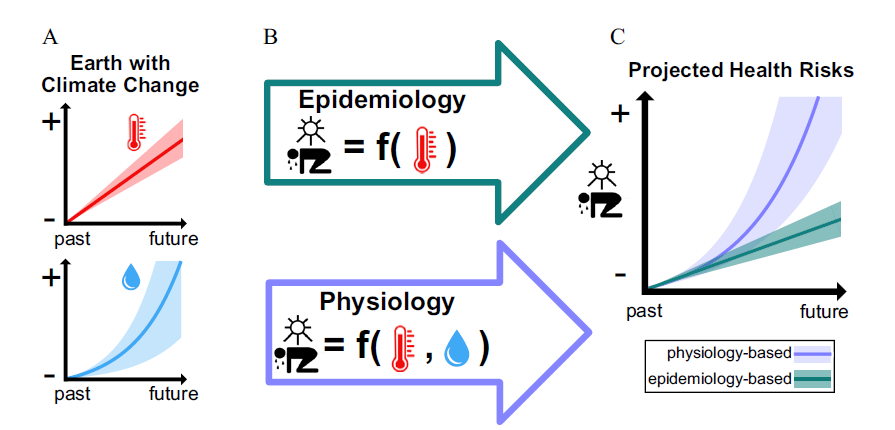
\includegraphics[width=0.8\linewidth]{Controversial Issue} \end{center}

\textbf{Figure 1:} Flowchart illustrating the controversial issue between epidemiological studies and physiological knowledge.\\
\emph{A: illustrates how heat and humidity changes with climate change. B: illustrates that epidemiological studies only take heat as driver into account, the physiological view heat and humidity. C: shows the predictions from an epidemiological and physiological view.}

\subsection{Epidemiological Studies}\label{epidemiological-studies}

Numerous epidemiological studies investigated the influence of heat and humidity on negative health outcomes such as death or cardiovascular diseases. Results of these studies are mixed regarding the association of humidity and negative health outcomes. As an example, a study in New York, conducted by Barreca found a positive correlation between high levels of relative humidity (RH) and cardio-respiratory hospitalizations. However, this study is one of few that identified an effect of humidity on negative health outcomes.
Baldwin et al.~reviewed several epidemiological studies and conducted further research. They concluded six key reasons why epidemiological studies found less or even no effect of humidity on health outcomes:

\begin{enumerate}
\def\labelenumi{\arabic{enumi})}
\tightlist
\item
  At high temperatures, humidity has minimal or even no influence on negative health outcomes\\
\item
  Study results may be skewed by limited data sets\\
\item
  Analyses often focus on vulnerable populations, like elderly, infants or individuals with impaired sweating functions\\
\item
  Necessary extreme values of heat and humidity to show a significant impact on heat strain are rare\\
\item
  The relationship between heat and humidity is often not adequately considered. This may lead to inappropriate model results\\
\item
  Sub-daily meteorological phenomena, such as rain, which occur during high heat and humidity, may bias studies based on daily data\\
  (\citet{bald}).
\end{enumerate}

\subsection{Physiological knowledge}\label{physiological-knowledge}

Physiological evidence indicates that heat and humidity increase health risks, leading to higher rates of morbidity, mortality, reduced physical work capacity, and other adverse health outcomes as the climate crisis worsens. (\citet{buzan})

The human body has two primary cooling mechanism to control the body temperature. One mechanism redistributes the blood flow to the skin (vasodilation), and therefore allows metabolically generated heat from inside of the body to reach the skin's surface and subsequently the environment. This process requires an increased blood flow and elevates cardiac demand. This may trigger cardiovascular events such as myocardial infarction in subjects with heart conditions.
The second mechanism involves secreting sweat onto the skin. Subsequently, the sweat evaporates to the environment and heat from the body is removed. These two mentioned cooling mechanisms are crucial for the human body to maintain a sustainable core temperature. (\citet{ebi})

The effectiveness of these cooling mechanisms decline with the increase of heat and humidity. A higher ambient humidity reduces the proportion of sweat that evaporates from the skin into the air. Hence, the effectiveness of sweating decreases and sweating does not lead to heat loss anymore, causing a rise in body temperature. The human body responds to such ineffective sweating by an even higher rate of sweating. This can lead to heat stroke, dehydration, or the body's physical limits may simply be exceeded. (\citet{bald})

Certain populations are at higher risk due to less efficient cooling mechanisms. For instance, people older than 65 years may have a reduced sweating ability same as individuals with cardiovascular diseases who cannot effectively increase blood flow to the skin. These factors, among others, exacerbate the difficulty in cooling the body. (\citet{ebi})\\
When the body can no longer cool itself, heat stress occurs. However, these physiological insights are not consistently reflected in epidemiological studies. Several methodological and physiological factors might explain this discrepancy.

Firstly, heat-vulnerable individuals often have impaired sweating capacities, especially with aging this capacity decreases. Thermoregulatory sweating can decrease by up to 25\% in individuals older than 60. Consequently, they will be less sensitive to high humidity. Since most studies only include individuals over 65 years, this might explain the lack of association between humidity and heat stress.

Secondly, it is possible that the threshold at which differences in humidity impact the body's regulatory mechanisms are rarely attained. This means, that only at a specific threshold of humidity the body's cooling mechanisms have trouble and this threshold may be reached rarely in especially dry areas.

Thirdly, heat-related outcomes may result from other causes unrelated to humidity. For example, cardiovascular diseases are a leading cause of death, and high temperatures can exacerbate these conditions independently of humidity.

Lastly, dehydration, a major cause of heat-related deaths, reduces the amount of sweat, thereby minimizing the impact of high humidity on evaporation and cooling. (\citet{bald})

\section{Heat and Humidity in Studies}\label{heat-and-humidity-in-studies}

\subsection{Humidity definitions}\label{humidity-definitions}

Humidity has multiple definitions. This makes it crucial to select an appropriate measure to answer specific research questions. (\citet{bald}) categorize humidity variables into the four following groups:

\begin{enumerate}
\def\labelenumi{\arabic{enumi}.}
\tightlist
\item
  Simple relative variables including Relative Humidity (RH), Dew-point depression (DPD) and Saturation deficit.\\
\item
  Mass-based variables including specific humidity, absolute humidity, dew point temperature, vapor pressure and mixing ratio.\\
\item
  Composite indicators such as the Heat index, Humidex, Wet-bulb-temperature, UTCI and further more.\\
\item
  Physiologic-based humidity indicators including maximum evaporation, required evaporation, total evaporation.
\end{enumerate}

The simple relative variable RH (\%) is the ratio of actual vapor pressure (e) in the air to the saturation vapor pressure (\(e_s\)), indicating proximity to saturation (\(RH=e/e_s\)). The dew-point depression (DPD) (°C) indicates the relative dryness of the air and is the difference between the near-surface air temperature (\(T_a\)) and the dew point temperature (\(T_d\)) (\(DPD=T_a-T_d\)). Saturation deficit refers to the amount by which the water vapor must be increased in a given environment to reach saturation, assuming unchanged temperature and pressure.

The mass-based variable specific humidity (q) (g/kg) is the ratio of the mass of water vapor (g) to the total mass of moist air (kg). Absolute humidity is the density of water vapor, defined as the ratio of the mass of water vapor (g) to the volume of the air mixture (\(m^3\)). The dew point temperature (\(T_d\)) (°C) is the temperature at which saturation occurs. The mixing ratio (w) refers to the ratio of the mass of water vapor (g) to the mass of dry air (kg).

The Heat Index (HI) describes a ``feels like'' temperature, while the Humidex is a discomfort index. The wet-bulb temperature is the temperature at which air becomes saturated through evaporation at constant pressure. The Universal Thermal Climate Index (UTCI) (°C) is a physiologically based thermal stress scale designed to reflect the average human physiological response to the outdoor thermal environment.

The physiological-based humidity indicator maximum evaporation (\(E_{max}\)) represents the maximal evaporation rate in a given environment and clothing conditions. The required evaporation (\(E_{req}\)) measures the evaporation needed to achieve thermal balance, and the total evaporation (E) is the total amount of heat lost via evaporation of sweat from the body.

Davis et al.~reviewed the use of humidity variables in epidemiological studies. They found that 62\% of the studies used RH, while absolute and specific humidity were used in only 5.3\% and 1.5\% of the studies, respectively. They discussed the appropriate use of different humidity variables, especially the use of RH due to its strong inverse correlation with temperature and its diurnal and seasonal variability was mentioned. It is recommended to use RH sparingly. Instead, they recommend using mass-based variables such as absolute or specific humidity, as they provide a more accurate measure of exposure to humidity levels.\\
The selection of humidity variables must be done carefully, they can be highly correlated with other variables, for example with heat. Davis et al.~concluded that using RH as humidity variable is often inappropriate and should be done with caution if necessary. (\citet{davis})

The widespread use of RH in epidemiological studies is largely caused by the available data and the measurements which are performed. Mostly, if humidity is measured, then RH is measured. Deriving mass water-vapor based variables such as absolute and specific humidity can introduce uncertainty and bias in estimates.

\subsection{Composite Indicators}\label{composite-indicators}

Composite indicators are frequently used in studies. There are over 120 heat stress metrics available (\citet{buzan}), most of which were originally designed for heat warning systems. Composite indicators consider heat, humidity, and additional variables simultaneously, making them practical for certain applications. Often they are just a weighted sum of different variables. Using such composite indices is very practical, but it comes at the cost of interpretability. Changes in the composite index can result from variations in heat, humidity, or other included variables. Therefore, information about individual effects is lost and the effects can not be separated. Furthermore, the use of such indices may lead to biased or misleading estimates. Hence, the effects of heat or humidity may be underestimated. Baldwin et al.~recommend the use of alternative methods such as confounding or effect modification, to separately assess the effects of heat and humidity (\citet{bald}).

\subsection{Confounder}\label{confounder}

A confounder is a variable that affects both the exposure of interest and the outcome. Figure 2 illustrates how humidity acts as a confounder in the relationship between heat and health outcomes.

\begin{center}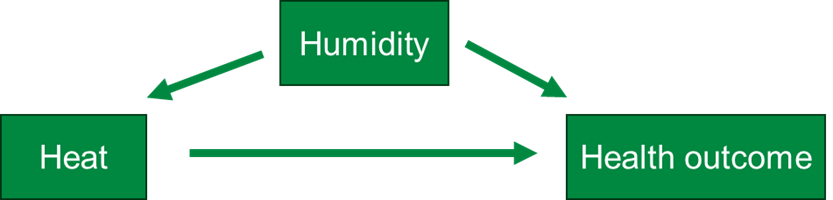
\includegraphics[width=0.8\linewidth]{Confounder} \end{center}

\textbf{Figure 2:} Humidity as confounding effect.

Humidity has been used in many epidemiological studies as a confounder when the effect of heat on health outcomes was analyzed. Researchers aim to remove the confounding influence of humidity on the relationship between heat and health outcomes by adjusting for humidity. This means the indirect effect of humidity through heat will be eliminated. Not adjusting for confounder variables, the causal effect of heat may be overestimated. This adjustment leads to a different interpretation of the estimates, as shown in the following linear model:

\[
Ε[Y│t,h]= β_0+ β_1*t+ β_2*h
\]

Y represents the health outcome of interest, t is heat, and h humidity. In this model, \(β_1\) represents the conditional total effect of heat on the health outcome at any given level of humidity. \(β_2\) represents the direct effect of humidity on the outcome. That is the causal effect of humidity on the outcome when heat is held fixed and thus blocking the humidity effect on heat.

Interpretation of estimates can however get very complex and sometimes even misleading.Consequently, the causal relation between the variables needs to be considered carefully (\citet{bald}, \citet{westreich})

One significant problem of adjusting for confounding is to potentially run into multicollinearity issues.
If heat (the exposure of interest) and humidity (the confounder) are highly correlated and both variables are included in the same regression model multicollinearity is present. Consequently, the estimates capture similar information and therefore making it difficult to interpret individual variable effects. Additionally, the precision of the estimated coefficients may be reduced. Including further variables such as calendar variables to adjust for long-term or seasonal trends can exacerbate multicollinearity if the correlation between heat and humidity varies significantly over time. Furthermore, including other variables which are highly correlated with heat and humidity will lead to further multicollinearity issues.

Baldwin et al.~suggest using alternative approaches to significance testing that do not rely solely on p-values. Furthermore, it is crucial to carefully consider the relationship between heat and humidity and their individual effects on health outcomes to avoid misleading results. (\citet{bald})

\subsection{Effect Modification and Interaction}\label{effect-modification-and-interaction}

Including humidity as an effect modifier or interaction with heat is another method to test an effect of humidity in the framework of negative health outcomes and was used in some epidemiological studies (\citet{bald}). Unlike confounding, which distorts relationships and should therefore be eliminated, effect modification and interaction are desirable biases. They provide valuable insights into how variables interact and influence outcomes, revealing inherent aspects of causal relationships that need clarification.

Often, the two terms \emph{Effect Modification} and \emph{Interaction} are used interchangeably. However, from a causal view these two concepts differ in a counterfactual perspective and slightly differ in their definition. The counterfactual perspective involves hypothetical scenarios, asking ``What if?'' questions such as, ``What if heat remained the same but humidity was lower? Would the health outcome change?''. (\citet{bours}) Counterfactual outcomes are typically written with a superscript such as \(Y^t\) and answers the question: ``What would the outcome Y be if the exposure was t?''. Or as another example \(Y^{th}\) answers the question: ``What would the outcome Y be if both exposures t and h occurred together?''. As in real-world data typically not all combinations of exposures are observed in each individual we are talking about hypothetical scenarios.\\
Both concepts are scale dependent and their presence depends on the scale used. Here, we use the risk difference scale for formal definitions.

\emph{Interaction} refers to the combined causal effect of two exposures, such as heat and humidity. \emph{Effect modification} pertains to how the causal effect of one exposure changes across different levels of a second exposure. For example, ``How does the effect of heat change across different levels of humidity?''.
Let T refer to heat, H to humidity and Y represent the outcome of interest such as heat-related death. \(Y^t\) is the counterfactual outcome under exposure t and \(Y^{th}\) is the counterfactual outcome under t and h.

Humidity (H) is \textbf{effect modifier} on the risk difference scale for the effect of heat (T) on the outcome (Y) if H is not affected by T and there are two levels of T (\(t_0\),\(t_1\)) and two levels of H (\(h_0\),\(h_1\)), such that:

\[
Ε[Y^{t_1}│H=h_1] - E[Y^{t_0}│H=h_1] ≠ E[Y^{t_1}|H=h_0]- E[Y^{t_0}|H=h_0]
\]

Effect modification indicates that the effect of heat on the outcome differs across different levels of humidity. By recognizing effect modification, public health interventions can better address how heat exposure interacts with humidity. This enables more targeted strategies to mitigate and adapt health risks associated with specific combinations of heat and humidity.

There is an \textbf{interaction} on the risk difference scale between heat (T) and humidity (H) on the outcome (Y) if there are two levels of T (\(t_0\),\(t_1\)) and two levels of H (\(h_0\),\(h_1\)), such that:
\[
Ε[Y^{t_1, h_1}] - E[Y^{t_0, h_1}] ≠ E[Y^{t_1, h_0}]- E[Y^{t_0, h_0}]
\]

Interaction requires that the joint effect of heat and humidity is different from the sum of their individual effects. If interaction is present, studying each exposure separately may not fully capture the complexity of their joint influence on the outcome. (\citet{vanderweele})

According to Baldwin and colleagues, analytical approaches to estimate interaction of effect modification are similar. They suggest that by including interaction terms or effect modifiers the main question of interest needs to be considered same as the scale of interest and the potential policy implications. (\citet{bald})

Unfortunately, the interpretation of interaction terms and effect modifiers often leads to misinterpretation and often the scale (multiplicative or additive) also is not considered correctly. Therefore, it is crucial to understand the concepts of interaction and effect modification and how to interpret them correctly.

\subsection{Data Limitations}\label{data-limitations}

The availability and quality of weather data vary across different locations all over the world. Low-income countries, like for example most african regions, often have limited access to weather data compared to high-income countries due to limited resources for data collection. Figure 3 illustrates global sub-daily weather data from the HadISD data source. This highlights the inconsistency in data coverage. Many regions in Africa, South America, and Australia have few measurements compared to Europe or the US. Such a lack of data, especially in areas prone to extreme heat events leaves gaps in our understanding and estimation of weather-related impacts on health outcomes.

Tropical and subtropical climates are characterized by high levels of humidity and heat. Unfortunately, these climates are particularly affected by these data limitations. Missing data in tropical and subtropical regions hinder our ability to comprehend the combined effects of heat and humidity on health outcomes. Therefore, epidemiological studies often do not include locations where humidity plays a significant role due to these data gaps.

Another challenge is the temporal resolution of weather data. Many studies rely on daily mean measurements, which may overlook fluctuations in heat and humidity throughout the day. It is known that heat and humidity fluctuate throughout the day. Using daily mean measurements may underestimate the effects of heat and humidity. Furthermore, correlations between heat and humidity can vary depending on the time of day, potentially impacting the findings of epidemiological studies.

Furthermore, typically weather stations are situated outside urban areas, often at airports. This may not capture urban heat effects. Additionally, as most measurements are taken outdoors, indoor and outdoor variations in heat and humidity are not accounted for.

Another limitation is that typically only relative humidity (RH) is measured at weather stations. This may not provide the most accurate representation of humidity. Deriving mass-based variables like specific or absolute humidity from RH may introduce uncertainties and bias in the estimates as menioned earlier.

In summary, the lack of weather data can result in an underestimation of the impact of humidity on health outcomes. Researchers should consider these data limitations, especially when generalizing results to different countries and weather conditions. (\citet{bald})

\begin{center}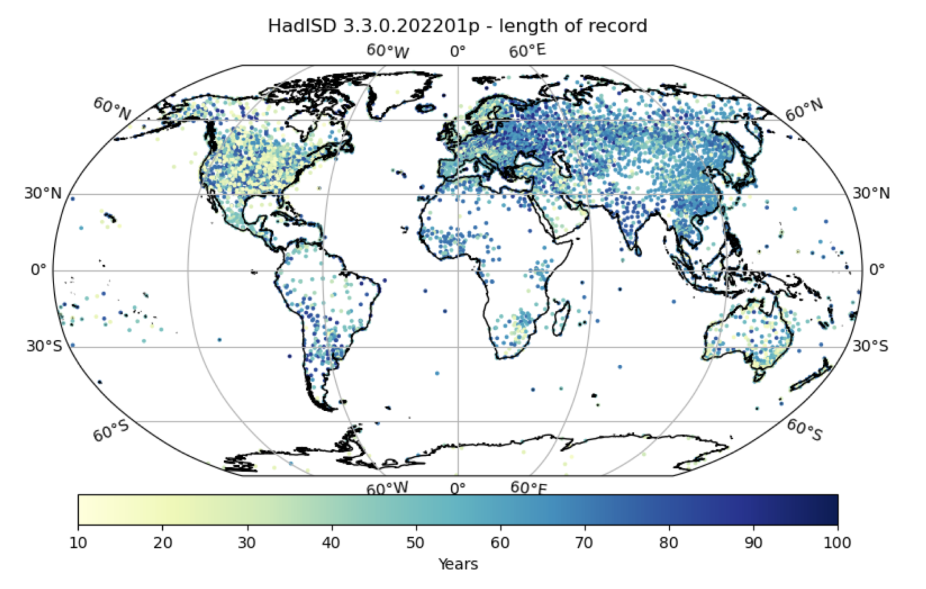
\includegraphics[width=0.8\linewidth]{hadisdimage1} \end{center}

\textbf{Figure 3:} Station coverage and length of record in HadISD (\citet{raymond})

\section{Examples}\label{examples}

Armstrong et al.~conducted a study to assess the impact of heat and humidity on daily mortality during summer months. They used a time series regression model with a distributed lag nonlinear model (DNLM) for heat, using data from 445 cities across 24 countries. Numerous different models were fitted, including different humidity levels and terms and further one model with an interaction term between heat and humidity was modeled. Model comparison using the Akaike information criterion (AIC) revealed that the best fit was achieved when humidity was included as a linear term, i.e., as confounder. One very surprisingly result was that a 23\% increase in relative humidity at the 99th percentile was associated with a 1.1\% decrease in mortality. This was a non-significant finding contrary to the expectation that humidity leads to an increase in mortality. Sensitivity analyses involving specific humidity and dewpoint yielded similar results. Considering humidity as a potential effect modifier, by including an interaction term, was not favored based on AIC criteria (\citet{armstrong}).

Baldwin et al.~criticize solely rely on AIC to determine whether an interaction term should be included in the model. Consequently, as no interaction term was used in the final model, the influence remains uncertain and raises questions about the value of its exclusion. The final model used by Armstrong et al.~included relative humidity as a linear term, thereby treating humidity as a confounder. As highlighted earlier, employing humidity as a confounder can introduce several challenges.

Armstrong et al.recognized some limitations of their study. They discussed the data gaps from tropical and less developed countries, the exclusive consideration of mortality as an endpoint, and the possibility of missing the association between humidity and mortality under specific conditions (\citet{armstrong}).

In another epidemiological study from Schwartz et al.~the effect of heat and humidity on hospital admissions for heart disease and myocardial infarction among individuals over 64 years from 12 US cities was investigated. They fitted a Poisson model for each city, incorporating regression splines to control for season and barometric pressure, and adjusting for the day of the week. Despite their broad approach, they found no evidence of an effect of humidity on hospital admissions. Possible explanations for this results are the use of relative humidity and the resulting bias. Further, considering humidity as a confounder may also explain that no effect of humidity was found. Additionally, focusing solely on individuals older than 64, who are more vulnerable to heat and sweating impairments, may have biased the study's findings. (\citet{schwartz})

Barreca conducted a study that found an effect of heat and humidity on mortality rates in the US. He used data from the Global Summary of the Day (GSOD) files, which provide detailed weather station data. The study analyzed data from 1973 to 2002, calculating specific humidity using a standard meteorological formula based on mean dew point and mean station pressure.

To estimate the effects of heat and humidity, Barreca employed an ordinary-least-squares model with the following equation:

\[
MORT_{cmy} = \sum_b \beta^b*TEMP^b_{cmy} + \sum_{b'} \alpha^{b'} * HUMID^{b'}_{cmy} + X_{cmy} \gamma + \mu_{my} + \\
\phi_{cm} + \delta_{cm} * TIME + \pi_{cm}*TIME^2 + \epsilon_{kym}
\]

In this model:

\begin{itemize}
\tightlist
\item
  MORT represents the monthly mortality rate (per 100,000 inhabitants) in county c, year y and calendar month m.
\item
  TEMP is a set of temperature variables indicating the fraction of days county c experiences mean temperatures within specific 10 °F bins (e.g., 50--60 °F).
\item
  HUMID is a set of humidity variables indicating the fraction of days county c experiences mean humidity levels within specific two-grams-of-water-vapor bins (e.g., 2--4 g/kg).
\item
  X is a vector of controls for precipitation and temperature-humidity interaction terms.
\item
  \(\mu\) represents unrestricted time effects.
\item
  \(\phi\) represents unrestricted county by calendar month fixed effects.
\item
  \(\delta_{cm}*TIME\) and \(\pi_{cm} * TIME^2\) represent unrestricted county by calendar month quadratic time trends.
  Barreca clustered the standard errors by the state of residence to account for the possibility that
  \(\epsilon\) is correlated within states, both across counties and over time. Additionally, the equation was weighted by the county population in 2000.
  He fitted different models: one model included only temperature, and another included only humidity. Both the temperature-mortality and humidity-mortality relationships followed a similar pattern. In a subsequent model, he included both TEMP and HUMID covariates. An interesting finding from this model was that both cold temperatures and low humidity levels remained significant determinants of mortality.
  Finally, he fitted a model with an interaction term between heat and humidity. The estimates from this model suggest that increasing humidity levels are more dangerous at high temperatures.
  Therefore, controlling for humidity is according to Barreca particularily important in the context of predicting distributional effects of climate change. (\citet{barr})
\end{itemize}

In a separate review, Budd examined the history and limitations of the wet-bulb globe temperature (WBGT) index, widely used since its development for the United States Army and Marine Corps in 1950. The index incorporates air temperature, mean radiant temperature, absolute humidity, and air movement as basic elements of the thermal environment. Budd identifies several limitations of the index, including its underestimation of stress in environments with restricted evaporation, challenges in interpreting its results, and limitations in the accuracy of sweat measurement due to calibration methods and instrumentation. (\citet{budd})

\section{Discussion}\label{discussion-1}

The discrepancies observed in epidemiological studies regarding the impact of humidity on health outcomes may stem from various factors. It is important to understand how to appropriately use humidity in study designs and recognize the different humidity definitions. Prioritizing mass water-vapor based variables such as specific or absolute humidity over relative humidity is a crucial step.
As discussed earlier, humidity can be considered as a confounder, effect modifier, in an interaction term with heat or component of a composite index. Each of these considerations of humidity comes with its own set of limitations.

It is essential to provide a clear research question or hypothesis when evaluating the role of humidity in studies. Researchers must be mindful of these considerations to ensure the robustness and validity of their study results.

Efforts to improve data collection are required, especially to include regions with tropical climates and low-income countries that are often underrepresented in studies. Additionally, relying solely on vulnerable populations may introduce bias, underscoring the importance of striving for a representative sample.

Humidity represents an intriguing factor worth studying further, along with heat, especially in studies investigating health effects. Planning and executing appropriate studies to examine the effects of heat and humidity requires a nuanced understanding of humidity. It is appropriate incorporation into models, and knowledge aware of potential limitations and errors.

\chapter{Risk Projections}\label{he4}

\emph{Author: Author}

\emph{Supervisor: Helmut Kuechenhoff}

\emph{Degree: Bachelor}

In many studies, the effects of climate change in the future is discussed.
In a tutorial paper (\citet{vicedo}) , statistical methods for modelling future risks due to climate devlopement are presented. In a two other papers paper the future effects of ozone and heat related are presented (\citet{domingo},\citet{chen}).

\chapter{Climate Crisis and Mental Health}\label{menh3}

\emph{Author: Nina Straub}

\emph{Supervisor: Helmut Küchenhoff}

\emph{Degree: Master}

\section{1. Introduction}\label{introduction-5}

It is widely recognized that climate change (CC) is impacting both economy and society. However, it is also increasingly acknowledged as critical factor influencing various aspects of human health. In 2009, the World Health Organisation (WHO) declared CC as one of the largest threads to human health of the twenty-first century and recognised the need for a research agenda to understand complex linkages between climate change and health \citep{worldhealthorganizationProtectingHealthClimate2009}. In following years, initiatives such as the Lancet Countdown, a global monitoring system designed to track research and support policy decisions on Health and CC, drew resources and attention to this pressing problem \citep{wattsLancetCountdownHealth2018}. Despite these efforts, some health conditions are still little researched and the impact of climate change on them is poorly understood. Among them are mental health (MH) and human well-being \citep{romanello2023ReportLancet2023a}.
According to the OECD, 20-30\% of the working population are affected by a MH condition. Mental disorders are the worldwide leading cause of years lived with disability \citep[\citet{hewlette.MakingMentalHealth2014}]{whitefordGlobalBurdenDisease2013} and a considerable burden not only for individuals but also society and economy. In 2010, the direct and indirect costs were estimated to amount to 2493 billion US dollars worldwide \citep{hewlette.MakingMentalHealth2014} and the lost economic value amounts to 4-8\% of GDP in different regions \citep{ariasQuantifyingGlobalBurden2022}. However, health care systems spend a disproportional amount on treatment. In England, MH conditions make out about 26\% of the burden of disease, but only 13\% of health expenditure are attributed to treatment \citep{hewlette.MakingMentalHealth2014}. Globally, 80\% of people do not get sufficient treatment at all \citep{worldhealthorganizationComprehensiveMentalHealth2021}.
Given the proportion of MH in global burden of disease, it seems surprising that little research has investigated how CC might affect MH. The aim of this chapter is to outline the challenges in researching the impact of CC on MH and to present research approaches on this topic. Emphasis will be placed on the methodological and statistical difficulties.

\section{2. Challenges of Quantifying Climate Change Impact on Mental Health}\label{challenges-of-quantifying-climate-change-impact-on-mental-health}

Important to notice is that CC does not directly impact MH, but rather the consequences of a changing climate, like the increase in magnitude, frequency and intensity of extreme climate events mediate the effect of CC on MH \citep{hayesClimateChangeMental2018}. The Intergovernmental Panel On Climate Change (IPCC) report identified multiple pathways how CC could impact MH. The direct pathway includes exposure to traumatic events such as floods, hurricanes or other severe weather-related events. The indirect pathway consists of the consequences of prolonged events such as drought or sea level rise that lead to displacement, food shortages or economic hardship. The last pathway, vicarious exposure or overarching/diffuse exposure refers to the long-term emotional distress caused by the awareness of the negative consequences of CC and the associated feelings of helplessness and despair \citep{intergovernmentalpanelonclimatechangeClimateChange20222023}.
Although in the IPCC report most of the adverse effects of CC on MH are assessed with ``very high confidence'', no concrete projections are given as to how many additional people will suffer from mental disorders. This is peculiar because for other health effects that are assessed with very high confidence, figures for additionally affected individuals are given \citep{intergovernmentalpanelonclimatechangeClimateChange20222023}.
The discrepancy between confidence and tangible figures is caused by multiple challenges of attributing CC to MH, which can be clustered in external and internal difficulties. The external difficulties of quantification mainly consist of the globally insufficient resources devoted to monitoring and treating MH. Although the Lancet Countdown emphasised the need to integrate MH in future CC health considerations, only five out of 16 countries included MH in their health adaption plans \citep{watts2018ReportLancet2018}. In the most recent Countdown report it was noted that the development of an indicator to cover the relations between CC and MH is still ongoing \citep{romanello2023ReportLancet2023a}. One major problems hereby is that current prevalence estimates for mental illnesses are unreliable, as mental illness is severely underdiagnosed, especially in third world countries \citep{worldhealthorganizationComprehensiveMentalHealth2021}. With the lack of a baseline, good projection estimates are difficult.
The internal difficulties of quantification evolve around the complex nature of MH itself. Hayes et al.~(2018) identified four key aspects which complicate the estimation of CC impact: Firstly, the risk of pathologizing normal stress responses due to a changing climate while adverse mental health outcomes are underdiagnosed. Secondly, multiple causal pathways in which one CC correlate can influence different MH outcomes. Thirdly, effects of CC may only become apparent after a considerable time period, which complicates the investigation of causal effects. Lastly, existing complex interactions between MH and other social determinants of health, and their relationship with CC, is insufficiently understood.

\begin{center}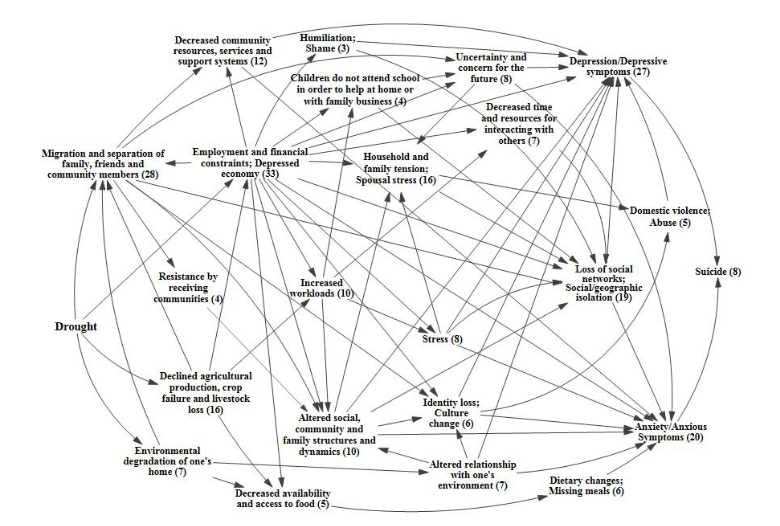
\includegraphics[width=0.8\linewidth]{work/12-mentalhealth/figures/drought_impact} \end{center}

\emph{Figure 1.} Causal process diagram of the impact of drought on the mental health outcomes depression, anxiety and suicide. Numbers in brackets are number of papers meeting the search criteria for each factor. Figure adapted from Vins et al.~(2015).

The four aspects can be illustrated by a causal process diagram, shown in Figure 1, which depicts the multiple pathways by which droughts can influence MH outcomes \citep{vinsMentalHealthOutcomes2015}. Most apparent is the economic route: Droughts have a negative impact on crop yield, influencing employment and financial stability in the agricultural sector. Financial hardship has been shown to have a negative impact on MH, leading to depression and, in severe cases, even suicide \citep[\citet{edwardsImpactDroughtMental2015}]{carletonCropdamagingTemperaturesIncrease2017}. Another causal route is the one concerned with the decreased availability of food, leading to dietary changes or famine. This can directly influence neurodevelopment of children or anxiety in adults, but also indirectly cause migration, which can lead to social isolation and loss of cultural identity, again having a negative impact on MH outcomes. To estimate the impact of droughts on MH e. g. via the migration route, it would require not only to estimate the increase and severity of droughts due to CC, but also how much migration this would cause and how many of the affected individuals would consequently develop a mental illness. This is a genuine challenge for accurate climate projections, as estimation of migration movements and the development of mental illness depend on many interrelated factors \citep{mazhinMigrationHealthCrisis2020}. Some individual linkages between events (e. g. the influence of economic hardship on MH) are well-researched. Future research needs to integrate these pathways and link them to different climate scenarios to better understand the overall causal processes and make accurate projections possible \citep{vinsMentalHealthOutcomes2015}.

\section{3. Data Sources and Methods Used to Investigate Climate Change Impact}\label{data-sources-and-methods-used-to-investigate-climate-change-impact}

To enable evidence-based policies to protect health from climate change, the WHO has identified five research priorities: (i) Assessing risks with data-based studies and, in a second step, projections and modelling, (ii) identifying the most effective interventions, (iii) guiding health-promoting mitigation and adaption decisions in other sectors, (iv) improving decision-support and (v) estimating costs \citep{worldhealthorganizationProtectingHealthClimate2009}.
While this research agenda has advanced in relation to some health outcomes, research on MH and CC is almost exclusively concerned with the first step of the first priority \citep{cianconiImpactClimateChange2020}. Methods used to describe future MH risks vary, but most quantitative studies can be grouped into a few broad categories relating to the data and measurement instruments, the study design and the statistical analysis applied \citep{charlsonClimateChangeMental2021}. The two main data sources are either official statistics or (representative) surveys. Official statistics such as mortality data or hospitalisation rates are low in cost for the researcher and have the advantage of being more objective than self-assessment questionnaires or interviews. But there are some considerable downsides. Some health outcomes, e. g. suicide rates, are often underreported, especially in countries where there is high stigmatisation. Furthermore, proxy variables sometimes have to replace variables of interest. For example, when examining the impact of drought on farmer suicide rates, occupation is not captured in the mortality statistics and one is limited to analysing rural males aged 30-60 years, assuming that they are working in agriculture \citep{carletonCropdamagingTemperaturesIncrease2017}. Surveys do not have this downside, as one can collect variables of interest and potential confounders directly, leading to more fine-grained information \citep{edwardsImpactDroughtMental2015}. However, survey data is more prone to self-selection bias and dropouts, particularly in longitudinal designs \citep{kesslerTrendsMentalIllness2008}. In addition, measuring instruments can have a low validity and data collection is costly in terms of both time and monetary resources. Which data source is chosen is largely dependent on the research question and study design.
The most common study designs are cross-sectional, followed by case-studies. Little studies attempt to model outcomes \citep{charlsonClimateChangeMental2021}.
The specific statistical analysis depends on the data source and the study design. Classic linear regression (in case of a continuous outcome, e. g. general wellbeing) and logit models (in case of binary outcome, e. g. has a mental illness -- does not have a mental illness) are most often used, but also more flexible models, allowing for non-linear effects of climatic covariates such as temperature or precipitation, are possible.
For a more detailed review on studies about environmental exposure and MH outcomes, see Charlson et al.~(2021).
It can be summarized that research concerning the impact of CC on MH is less advanced than research on other health outcomes and mostly restricted to assessing risks. A methodological difficulty inherent to research questions regarding MH is firstly the measurement of MH outcomes, relying on psychometric instruments or diagnostic interviews, and secondly the large number of potential unmeasured confounders, especially when working with official statistics.
An important motivation for researching the interactions between CC and health is that, based on a good understanding of causality and reliable projections, evidence-based measures can contribute to the adaptation of health care systems and prevent the most adverse outcomes. However, in the most frequently used cross-sectional studies on CC and MH, causal interpretations must be carefully scrutinised, particularly when dealing with complex causal processes. Different designs such as longitudinal or interventional designs, a shift towards the other WHO research priorities ii)-v) and a greater focus on non-western regions and populations may contribute to a more reliable, causal understanding.

\section{4. The Impact of Hurricanes on Posttraumatic Stress Disorder (PTSD)}\label{the-impact-of-hurricanes-on-posttraumatic-stress-disorder-ptsd}

To illustrate how the above theoretical principals are operationalised in practice, an exemplary study and its results will be described in the following. The paper ``Trends in Mental Illness and Suicidality after Hurricane Katrina'' \citep{kesslerTrendsMentalIllness2008} is concerned with the impact of one of the most destructive natural catastrophes in the history of the United States \citep{graumannHurricaneKatrinaClimatological2006}. To investigate the effect on MH, 815 pre-hurricane residents of the most affected areas were interviewed 5-8 months after the event (baseline) and again one year later (follow-up). In these interviews, data on hurricane-related stressors, demographic variables (age, gender, ethnicity, household income, education, etc.) and different MH conditions (anxiety and mood disorders, PTSD, suicidality, severity of mental illness) were collected. As the first screening interview found that individuals with higher hurricane-related stress levels chose to not participate in the study, weights were applied to the baseline hurricane-related stress variable to account for this selection bias. Additionally, the authors differentiated between individuals from the New Orleans Metropolitan area (metro subsample) and individuals from other areas (non-metro subsample). Multiple logistic regression models of the form

\[
\pi_i = P(Y_i = \text{mental illness} \mid \eta_i) = h(\eta_i) = \frac{\exp(\eta_i)}{1 + \exp(\eta_i)}
\]
with linear predictors

\[
\eta_i = \beta_0 + \beta_1 x_{i1} + \beta_2 x_{i2} + \cdots + \beta_p x_{ip}
\]

were used to investigate the different outcomes of mental illnesses. In the following, only the results of the outcome of PTSD shall be outlined.
The overall prevalence of PTSD was high in both subsamples and on both measurement points (14.9\% on baseline, 20.9\% on follow-up for the total sample), compared to the US-wide prevalence of 6\% \citep{goldsteinEpidemiologyDSM5Posttraumatic2016}. A two-tailed, within-responded paired t-test showed that prevalence increased significantly over time. Significance was driven by increase of prevalence in the non-metro subsample (11.8 vs 20.0\%, \emph{p} \textless{} 0.001), while the prevalence of the metro-subsample stagnated over time (25.9 vs 24.1\%, \emph{p} = 0.37). Recovery rate in the follow-up was low as 66.4\% of baseline cases continued to have PTSD, 16.9\% classified for another diagnosis and only 16.7\% recovered. In the logistic regression model, only two of the demographic variables, participants age and family income, had a significant influence on PTSD outcome.
The authors hypothesised that the significant increase in prevalence might be explained by an increase in hurricane-related stress. However, this hypothesis was not confirmed by the data. Regarding hurricane-related stress as outcome variable, one can find that stress decreased significantly over time in the whole sample (91.7 vs 57.5\%, \emph{p} = 0.001), but in the follow-up, stress was significantly higher in the metro subsample than the non-metro subsample (78.3 vs 51.7\%, \emph{p} \textless{} 0.001). This contrasts with the increase of PTSD in the non-metro subsample. One can conclude that higher levels of residual hurricane-related stress cannot explain the increase of PTSD prevalence over time in the non-metro subsample. In turn, when taking hurricane-related stress of the follow-up into the model as a predictor variable, one can find that it is indeed significant for both subsamples. In this final model, stress exposure was a key predictor which explained substantial variation in PTSD. The results can be seen in Table 1. Remarkable are the odds-ratios of 20.3 for severe and 12.8 for serious stress compared to individuals with no hurricane-related stress, after controlling for socio-demographic variables and diagnosis of PTSD in the baseline interview. The authors argue that, if interpreted causally, the population-attributable risk proportion of PTSD due to hurricane-related stress is 31.9\%, meaning that this proportion would be expected to remit if all hurricane-related stress would be resolved. Although the causality assumption may not be fulfilled, this statement is interesting as it could be a methodological approach to estimate additional PTSD diagnoses due to natural disasters.

\begin{table}

\caption{\label{tab:tabResults}Table 1. Effects of hurricane-related stress on PTSD outcome as shown in Kessler et al. (2008).}
\centering
\begin{tabular}[t]{l|l|l}
\hline
Severity & OR & CI\\
\hline
Severe & 20.3* & (4.9–84.6)\\
\hline
Serious & 12.8* & (3.0–53.7)\\
\hline
Moderate & 4.4* & (1.2–16.1)\\
\hline
Mild & 3.5 & (1.0–12.6)\\
\hline
None & 1.0 & \\
\hline
\$\textbackslash{}chi\textasciicircum{}2\$ (\$p\$-value) & 21.0 & (< .001)\\
\hline
\end{tabular}
\end{table}

\emph{Note.} CI, confidence interval; OR, odds ratio; PTSD, posttraumatic stress disorder. Effects estimated with multiple logistic regression model controlling for sociodemographic variables, baseline value of PTSD and subsample. Reference category were participants with no hurricane-related stress. Significance level was 0.05.

The study has four mayor limitations: First, in addition to the mentioned selection bias after the first screening, the dropout rate between measurement points was 21.9\%. Although a weight was used to account for the selection bias, it is possible that other, non-collected variables might influence participation or dropout. Second, only screening scales instead of diagnostic interviews were used for diagnosis. Hurricane-related stress was measured using self-assessment questionnaires, which is both subjective and retrospective and possibly biased by current emotional functioning. Third, although interpreted causally, hurricane-related stress and PTSD might be influenced by unmeasured common causes, influencing the observed association. Lastly, there is no true pre-hurricane baseline for the sample, and preexisting mental illness was not recorded in the survey.
The results of the presented study are partially contradicting similar studies which found a decline in PTSD over time \citep{chenIncidencePosttraumaticStress2015}. The authors hypothesise that the increase in prevalence in the non-metro subsample may be caused by greater media attention and resources being allocated to the New Orleans metropolitan region, leading to a sense of neglect and slower reconstruction of infrastructure in other areas. It is also remarked that other stressors only indirectly linked to the hurricane, such as economic stress or displacement, might influence MH outcomes. This is an interesting point of discussion, as it shows that the IPCC categorization of climate change exposures impacting MH is not as simple as outlined before. Events that fall into the category of direct exposure, such as hurricanes, might have prolonged effects on mental health outcomes, e. g. via economic hardship. This in turn makes it very difficult to attribute MH outcomes to specific CC events, as effects can be observed directly after the event, but can also have a prolonged onset. The potential causal pathways of short-term and long-term stressors on PTSD are depicted in Figure 2.

\begin{center}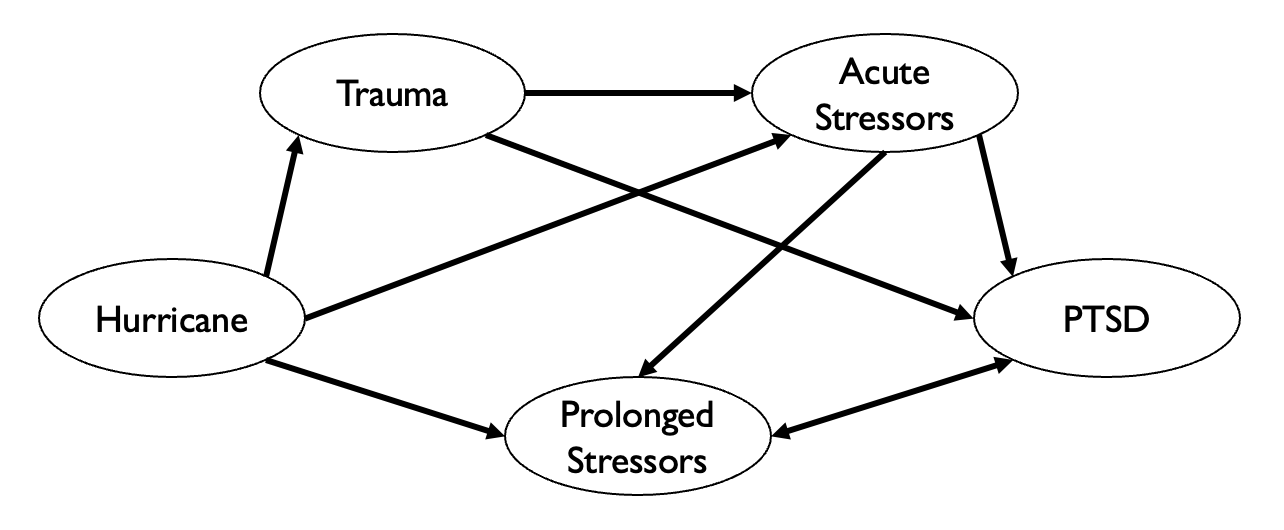
\includegraphics[width=0.75\linewidth]{work/12-mentalhealth/figures/DAG_hurricane} \end{center}

\emph{Figure 2.} Potential direct and indirect causal pathways through which hurricanes might influence the development of posttraumatic stress disorder (PTSD).

To conclude, the study shows that disaster-related stress does play a significant role in PTSD outcome. Since adverse effects are only weakly related to socio-demographic variables, efforts for sufficient treatment must extend to the entire population. High residual hurricane-related stress after two years and its strong relation to PTSD emphasizes the need for evidence-based measures to address residual stress in multiple ways, ranging from rebuilding infrastructure to providing counselling and financial support.
Although the study itself does not link the results to CC, it would be possible to draw a connection between this single, natural disaster and future CC impact on MH. According to the IPCC (2023), hurricanes are projected to increase in frequency and severity. If, as claimed in the study, hurricane-related stress plays a causal role in the development of PTSD, this increase in hurricanes would have a considerable effect on the number of individuals suffering from PTSD and would need to be taken into account for future health care adaption plans.

\section{5. Adaption and Mitigation Strategies}\label{adaption-and-mitigation-strategies}

Although the IPCC classifies the adverse impact of CC on MH to be of very high confidence, little attention has been directed to mitigation and adaption strategies for mental health and treatment systems \citep{charlsonClimateChangeMental2021}. In Berry et al.~(2018), a possible approach to deal with the high complexity of the matter is outlined. They criticise that today's policies and epidemiological research is focused mainly on individual outcomes, proximate causes and measurements on short timescales. To address the impact of CC on MH more holistically, they propose ``systems thinking'', which they define as a set of skills used to examine interacting factors that produce outcomes, predict their behaviour and design interventions. More precisely, in research they demand a mixture of CC projections and experimental designs to understand causal influences. In policy, behaviour change should be accomplished through social policy and collective actions instead of aiming at individuals. In direct actions and interventions, they demand a shift from the single-hazard perspective of e. g. extreme weather events to a strategic long-term planning accounting for an increase in those extreme events \citep{berryCaseSystemsThinking2018}.
An example for system thinking would be the protection of infrastructure to benefit MH. This sounds far-fetched, but considering that the cost of damage to critical infrastructure is estimated to increase tenfold \citep{forzieriEscalatingImpactsClimate2018}, and that these costs divert resources from public health, put pressure on the functioning of society and take up individual resources -- all factors that have a negative impact on MH -- infrastructure protection could be a promotional strategy to protect MH from the impact of CC. The causal diagram of this process is depicted in Figure 3.

\begin{center}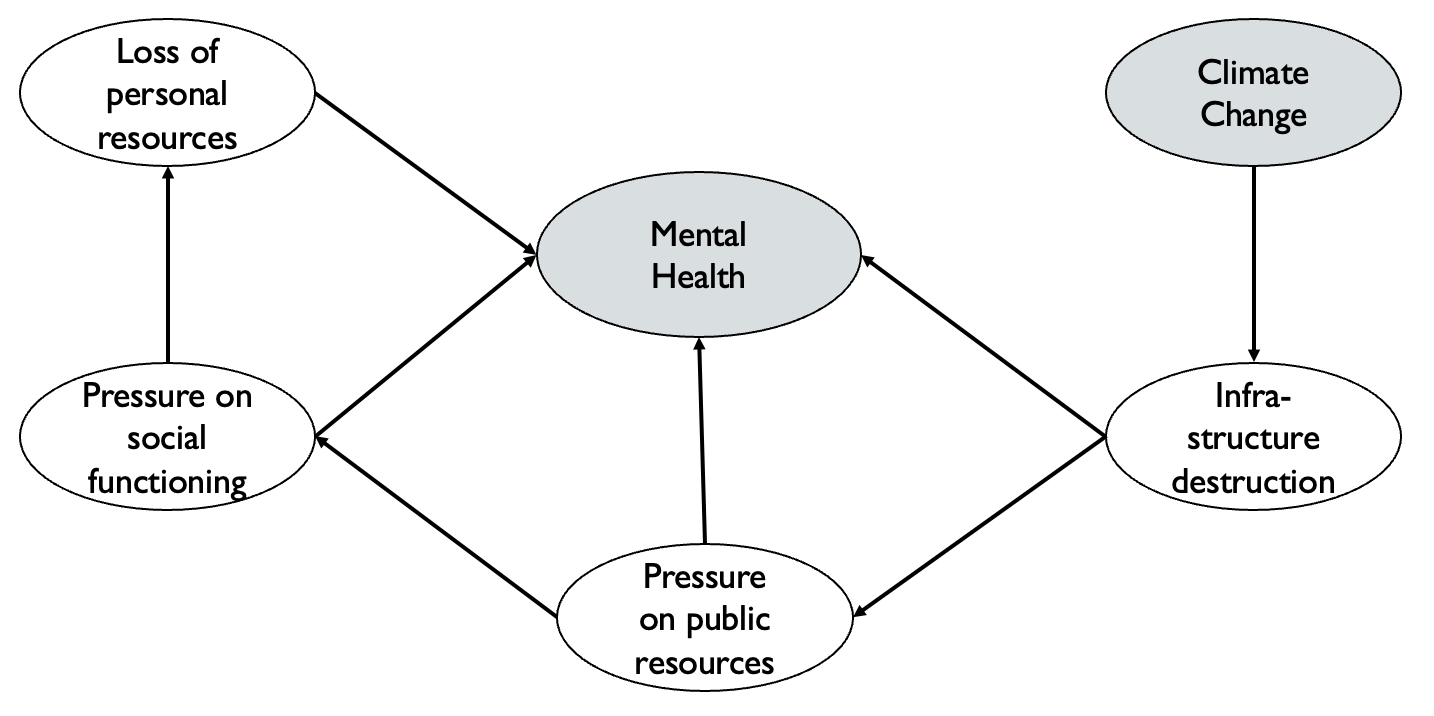
\includegraphics[width=0.75\linewidth]{work/12-mentalhealth/figures/DAG_infra_2} \end{center}

\emph{Figure 3.} Top-level process diagramm depicting linkages between climate change, infratructure and mental health, as shown in Berry et al.~(2018).

The proposal by Berry et al.~(2018) is a broad framework that may be useful to approach most of the problems discussed in this chapter. However, the individual components are yet to be tested in future research and policy designs.
On the more practical side, Hayes et al.~(2018) and Newnham et al.~(2020) proposed several practical measures that could protect MH from direct and indirect CC impact. For acute response to disaster, first-aid responders and nurses need to be trained in basic psychological first aid. It has also proven beneficial for subsequent MH outcomes to prepare people living in vulnerable areas (e.g.~near rivers that will flood more frequently in the future) for the possibility that the event might occur \citep{munroEffectEvacuationDisplacement2017}. Intermediate adaption could include capacity building for therapy and counselling, education and programmes to reduce stigma as well as community-building and preparation training for extreme weather-related events \citep{newnhamPreparingMentalHealth2020}. Long-term prevention and mitigation require governments to include MH in their strategic health planning and the development of tools to predict risks, costs and needed resources. Ultimately, a swift transition towards a carbon-neutral economy would be the most cost-effective and efficient way of protecting MH from the impacts of CC.

\section{6. Conclusion}\label{conclusion-3}

Climate change will have considerable effects on public health, including MH and wellbeing. As the latter has received little attention in research and politics, scientifically sound methods to quantify the impact of CC on MH are still being developed and research has yet not advanced from assessing the risks to estimating the costs or designing adaption strategies. Considering the importance of MH and wellbeing for individual life as well as society and economic production, more research and policy action is needed to understand this complex topic and prevent or at least attenuate the adverse impact of a changing climate on mental health.

\newpage

\chapter{References}\label{references}

\chapter{Open issue}\label{open-issue}

\emph{Author: Author}

\emph{Supervisor: Helmut Kuechenhoff}

\emph{Degree: Bachelor Master }

Further aspects of climate change

Economic, political aspects, communication

\citet{campbell} \citet{sun}

\chapter{Acknowledgements}\label{acknowledgements}

The most important contributions are from the students themselves.
The success of such projects highly depends on the students.
And this book is a success, so thanks a lot to all the authors!
The other important role is the supervisor.
Thanks to all the supervisors who participated!
Special thanks to \href{https://www.stablab.stat.uni-muenchen.de/personen/leitung/kuechenhoff1/index.html}{Helmut Küchenhoff} who enabled us to conduct the seminar in such an experimental way, supported us and gave valuable feedback for the seminar structure.
Thanks a lot as well to the entire \href{https://www.statistik.uni-muenchen.de/}{Department of Statistics} and the \href{http://www.en.uni-muenchen.de/index.html}{LMU Munich} for the infrastructure.

The authors of this work take full responsibilities for its content.

  \bibliography{book.bib,packages.bib}

\backmatter
\printindex

\end{document}
